% v2-acmsmall-sample.tex, dated March 6 2012
% This is a sample file for ACM small trim journals
%
% Compilation using 'acmsmall.cls' - version 1.3 (March 2012), Aptara Inc.
% (c) 2010 Association for Computing Machinery (ACM)
%
% Questions/Suggestions/Feedback should be addressed to => "acmtexsupport@aptaracorp.com".
% Users can also go through the FAQs available on the journal's submission webpage.
%
% Steps to compile: latex, bibtex, latex latex
%
% For tracking purposes => this is v1.3 - March 2012

\documentclass[prodmode,acmcsur]{acmsmall} % Aptara syntax

% Package to generate and customize Algorithm as per ACM style
\usepackage[ruled]{algorithm2e}
\usepackage{tikz}
\usepackage[normalem]{ulem}
\usepackage{tabularx}
\usepackage{graphicx}
\usepackage{subcaption}
\captionsetup{compatibility=false}
\usepackage{parcolumns}
\usepackage{listings,multicol,amssymb}
\renewcommand{\algorithmcfname}{ALGORITHM}
\SetAlFnt{\small}
\SetAlCapFnt{\small}
\SetAlCapNameFnt{\small}
\SetAlCapHSkip{0pt}
\IncMargin{-\parindent}
\usepackage{listings}
\newcommand{\code}[1]{\texttt{\small{#1}}}
\newcommand{\TODO}[1]{\textcolor{red}{\textbf{[TODO:#1]}}}
\newcommand{\NOTE}[1]{\textcolor{blue}{\textbf{[Note:#1]}}}
\newcommand{\LUDO}[1]{\textcolor{blue}{\textbf{[Ludo:#1]}}}
\newcommand{\KIKO}[1]{\textcolor{cyan}{\textbf{[Kiko:#1]}}}
\newcommand{\TW}[1]{\textcolor{magenta}{\textbf{[Tobias:#1]}}}
\newcommand{\JS}[1]{\textcolor{gray}{\textbf{[Justine:#1]}}}
\newcommand{\VLAD}[1]{\textcolor{orange}{\textbf{[Vlad:#1]}}}
\newcommand{\RH}[1]{\textcolor{purple}{\textbf{[Reiner:~#1]}}}
%\renewcommand{\RH}[1]{\textcolor{purple}{\textbf{[Reiner:~#1]}}}
\newcommand{\parT}{\texttt{ParT}}

%% For bold syntax highlighting in the Encore chapter
\renewcommand{\ttdefault}{lmtt}
\DeclareFontFamily{T1}{lmtt}{}
\DeclareFontShape{T1}{lmtt}{m}{n}{<-> ec-lmtl10}{}
\DeclareFontShape{T1}{lmtt}{m}{\itdefault}{<-> ec-lmtlo10}{}
\DeclareFontShape{T1}{lmtt}{\bfdefault}{n}{<-> ec-lmtk10}{}
\DeclareFontShape{T1}{lmtt}{\bfdefault}{\itdefault}{<-> ec-lmtko10}{}


% Metadata Information
%\acmVolume{9}
%\acmNumber{4}
%\acmArticle{39}
%\acmYear{2010}
%\acmMonth{3}


% Copyright
%\setcopyright{acmcopyright}
%\setcopyright{acmlicensed}
%\setcopyright{rightsretained}
%\setcopyright{usgov}
%\setcopyright{usgovmixed}
%\setcopyright{cagov}
%\setcopyright{cagovmixed}

% DOI
%\doi{0000001.0000001}

%ISSN
%\issn{1234-56789}

% Document starts
\begin{document}

% Page heads
%\markboth{G. Zhou et al.}{A Multifrequency MAC Specially Designed for WSN Applications}

% Title portion
\title{A Survey of Active Object Languages}
\author{Frank DE BOER and Vlad SERBANESCU
\affil{Centrum Wiskunde and Informatica}
Reiner H\"AHNLE
\affil{TU Darmstadt, Dept. of Computer Science}
Ludovic HENRIO and Justine ROCHAS
\affil{Universit\'e C\^ote d’Azur, CNRS, I3S}
Crystal Chang DIN and Einar Broch JOHNSEN
\affil{Department of Informatics, University of Oslo}
Marjan SIRJANI
\affil{Reykjavik University}
Ehsan KHAMESPANAH
\affil{University of Tehran}
Kiko FERNANDEZ-REYES and Albert Mingkun YANG
\affil{Uppsala University}}

% NOTE! Affiliations placed here should be for the institution where the
%       BULK of the research was done. If the author has gone to a new
%       institution, before publication, the (above) affiliation should NOT be changed.
%       The authors 'current' address may be given in the "Author's addresses:" block
%(below).
%       So for example, Mr. Abdelzaher, the bulk of the research was done at UIUC, and he
%is
%       currently affiliated with NASA.


%The abstract should be at most 100 words long and consist of short, direct sentences. It
%should state the objectives of the work, summarize the results, and give the principal
%conclusions. The title need not be repeated. Because abstracts are extracted and used
%separately, do not use the first person, do not display mathematics, and do not use
%citation reference numbers. Try to avoid starting with the words "This paper ..."
\begin{abstract} % 92 words/100
  To program parallel systems efficiently and easily, a wide range of
  programming models have been proposed, each with different choices
  concerning synchronization and communication between parallel
  entities. Among them, the actor model is based on loosely coupled
  parallel entities that communicate by means of asynchronous messages
  and mailboxes.  Some actor languages provide a strong integration
  with the object-oriented concepts; these are often called active
  object languages. This paper reviews four major actor and active
  object languages and compares them according to well-chosen
  dimensions that cover the programming paradigms and their
  implementation.
\end{abstract}
\category{D.3.2}{Programming languages}{Language Classifications}[Concurrent,
distributed, and parallel languages ]
  \category{D.3.3}{Programming languages}{Language Constructs and Features}
  [Concurrent programming structures]
% D.3.2
% The code below should be generated by the tool at
% http://dl.acm.org/ccs.cfm
% Please copy and paste the code instead of the example below.
%
%\begin{CCSXML}
%<ccs2012>
% <concept>
%  <concept_id>10010520.10010553.10010562</concept_id>
%  <concept_desc>Computer systems organization~Embedded systems</concept_desc>
%  <concept_significance>500</concept_significance>
% </concept>
% <concept>
%  <concept_id>10010520.10010575.10010755</concept_id>
%  <concept_desc>Computer systems organization~Redundancy</concept_desc>
%  <concept_significance>300</concept_significance>
% </concept>
% <concept>
%  <concept_id>10010520.10010553.10010554</concept_id>
%  <concept_desc>Computer systems organization~Robotics</concept_desc>
%  <concept_significance>100</concept_significance>
% </concept>
% <concept>
%  <concept_id>10003033.10003083.10003095</concept_id>
%  <concept_desc>Networks~Network reliability</concept_desc>
%  <concept_significance>100</concept_significance>
% </concept>
%</ccs2012>
%\end{CCSXML}

%\ccsdesc[500]{Computer systems organization~Embedded systems}
%\ccsdesc[300]{Computer systems organization~Redundancy}
%\ccsdesc{Computer systems organization~Robotics}
%\ccsdesc[100]{Networks~Network reliability}

%
% End generated code
%

% We no longer use \terms command
%\terms{Design, Algorithms, Performance}

\keywords{Programming languages, active objects, actors, concurrency, distributed systems}

%\acmformat{Gang Zhou, Yafeng Wu, Ting Yan, Tian He, Chengdu Huang, John A. Stankovic,
%and Tarek F. Abdelzaher, 2010. A multifrequency MAC specially
%designed for  wireless sensor network applications.}
% At a minimum you need to supply the author names, year and a title.
% IMPORTANT:
% Full first names whenever they are known, surname last, followed by a period.
% In the case of two authors, 'and' is placed between them.
% In the case of three or more authors, the serial comma is used, that is, all author
%names
% except the last one but including the penultimate author's name are followed by a comma,
% and then 'and' is placed before the final author's name.
% If only first and middle initials are known, then each initial
% is followed by a period and they are separated by a space.
% The remaining information (journal title, volume, article number, date, etc.) is
%'auto-generated'.

%\begin{bottomstuff}
%This work is supported by the National Science Foundation, under
%grant CNS-0435060, grant CCR-0325197 and grant EN-CS-0329609.
%
%Author's addresses: G. Zhou, Computer Science Department,
%College of William and Mary; Y. Wu  {and} J. A. Stankovic,
%Computer Science Department, University of Virginia; T. Yan,
%Eaton Innovation Center; T. He, Computer Science Department,
%University of Minnesota; C. Huang, Google; T. F. Abdelzaher,
%(Current address) NASA Ames Research Center, Moffett Field, California 94035.
%\end{bottomstuff}

\maketitle


% \NOTE{Page limit is 35 pages}


\section{Introduction}
% \TODO{Overall I think the introduction is lacking in giving a general direction to the
% article. Why are active object languages becoming important today? What will I learn from
% reading this article regarding the situation of active object languages in the current
% state of the art? How do the four languages under analysis fit within the larger
% community of active object languages or actor languages in general?
% -->> EINAR}

Designing a programming language for concurrent systems is a difficult
task. The programming abstractions provided in concurrent programming
libraries are often rather low-level and difficult to reason about,
both from the point of view of the programmer and for verification
tools. This article focuses on one family of concurrent programming
languages that tries to mitigate this problem: active object
languages.  The first and most important characteristic of this family
of languages is inherited from the actor paradigm. It relies on
organizing the program in terms of well-defined entities called
actors. Each actor is an independent entity that behaves autonomously
and that communicates with other actors through asynchronous
messages. Actors execute concurrently and communicate asynchronously,
without transfer of control. This makes the actor model attractive
\cite{Agha86-book,Erlang-book}: Using the actor model, information
sharing is simplified, programming is less error prone, analysis
becomes much easier, and programs scale better to parallel and
distributed architectures because control threads are implicit rather
than explicit in the programs.

Within actor-based languages we focus in this survey on one specific
category that uses asynchronous method calls as its communication
paradigm. Languages in this category are often called \emph{active
  object} languages. Whereas messages sent to actor are generally
selected by pattern matching over the message queue, asynchronous
method calls restrict the communication between active objects to
messages which trigger method activations. Consequently messages to an
actor can be indefinitely ignored if the actor never switches to an
appropriate state, whereas it can be statically guaranteed that
asynchronous method calls to an active object are understood.  The
basic unit of concurrency is the same in all actor languages, and the
active object languages have the same attractive features as actor
languages in general, but the way methods are called seems to pose a
rather subtle distinction. Although this merely causes minor
differences regarding the expressiveness of the different languages,
it causes considerable differences in terms of the abstractions
offered to the programmer. By supporting \emph{communication by
  asynchronous method calls}, the programming model of active object
languages is tightly integrated with the object-oriented programming
paradigm and its programming abstractions, which are familiar to most
programmers.

We start this survey by giving the historical context that led to the
existence of active object languages and that justifies their
importance. We then focus on four languages that are representative of
this language family. We start with Rebeca, which is closest to the
classical actor model \cite{Agha86-book}, but nevertheless provides
communication by a form of asynchronous method invocation. The three
other languages---ABS, ASP, and Encore---are precise representatives
of active object frameworks. Additionally, each of them implements
replies to asynchronous method calls in the form of \emph{futures}
(see Section~\ref{sec:brief-history}), which enables advanced
synchronization between the active objects.

The languages presented here come with strong support for formal
methods and verification techniques; Rebeca and ABS even make this
their main focus, having been conceived as modelling languages: actors
do not merely offer a convenient programming abstraction but also
greatly simplify static program analysis by naturally structuring
programs in entities that can serve as the basis for compositional
analyses.  ASP and Encore instead put the focus on highly optimized,
efficient implementations. Whereas these languages all fit inside the
category of active object languages, they propose different solutions
for how they support synchronization and for how much internal
concurrency they allow inside active objects. The languages are
surveyed with respect to their objectives, level of formalization, and
their implementation and tooling support. Furthermore, they are
compared with respect to a number of \emph{dimensions} in the design
space of active object languages: the degree of synchronization, the
degree of transparency, and the degree of data sharing.


This paper is organized as follows. Section~\ref{AOlanguages} presents
an overview of the actor and active object languages; it first adopts
a historical perspective, and then focuses on the four chosen
languages, presenting their design principles, the approach they
advocate, and the tools they offer.  Section~\ref{sec-implementation}
focuses on the implementation and runtime support for the presented
languages. Section~\ref{sec-discussion} discusses design aspects of
active object languages and other related languages, and
Section~\ref{sec-conclusion} concludes the paper.

\section{Active Object Languages}
\label{AOlanguages}

\subsection{A Brief History of Actor and Active Object Languages}
\label{sec:brief-history}
%\TODO{FRANK:
%	Reviewer 1 finds it too long but reviewer 2 likes it I suggest to shorten just a
%	bit\\
%	Page 3, beginning of 2.1: This is a too broad presentation starting by
%high-level languages in general and ALGOL etc. Focus the history on the relevant
%concepts.}
%
%\TODO{Also, actor languages were originally motivated within a artificial intelligence
%context. It was only later that it was identified as a general purpose concurrency model
%[Agha 90] because of the safety and liveness guarantees it provides.
%-->> FRANK: do we want to mention this???}

The development of high-level programming languages is generally
driven by the quest for suitable abstractions of the low-level
implementation details of specific underlying hardware architectures.
%The basic abstraction of
%the machine instructions for reading from and writing to memory
%locations which underlies imperative programming is the
%assignment. The low-level flow of control is further abstracted by
%means of high-level structuring mechanisms which allow the
%construction of a program in a compositional manner, e.g., sequential
%composition, choice and iterative constructs.
%One of the first major high-level imperative programming languages is
%ALGOL (short for ALGOrithmic Language) \cite{backus63cacm} which
%features procedural and functional abstractions of data and control.
%The resulting general abstraction level allows for a compositional
%construction and analysis of mainly the flow of control.
A major challenge in the development of such languages is the
high-level specification of concurrent and parallel threads of control
and their synchronization.  In process calculi like CSP \cite{Hoare85}
and CCS \cite{Milner89} independent threads of control communicate
data synchronously, e.g., via channels.  The Ada programming language
\cite{bal89acmsurv} extends this model of synchronous communication by
a rendez-vous interpretation of the execution of procedure calls and
returns.  In the shared-variable model of concurrency, threads of
control communicate and synchronize directly via shared data.  For
example, the popular object-oriented programming language Java extends
the sequential thread of control of Simula and Smalltalk, in which a
thread consists of a stack of procedure (method) calls, from one to
multiple threads in a manner resembling operating systems
\cite{goetz06java}.

The shared-variable model of concurrency underlying the Java language
requires that the developer ensures so-called \emph{thread safety};
insufficient synchronization may cause data races between threads,
rendering program behavior ``unpredictable and sometimes surprising''
\cite{goetz06java}.  To avoid data races, complex low-level
synchronization mechanisms are used, which in turn may give rise to
deadlocks and thread starvation.  The result of executing
multi-threaded programs depends on an intricate and fine-grained
granularity of interleaving. This makes their behavior difficult to
understand and to verify.  In addition, the multi-threaded concurrency
model decouples data (represented statically by classes) and control
(represented at runtime by threads), which is unintuitive and
difficult to use in a distributed setting.

The Actor model of computation \cite{Hewitt:1973,Agha86-book} departs
from the synchronous communication mechanisms described above and is
based on loosely coupled processes which interact via asynchronous
message passing.  Actors integrate and encapsulate both data and a
single thread of control, and communicate without transfer of
control. Message delivery is guaranteed but messages may arrive out of
order.  This loose coupling makes Actor languages conceptually
attractive for parallel and distributed programming; in fact, 
% e.g., in Hewitt et al. \citeyear{Hewitt:1973}
the Actor model originated from the need ``to efficiently run the
coming generation of PLANNER-like artificial intelligence languages
including those requiring a high degree of parallelism''
\cite{Hewitt:1973}.
% quote from \cite{Hewitt:1973}).
Erlang~\cite{Erlang-book} is one of the most successful actor
languages, especially because of its adoption by programmers in the
industry, and because of its massively parallel execution model
supporting a huge number of independent actors.

%\TODO{FRANK Page 4, 5th paragraph: The mentioning of Rebeca here is a bit unmotivated.
%The conceptual structure of the following paragraphs can be improved.\\
%"We start with Rebeca, which is closest to the original actor model" => What do you mean
%with original actor model? [Hewitt 73] or [Agha 86]? During the late 70s and early 80s a
%number of variations on the actor model were developed, each with wide varying semantics.
%-->> FRANK}

In the original Actor models above mentioned, the interpretation and
processing of messages are confined to and part of the overall
internal behavior of an actor. However, this does not allow a clear
separation of concerns between communication and computation, and as
such does not support a ``programming to interfaces'' discipline
\cite{Meyer92}.  A major advance in the development of high-level
programming languages is the compositional construction of programs in
terms of modules and their interfaces, which gave rise to the
object-oriented programming paradigm.  Modules are used to model
abstract data types and as such provide a powerful abstraction which
fully integrates data and control.  In the object-oriented paradigm,
modules are generalized to classes.  Classes can be characterized as
modules from which objects can be dynamically instantiated and
referred to by unique identifiers (generated at runtime).  The
concepts of classes and objects were introduced in Simula 67
\cite{dahl66cacm}, the first object-oriented language. Whereas Simula
was a sequential language with a single thread of control, it was
developed to simulate real-world (concurrent) systems and already
featured the concept of \emph{coroutines} \cite{dahl68simula}.

Active (or concurrent) object languages integrate the basic Actor
model with object-oriented concepts and as such do support interface
abstractions of implementation details.  This integration was first
proposed in ABCL~\cite{Yonezawa:1986:OCP:28697.28722}. It can be
realized by modeling a message as an asynchronous method call, thus
fixing the interpretation of a message by a corresponding method
definition.  As in the actor-based language Rebeca
\cite{DBLP:conf/csicc/SirjaniMM01,DBLP:journals/jucs/SirjaniBM05},
returning values from a method call can be modeled by another
asynchronous message.
% In Rebeca
% \cite{DBLP:conf/csicc/SirjaniMM01,DBLP:journals/jucs/SirjaniBM05}
% methods are run to completion without any further synchronization
% mechanism and do not return values.  ; in Rebeca the order of
% messages between any two actors is preserved.

The notion of method calls can be further integrated by directly
supporting return values while maintaining a loose coupling between
actors; this leads to the notion of future variables.  Futures were
originally discovered by Baker and Hewitt in the
1970s~\cite{BakerHH77}, later rediscovered by Liskov and Shrira as
promises in Argus~\cite{Liskov88}, by Halstead in
MultiLisp~\cite{Halstead:1985:MLC:4472.4478}, before finding their way
into object-oriented languages such as
Concurrent\-Smalltalk~\cite{Yokote87},
ABCL~\cite{Yonezawa:1986:OCP:28697.28722},
Eiffel$/\!/$~\cite{Caromel96}, and CJava~\cite{Cugola97}.

A future can be pictured as a mailbox that will eventually contain the
return value from a method call. Hence, the calling method may proceed
with its computation and pick up the reply later. This, however,
requires additional synchronization by means of a blocking
get-operation on the future.
%
In Creol \cite{johnsen03nik,johnsen07sosym} such a synchronization
mechanism is combined with cooperative scheduling of the method
activations of the active object, using an explicit statement to
release control.  This allows coroutine-like method call execution
inside an active object which encapsulates a single thread of
control. Cooperative scheduling permits a compositional proof theory
\cite{SDE:BoerCJ07}.

Java's multi-threaded concurrency model can be integrated with active
objects on the basis of cooperative scheduling. In the Abstract
Behavioral Specification (ABS) language \cite{JHSSS10}, Creol's
cooperative scheduling is combined with the structuring mechanism of
concurrent object groups \cite{SchaeferP10b}, originally developed for
Java.  A group of active objects has a thread pool with threads
generated by (external) asynchronous method calls and extended as a
stack of (internal) synchronous method calls.  Within a pool, at most
one thread is executing at any time and the granularity of
interleaving is explicitly controlled in the code by means of the
cooperative scheduling statements.

Caromel et al.~\citeyear{CHS:POPL04} designed ASP, an imperative,
asynchronous object calculus with transparent futures.  Their active
objects may have internal passive objects which are passed between
active objects by deep copying the entire (passive) object graph.
Unnecessary copying can be avoided with ownership type systems
\cite{clarke08aplas}.  To limit the complexity of reasoning in a
distributed and concurrent setting, ASP is restricted to ensure that
reduction is confluent and deterministic. ASP constitutes the
theoretical foundation for the ProActive language \cite{CH-book}.

Like ASP, the Encore programming language \cite{ref:encore} integrates
active objects into an object-oriented model and distinguishes among
active and passive objects (such that passive objects are owned by
active ones).  Unlike ASP, passive objects are data race-free and may
be passed by reference, due to a capability type
system~\cite{encore:kappa}.

\paragraph{Selection of representative languages}
In the remaining article we discuss these four representative active
object languages in detail. Our selection strives to cover different
aspects: modelling languages designed for analysis (ABS, Rebeca) vs.\
languages optimized for efficient execution (Encore, ProActive/ASP);
close to the classical actor model and distributed systems (Rebeca,
partially ABS, ProActive/ASP) vs.\ targeted at multi\-core platforms
(Encore); code generation (ABS) vs.\ runtime environment (Encore,
ProActive/ASP). We have also made sure that the four languages
discussed in detail have left the experimental stage and are available
in stable, public distributions. Those four language also have a
formally defined semantics allowing us to precisely compare the
behaviour of the programs written in the different languages.

% All these languages have drawn attention on different areas.
% %
% For instance, ABS is an executable modeling language with a focus on
% analysis and property-preserving code generation while, both Encore
% and ProActive, aim at efficient runtime systems for active object
% languages where Encore targets multicore platforms and ProActive has
% also been applied for the distributed setting.

\paragraph{Other high-level concurrent languages}

A discussion of other high-level concurrent languages can be found in
Section~\ref{sec:other-high-level}.

%There are several other programming languages that introduce
%high-level abstractions for concurrent programming that deviate from
%the active object approach.  JAC~\cite{ref:jac} stands for Java
%Annotations for Concurrency. It provides Java annotations that allow
%the programmer to specify the kind of parallelism that can occur
%inside a Java object from a relatively high-level perspective. It is
%possible to encode versions of actors in JAC.
%%
%The concurrency model of
%AmbientTalk~\cite{Dedecker:2006:APA:2171327.2171349} is based on the E
%Programming Language~\cite{Miller05concurrencyamong} which implements
%a communicating event-loop actor model with fully asynchronous futures
%(called promises): calls on futures trigger an asynchronous invocation
%that will be executed when the future is available and objects are
%passed by eventual reference between actors rather than by copy. This
%facilitates the creation of many small, object-level interfaces (each
%eventual reference acts as a new entry point to the actor), rather
%than a single large actor-level interface. AmbientTalk adds new
%primitives to handle disconnecting and reconnecting nodes in a network
%to support ambient-oriented programming.
%%
%In Panini \cite{LinRajan13} concurrent behavior is specified by
%composing modules (called ``capsules'') that by themselves behave
%sequentially. The granularity of concurrency is more coarse-grained
%than in active object languages and there are no explicit
%synchronization statements. Akka~\cite{haller2009scala,AkkaBook} is a
%scalable library for implementing actors on top of Java and Scala.

% \TODO{
% 	The concurrency model of AmbientTalk is based on the E Programming Language [Miller
% 	2005] which implements a communicating event-loop (CEL) actor model. Other than
% 	asynchronous futures (called promises in E) its most distinguishing feature is that
% 	objects are passed by eventual reference between actors rather then by copy. This
% 	helps support a POLA (principle of least authority) style of programming, by
% 	facilitating the creation of many small, object-level interfaces (each eventual
% 	reference acts as a new entry point to the actor), rather than a single large
% 	actor-level interface. AmbientTalk's concurrency model remains faithful to the
% 	communicating event-loop model of E but was designed as an ambient-oriented
% 	programming (AmOP) language. It adds to the CEL model a number of new primitives to
% 	handle disconnecting and reconnecting nodes in a network where connections are
% 	volatile.\\
% 	-->>[LUDO] what are we supposed to do? copy-paste?\\
% 	-->> REINER}

% \TODO{ do we add a smallnote on: Kilim, Go?}
% Reiner: rather obscure, there is not even a paper on it:
% E programming language,
%\TODO{Reiner: Panini}
%\TODO{Not sure all of them should be cited but we will decide later}

\subsection{Dimensions of Comparison between Languages}

Before we discuss details of the different active object languages, we
define the key points that we consider as important when comparing
their design.

\paragraph{Objective of the language}
Identifying the objective of the language, for which purpose it was
created, is crucial to understand the design of a programming language
and the trade-offs that have been taken between different aspects.
For example, the performance of the language can be a crucial factor
for which another aspect can be given less priority, such as the
accessibility of the language to non-experts.
% Also, a high expressiveness can be expected for a language targeting
% several platforms.  Having a precise objective for a language
% generally defines the trade-offs that have to be taken between
% several aspects.  and for this reason, in the following each
% language description will start by a brief presentation of the
% language's objectives.

\paragraph{Degree of synchronization}
There is a close relation between the design of a concurrent
programming language and the degree of synchronization that can be
expressed in it. Each language has a different set of synchronization
primitives, even though for active object languages the choices are
limited. Some languages, inspired by pure actors, have no
synchronization primitive: concurrent entities evolve in a completely
asynchronous manner and there is no instruction to wait for
some event to happen. Synchronization between processes is
due to the causal dependency created by the flow of messages.
% In this case, a forged synchronization can be obtained by choosing
% the set of messages an actor can handle at a given point in time.
Many active object languages use futures as a synchronization
mechanism.  A future represents a result that has not been computed
yet. Once the result has been computed, it can be made available automatically
or be explicitly retrieved, depending on the language design;
in each case we say that the future is \emph{resolved}.  A process can
also block waiting for a future to be resolved.
%
In active object languages, futures represent the result of
asynchronous invocations. Usually a future access is a synchronization
point. This kind of synchronization can make concurrent
programming easier, as it ensures a sequential workflow upon which the
programmer can rely.

Several active object languages support cooperative scheduling: a
thread can be suspended to handle another message\footnote{The terms
  \emph{message} and \emph{method call} are used interchangeably in
  the literature on active object languages, depending on the
  tradition that influenced language development.  Here we adopt
  the terminology that is standard for the language under
  discussion.} and resumed later.  Suspension can be triggered when
checking if a future has been resolved. This breaks the
sequential processing of a message (call), but allows programs to
be more efficient and less deadlock-prone.

Another synchronisation constraint is related to message
ordering~\cite{CMT-DisComp96}. Ensuring an order of message reception,
like point-to-point FIFO, adds some synchronisation which can lead to
a loss of efficiency and a gain in program properties. The programmer
to rely on some order of message delivery, which simplifies
programming. Often some order of message delivery is necessary for the
execution of the application, especially when the messages reach a
stateful object. Ensuring that the operations are done in the correct
order by explicit synchronisations, is more costly and more
constraining than relying on a message ordering property.


\paragraph{Degree of transparency}
This aspect concerns the number and complexity of the programming
abstractions we need to understand.  Some abstractions are
made explicitly visible in the program and some are transparent (i.e.,
hidden to the programmer). For example, if futures are transparent,
then variables pointing to futures are not explicitly distinguished
from other variables by a static type and no explicit instruction is
provided to access a future: the access is blocking if the future is
not resolved yet.

In general, the more transparency, the easier it is to write simple
programs, because the programmer does not need to know the specifics
of the concurrency model and parallelism is provided
automatically. However, for complex programs, the benefits of
transparency are weaker, because exposing the programming abstractions
can make programming, debugging, or optimization easier.

\paragraph{Degree of data sharing}
Data sharing is a crucial aspect of concurrent and distributed
programming. Depending on the target application domain and the
potential for distributed execution, the constraints regarding data
sharing can vary a lot.  The most efficient way to communicate data
between different cores on the same machine is to share the data,
whereas in a distributed setting, copying data to different consumers
is often more efficient, as it avoids communication overhead.

Efficiency aside, the complexity of the language implementation varies
with the degree of data sharing. Copying data raises the problem of
data consistency, as data modifications may not be reflected on all
copies.  Shared data access makes data consistency easier to obtain,
but creates additional communication about the shared memory,
additional synchronization, and delays. In practice, active object and
actor languages with distributed runtime systems often use a ``no
shared memory'' approach favoring data copies with very few globally
known and shared entities.

Data sharing occurs between threads and relates to the question of
which objects are active.  The first active object models were
\emph{uniform}: all objects were active with their own thread and
communicating by asynchronous method invocations only. Later,
active object models were designed with more focus on efficient access
to objects. Two additional models were proposed. First,
\emph{non-uniform} active object models, where some objects are
full-fledged active objects with their own threads, and others are
passive objects (i.e., standard objects). Second, concurrent object
groups provide a different alternative where all objects are
accessible from anywhere but the objects in the same group share the
same thread and their access is synchronized.


\paragraph{Formal semantics}
To establish formal properties of a language as well as for formal
verification, a formal semantics is required. Most active object
languages have a formal semantics, probably due to the fact that active
object and actor models were created to make concurrent entities run
more safely. A formal semantics can be used to prove generic
language properties that help programming (e.g., data
race-freedom), to prove the soundness of an implementation or of
optimisations, and to implement tools for the formal analysis of
programs. All these aspects have the potential to increase the
trustworthiness of a language and the programs written in it.
% A language with a formal semantics is overall more trustworthy; this
% is why we take this point of comparison into account.

\paragraph{Implementation and tooling support} An important dimension
of language comparison concerns the provided tool suite. Some
active object languages have been designed with certain tool support
in mind, which can explain some of the design decisions that were
taken.  The tool support around a programming language ranges from
utilities to help the programmer in designing, writing, analysing,
optimizing, and verifying their programs to utilities to support the
deployment and execution of these programs.
% Reiner : I don't understand this:
% LUDO: not sure what it meant neither - it does not add anything anyway
% This point of comparison and the previous one ensure the
% sustainability of the programming language.

\subsection{Representative Examples of Active Object Languages}

We give detailed presentations of the four languages identified at
the end of Section~\ref{sec:brief-history}. To ease comparison, each
presentation follows the dimensions introduced in the previous
section.

\subsubsection{Rebeca}

\paragraph{General presentation and objective of the language}

Rebeca (\emph{\underline{Re}active O\underline{b}j\underline{ec}ts
  L\underline{a}nguage}) is an actor-based modeling language created
in 2001
\cite{DBLP:conf/csicc/SirjaniMM01,DBLP:journals/fuin/SirjaniMSB04} as
an imperative interpretation of Agha's actor model \cite{Agha86-book}.

Rebeca is designed to model and verify concurrent and
distributed systems with the goal to bridge the gap between software
engineers and the formal methods community, by being a usable and at
the same time analyzable modeling language.  It has a formal semantics
and allows efficient compositional verification based on model
checking~\cite{DBLP:journals/jucs/SirjaniBM05,DBLP:conf/birthday/SirjaniJ11}
with state space reduction techniques
\cite{DBLP:journals/acta/JaghooriSMKM10}. Efficient analysis relies on
a number of restrictions: no shared variables, no blocking send or
receive, single-threaded actors, and non-preemptive message execution
(the execution of different messages does not interfere).

With usability as a primary design goal, Rebeca's concrete syntax is
Java-like, its computation and communication model is kept simple, and
analysis support is in the form of model checking. Rebeca is an
actor-based language without shared variables between actors and with
asynchronous message passing; there is no blocking send or receive
statement.  Therefore, learning Rebeca is easy and using model checking
tools requires far less expertise than deduction-based analyses.
%
The semantics of Rebeca helps analyzability as follows: Rebeca actors
are isolated and hence various abstractions, as well as modular and
compositional verification become more feasible.  Rebeca offers
natural modeling capabilities and efficient model checking tools for
concurrent distributed, event-based applications with pure
asynchronous message passing.  However, sometimes synchronization
among components or different communication models are vital, and the
modeling of some applications becomes cumbersome.  Following the
strategy of ``pay for what you need'',
% while core Rebeca is kept simple, 
core Rebeca can be extended in different dimensions, creating
the Rebeca family, to support modeling and analysis of a wider variety
of application domains (see Table~\ref{tab::Rebecacomparison}).

%
Extended
Rebeca~\cite{DBLP:conf/acsd/SirjaniBMS05,DBLP:journals/jucs/SirjaniBM05}
groups actors in components, with globally asynchronous communication
between components and locally synchronous communication inside a
component.
%
RebecaSys is developed to support hardware/software co-design (or
system-level design) \cite{DBLP:journals/tecs/RazaviBSKSS10} and adds
a wait statement to be faithful to the target design language,
SystemC. Global variables are added, but their use is controlled.
%
In Variable Rebeca, the modeller can use annotation to model variable
behaviours and hence define a product line of actors with different
computations \cite{DBLP:journals/jucs/SabouriK13}. Variable Rebeca
preserves the semantics of Rebeca and all members of Rebeca family can
be extended by the annotation mechanism used in Variable Rebeca.
%
Broadcasting Rebeca \cite{DBLP:conf/fsen/YousefiGK15} and Wireless
Rebeca \cite{DBLP:journals/corr/YousefiGK16} focus on modelling and
verifying of network protocols, and provide broadcasting and
multi-casting message passing, respectively.
%
Timed Rebeca
\cite{DBLP:journals/corr/abs-1108-0228,DBLP:journals/scp/ReynissonSACJIS14}
addresses real-time behaviour and is supported by customised efficient
analysis tools. Probabilistic Timed Rebeca
\cite{DBLP:journals/eceasst/JafariKSH14} extends Timed Rebeca to
capture probabilistic behavior and can only be analyzed using back-end
tools.
%
These extensions are orthogonal to other language extensions which
preserve the semantics of core Rebeca, these extensions can be added
on top of Variable Rebeca, and Broadcasting and Wireless Rebeca.

\paragraph{Language description}
We describe Rebeca using a Media Service example, shown in
Fig.~\ref{fig:rebeca-example}. Clients send requests for watching
movies to a dispatcher and the dispatcher non-deterministically
redirects requests to media servers.  The Rebeca model of Media
Service consists of a number of \emph{reactive classes}, which are
\texttt{Server}, \texttt{Dispatcher}, and \texttt{Client}, each
describing the type of a certain number of \emph{actors} (called
\emph{rebecs} in Rebeca). A reactive class specifies the size of its
message queue (Line 1) and may declare \emph{state variables} (Line
\ref{line:rebec:statevar}).  Each actor has a set of known actors to
which it can send messages. For example, an actor of type
\texttt{Dispatcher} knows three actors of type \texttt{Server} (Line
\ref{line:rebec:knownrebecs}), to which it can send
\texttt{reqForMovie} message (Lines
\ref{line:rebec:reqForMovieStart}--\ref{line:rebec:reqForMovieEnd}). Each
reactive class in Rebeca may have a constructor. Constructors have the
same name as the declaring reactive class and do not return a
value. Their task is to initialize the actor's state variables (Line
\ref{line:rebec:initState}) and to put initially needed messages in
the queue of that actor (Line \ref{line:rebec:inQueue}).

Message servers are implemented in reactive classes similar to methods
in Java.  In contrast to Java methods, message servers do not return
values and their declaration starts with the keyword \texttt{msgsrv}.
A message server is executed upon receiving its corresponding
message. Its body may include assignments, conditionals (Lines
\ref{line:rebec:switchStart}--\ref{line:rebec:switchEnd}), loops, and
message sending statements (Lines \ref{line:rebec:send:receiveMovie},
\ref{line:rebec:send:reqForMovie}). Periodic behavior is modeled by
sending messages to oneself (Line \ref{line:rebec:send:self}).  Since
communication is asynchronous, each actor has a \emph{message queue}
from which it takes the next message to serve. The ordering of
messages in these queues is FIFO. An actor takes the first message
from its queue, executes the corresponding message server
non-preemptively, and then takes the next message. The actor stays
idle if there is no message in the queue.  A \emph{non-deterministic
  assignment} statement models nondeterminism in a message server
(Line \ref{line:rebec:non-det}).  The \texttt{main} block creates
the actors of the model. In the example, seven actors are created and
receive their known actors and the parameter values of their
constructors (Lines
\ref{line:rebec:mainBegin}--\ref{line:rebec:mainEnd}).


\lstdefinelanguage{rebeca}{
  morekeywords={reactiveclass, knownrebecs, statevars, main, msgsrv, main, define, LTL, CTL, boolean, int, shortint, byte, if, else, while, for, wait, msg, reset, set, self, false, true, now, after, delay, deadline, initial},
  otherkeywords={=>,<-,<\%,<:,>:,\#,@},
  sensitive=true,
  morecomment=[l]{//},
  morecomment=[n]{/*}{*/},
  morestring=[b]",
  morestring=[b]',
  morestring=[b]"""
}

\lstset{frame=tb,
  language=rebeca,
  aboveskip=3mm,
  belowskip=3mm,
  showstringspaces=false,
  columns=flexible,
  basicstyle={\small\ttfamily},
  keywordstyle=\color{blue},
  numbers=left,
  numberstyle=\color{black},
  numbersep=5pt,
  xleftmargin=5pt,
  stepnumber=1,
  frame=none,
  breaklines=true,
  breakatwhitespace=true,
  tabsize=2,
  escapechar=|
}

\begin{figure}
\begin{lstlisting}[language=rebeca, multicols=2]
reactiveclass Dispatcher (5) {
	|\label{line:rebec:knownrebecs}|knownrebecs { Server m1, m2, m3; }
	msgsrv reqForMovie(Client client) {
		|\label{line:rebec:non-det}|byte selectedServer = ?(1, 2, 3);
		|\label{line:rebec:switchStart}|switch (selectedServer) {
			|\label{line:rebec:reqForMovieStart}|case 1: m1.reqForMovie(client);
			case 2: m2.reqForMovie(client);
			|\label{line:rebec:reqForMovieEnd}|case 3: m3.reqForMovie(client);
		|\label{line:rebec:switchEnd}|}
	}
}

reactiveclass Server (5) {
	|\label{line:rebec:statevar}|statevars {	byte maxClient; }
	Server(byte maxC)
		|\label{line:rebec:initState}|{ maxClient = maxC; }
	msgsrv reqForMovie(Client client)
		|\label{line:rebec:send:receiveMovie}|{ client.receiveMovie(); }
}
reactiveclass Client (2) {
	knownrebecs { Dispatcher disp; }
	|\label{line:rebec:inQueue}|Client() { self.watchMovie(); }
	msgsrv watchMovie()
		|\label{line:rebec:send:reqForMovie}|{ disp.reqForMovie(self); }
	msgsrv receiveMovie()
		|\label{line:rebec:send:self}|{ self.watchMovie(); }
}
main {
	|\label{line:rebec:mainBegin}|Server s1():(2),s2():(3),s3():(2);
	Dispatcher di(s1,s2,s3):();
	|\label{line:rebec:mainEnd}|Client c1(di):(),c2(di):(),c3(di):();
}
\end{lstlisting}
\caption{A simple Rebeca model}
\label{fig:rebeca-example}
\end{figure}

\paragraph{Degree of synchronization}
Following Agha's \citeyear{Agha86-book} actor model, Rebeca's actors
only communicate by asynchronous message passing, but Rebeca ensures a
FIFO point-to-point message ordering, guaranteeing some execution
order.  Extended Rebeca
\cite{DBLP:conf/acsd/SirjaniBMS05,DBLP:journals/jucs/SirjaniBM05}
adds tightly coupled component to Rebeca; actors
inside a component can be synchronized by a handshake communication
mechanism guaranteeing a causal message ordering.  RebecaSys
adds \textit{wait} statements to the syntax and a block of shared
\textit{global variables} to the model. All actors can read from and
write to global variables. Waiting on global variables introduces a
form of synchronization between actors reminiscent of cooperative
scheduling over futures, as
% and more precisely they allow one
an actor's processor is released while waiting for a given Boolean
expression to become true.

Broadcasting Rebeca adds a broadcast statement to Rebeca, but there
are no known actors, so sending a message directly to an actor is
impossible.  Wireless Rebeca adds support for multicast to neighbors
and unicast to the sender to Broadcasting Rebeca. Neighbors of an
actor are those actors that sent a message to it.  There is no
additional synchronization between two given actors in Broadcasting
and Wireless Rebeca.


\paragraph{Degree of transparency}
In Rebeca, programmers are not exposed to asynchronous communication
among actors.  The syntax is the same as for sequential programming.
There is no way to access the content of message queues, and
acknowledgments are not sent upon starting or finishing the execution
of a message server. Programmers have no control over the
interleaved execution of actors; i.e., the internal thread of an actor
takes a message from the actor's message queue and serves it in an
isolated environment, regardless of the states of other actors.  This
transparency holds for all Rebeca extensions.  Timed Rebeca and
Probabilistic Timed Rebeca change the message queue into a bag with
time-stamped messages, nevertheless, the transparency is unchanged.

\paragraph{Degree of data sharing} Rebeca is a typical \emph{uniform
  active object} language which guarantees the absence of data
sharing.  There are no shared variables among actors in
Rebeca. Parameters in messages sent among actors are passed by value.
This is even the case if a reference to an actor is passed as a
parameter; the sent reference is created as a shallow copy of the
original reference, e.g., in Fig.~\ref{fig:rebeca-example} Line
\ref{line:rebec:reqForMovieEnd} \texttt{Dispatcher} sends a request to
the server \texttt{m3} and passes the reference to the client to
\texttt{m3} as a parameter instead of passing a fresh copy of the
client actor.
%\TODO{"avoiding the creation of a new actor (e.g., Fig. 1, line 8)" => Is the correct
%line referenced? I am not sure why that line specifically illustrates why no new actor
%is
%created. I am assuming the creation of new actors is avoided because when passing a
%reference to a rebec the active object and its associated runtime are not copied. Rather
%a shallow copy of the reference is made.
%	-->>MARJAN
%}
In RebecaSys, global variables can be defined and used in a controlled
manner for wait statements as explained above.

\paragraph{Formal semantics}
To support analyzability and develop formal verification tools, Rebeca
and its extensions all have formal semantics.  The model checking
toolset of Rebeca is developed based on Rebeca's semantics
\cite{DBLP:journals/fuin/SirjaniMSB04}.
An ACP (Algebra of Communicating
Processes) semantics is defined in \cite{DBLP:conf/acsd/HojjatSMG07}.
The semantics of Timed Rebeca is defined in terms of timed automata
\cite{DBLP:journals/scp/KhamespanahSSKI15}, timed transition systems
\cite{DBLP:conf/facs2/KhamespanahSVK15}, Real-time Maude
\cite{DBLP:journals/scp/Sabahi-KavianiK15}, and floating time
transition systems \cite{DBLP:conf/facs2/KhamespanahSVK15}.  Floating
time transition systems constitute an innovative semantics for
real-time actors, resulting in a significantly  reduced
time and memory consumption when verifying timed actor models.
Formal semantics of Probabilistic Timed Rebeca is defined in terms of
Timed Markov Decision Processes in
\cite{DBLP:journals/eceasst/JafariKSH14}.

\newcolumntype{L}[1]{>{\raggedright\arraybackslash}m{#1}}
\newcolumntype{C}[1]{>{\centering\arraybackslash}p{#1}}
\newcolumntype{R}[1]{>{\raggedleft\arraybackslash}p{#1}}
\begin{table}
  \tbl{Summary of dimensions of comparison for  members of Rebeca family
    \label{tab::Rebecacomparison}}{%
    \scriptsize
    \begin{tabular}{|L{1.8cm}@{\,}|L{1.8cm}@{\,}|L{1.2cm}|L{2.4cm}@{\,}|L{1.1cm}|L{1.3cm}@{\,}|L{1.6cm}|}
      \hline
      & \textbf{Objective} & \textbf{Synchro\-nization} & \textbf{Transparency} &
      \textbf{Data Sharing} & \textbf{Formal Semantics} & \textbf{Tool Support} \\
      \hline
      \textbf{Rebeca} & Modeling and verification of distributed, concurrent
                            systems & None & (Full) message queues and  interleaving of execution  &
                                                                                                     None & SOS, ACP & Afra integrated tool, various backends \\
      \hline
      \textbf{Extended Rebeca} &  Globally asynchronous-locally synchronous
                                      systems & Locally synchro\-nous messages & As in Rebeca & None & SOS & None \\
      \hline
      \textbf{RebecaSys} & Hardware/ software co-design & Wait statement & As
                                                                                in Rebeca + synchronization over global variables & Global variables & LTS &
                                                                                                                                                             Model Checking, Simulation \\
      \hline
      \textbf{Variable Rebeca} & Product lines of actors & None & As in Rebeca
                                                                       + feature inclusion for selected product & None & SOS & Rebeca tool (after manual mapping to Rebeca)
                                                                       \\
      \hline
      \textbf{Broadcasting Rebeca} & Actors with broadcasting abilities & None
                                                      & As in Rebeca + broadcasting to all actors mechanism & None & SOS & Model
                                                                                                                           Checking \\
      \hline
      \textbf{Wireless Rebeca} & Ad-hoc mobile networks & None & As in BR
                                                                      + handling
                                                                      connectivity of
                                                                      nodes +
                                                                      multi-casting &
                                                                      None & SOS & Model
                                                                                                                                          Checking \\
      \hline
      \textbf{Timed Rebeca} & Realtime actors & Delay statement & As in Rebeca
                                                                       + Progress of time  & None & SOS,\newline RT Maude, Timed Automata, FTTS & Afra
                                                                                                                                          integrated tool, various backends \\
      \hline
      \textbf{Probabilistic Timed Rebeca} & Probabilistic real-time actors &
                                                                                  As in TRebeca & As in TR & None & SOS & Backends IMCA and Prism \\
      \hline
    \end{tabular}
  }
\end{table}

\paragraph{Implementation and tooling support}
There is a wide range of analysis and mapping tool sets for Rebeca family models:\footnote{These are
accessible from the Rebeca home page, see \url{http://rebeca-lang.org}}
\begin{itemize}
\item Eclipse-based editor with syntax highlighting for writing models and  properties
\item Compiler and build system integrated with the error location mechanism of Eclipse
\item Model checking tool for LTL and CTL model checking of Rebeca, as
  well as Floating Time Transition System generator and analyzer for
  Timed Rebeca
\item State space generators for
% compatible with 
CADP and $\mu$CRL analysis and
visualization tool sets
\item Facilities for traversing counter examples in case of property violation
\end{itemize}

% The majority 
Most of these tools and libraries are part of Afra,
the modeling and model checking IDE for Rebeca family models, but
there are aslo some
% Additionally, there are various 
stand-alone tools:
%  for the analysis of Rebeca models:
\begin{itemize}
\item Simulator backend for Rebeca and Timed Rebeca in Erlang
  \cite{DBLP:journals/scp/ReynissonSACJIS14}

\item Analysis backend for Timed Rebeca in Real-Time Maude \cite{DBLP:journals/scp/Sabahi-KavianiK15}

\item Model checking tool chain for  Probabilistic Timed Rebeca \cite{DBLP:journals/eceasst/JafariKSH14} using PRISM and IMCA

\item SysFier: model checking tool for SystemC designs  \cite{DBLP:journals/tecs/RazaviBSKSS10}

\item Sarir:  $\mu$CRL2 model checker for Rebeca \cite{DBLP:conf/acsd/HojjatSMG07}

\item Distributed model checking tool for Rebeca models \cite{DBLP:journals/eceasst/KhamespanahSMSR15}

\item Model checking tool for Broadcasting Rebeca \cite{DBLP:conf/fsen/YousefiGK15}

\item Bounded Rational LTL model checker of Rebeca  \cite{DBLP:conf/fsen/BehjatiSA09}

\item Guided search engine for deadlock detection \cite{DBLP:conf/facs2/SigurdarsonSBR12}
\end{itemize}

The dimensions of comparison for members of the Rebeca
language family are summarized in Table~\ref{tab::Rebecacomparison}.

\subsubsection{ABS}\label{sec:abs-lang}

\lstset{ morekeywords={module,export,import, from, interface, class,
    implements, await, get, new, local,release, suspend} }

\paragraph{General presentation and objective of the language}
The \emph{A}bstract \emph{B}ehavioral \emph{S}pecification language
(ABS) \cite{JHSSS10} is an object-oriented, concurrent modeling
language developed since 2009 in a series of EC-funded research
projects. %\footnote{For information about  HATS see
 % \url{www.hats-project.eu}, and for Envisage see
 % \url{www.envisage-project.eu}.}
 Its ancestors include Creol
\cite{Einar2006} and JCoBox \cite{SchaeferP10b}.

In contrast to design-oriented or architectural languages, ABS code is
fully executable. There is a simulator as well as several code
generation backends (at the moment, for Java, Haskell, and Erlang). At
the same time, ABS abstracts from features that make automatic
analysis difficult in mainstream programming languages. For example,
ABS has an object model, but it does not support code inheritance and
it enforces programming to interfaces as well as strong
encapsulation. It retains, however, modeling features that are
essential in realistic applications, for example, aliasing and
unbounded object creation.

The main design goal of ABS was to create a language that permits to
specify complex behavior of concurrent objects in a concise, natural
manner, while keeping automated analysis of that behavior feasible and
scalable.

There are extensions of ABS to model product variability
\cite{HHJLSSW12} as well as time and other resources
\cite{johnsen15jlamp} which have been used to, e.g., model and analyze
industrial applications deployed on the cloud \cite{ABHJSTW13}, but
these extensions are considered to be out of scope of the present article.

\begin{figure}
\centering
\begin{minipage}{.56\textwidth}
  \centering
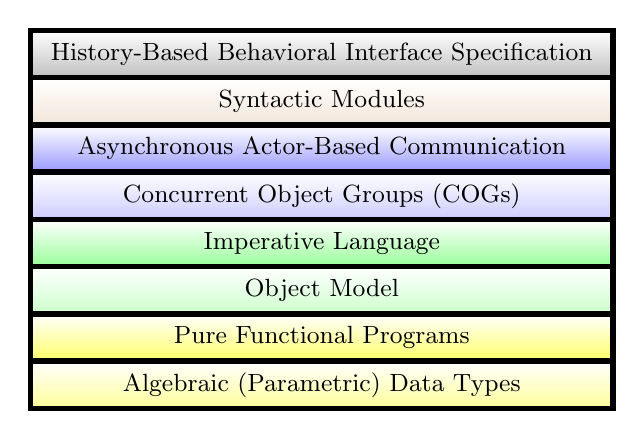
\begin{tikzpicture}[scale=1]\small
\node[rectangle,
          ,shading=axis,shading angle=180,top color=white,bottom color=black!25, line width=2pt,
          minimum width=7.4cm, minimum height=.6cm, draw] (ass) at (0,4.5)
          {History-Based Behavioral Interface Specification};

\node[rectangle,
          ,shading=axis,shading angle=180,top color=white,bottom color=brown!20, line width=2pt,
          minimum width=7.4cm, minimum height=0.6cm, draw] (mod)
          at (0,3.9) {Syntactic Modules};

\node[rectangle,
          ,shading=axis,shading angle=180,top color=white,bottom color=blue!40, line width=2pt,
          minimum width=7.4cm, minimum height=0.6cm, draw] (async)
          at (0,3.3) {Asynchronous Actor-Based Communication};

\node[rectangle,
          shading=axis,shading angle=180,top color=white,bottom color=blue!20, line width=2pt,
          minimum width=7.4cm, minimum height=0.6cm, draw] (cog)
          at (0,2.7) {Concurrent Object Groups (COGs)};

\node[rectangle,
          shading=axis,shading angle=180,top color=white,bottom color=green!40, line width=2pt,
          minimum width=7.4cm, minimum height=0.6cm, draw] (imp) at
          (0,2.1){Imperative Language};

\node[rectangle,
          shading=axis,shading angle=180,top color=white,bottom color=green!20, line width=2pt,
          minimum width=7.4cm, minimum height=0.6cm, draw] (object) at
          (0,1.5){Object Model};
\node[rectangle,
          shading=axis,shading angle=180,top color=white,bottom color=yellow!60, line width=2pt,
          minimum width=7.4cm,
          minimum height=.6cm, draw] (exp) at (0,0.9) {Pure
            Functional Programs};

\node[rectangle
          ,shading=axis,shading angle=180,top color=white,bottom color=yellow!40, line width=2pt,
          minimum width=7.4cm, minimum height=0.6cm, draw] (adt) at
          (0,0.3){Algebraic (Parametric) Data Types};
\end{tikzpicture}
\caption{Conceptual layers of the ABS language}
\label{fig:layer}
\end{minipage}\hfill
\begin{minipage}{.43\textwidth}
  \centering
  \begin{lstlisting}[numbers=left,xleftmargin=4ex,escapechar=\%]
module Services;
import Data, init, modify
  from CustomerData;

interface Service {
  Unit process(Fut<Data> fd);
}
class Server implements Service{
  Unit process(Fut<Data> fd) {
    await fd?; %\label{abs:process:awaitd}%
    Data rd = fd.get;
    rd.modify(); %\label{abs:process:sync}%
  }
}
{ // main block
Service s = new local Server(); %\label{abs:main:begin}%
Data d = new local Data();
Fut<Data> fd = d!init(); %\label{abs:main:init}%
s!process(fd); %\label{abs:main:end}%
}
\end{lstlisting}
  \caption{A simple ABS model}
  \label{fig:abs-simple}
\end{minipage}
\end{figure}


\paragraph{Language description}
The language layers of ABS are displayed in Fig.~\ref{fig:layer}.
Based on parametric (first-order) abstract data types, a simple, pure,
first-order functional language with pattern matching and strict
evaluation is defined. On top of that are objects and a standard
imperative layer. So far, this is very much like Scala-light.  The
central issue for achieving automated, scalable analysis is the design
of the concurrency model.

The concurrency model of ABS combines asynchronous
communication from the Actor model with cooperative concurrency.
We explain this concurrency model with help from the code in
Fig.~\ref{fig:abs-simple}. The unit of distribution in ABS is a
\emph{concurrent object group} (COG), which can be thought of as a set
of tasks that share a common heap and a single processor. Tasks in
different COGs can execute in parallel, but at most one task is active
in a given COG at any time.  Each task executes code owned by an
object in the COG.  New tasks are created by asynchronous method calls
to objects in the COG as well as, initially, by selecting the main
block of a module. An example of the latter is the code in
Lines~\ref{abs:main:begin}--\ref{abs:main:end}.

Line~\ref{abs:main:begin} declares and creates a new object of
interface type \lstinline{Service}, using the implementation in class
\lstinline{Server}.  The directive \lstinline{local} places the object
in the current COG. Without \lstinline{local}, a new COG would be
created together with the object. The next line declares and creates a
data object (note that interface \lstinline{Data} must be imported) in
the same COG. Hence, \lstinline{s} and \lstinline{d} share the same
heap. Line~\ref{abs:main:init} calls an initialization method
(implementation not shown) on the data. The notation ``\lstinline{!}''
denotes an asynchronous call; its effect is to create a new task in
the COG of \lstinline{d} that executes the code of \lstinline{init()}.

ABS enforces the ``programming-to-interfaces'' discipline
\cite{Meyer92} and has no other hiding mechanism than interfaces: an
object may implement several interfaces, so each pointer to the object
is typed by an interface controlling the methods available on that
pointer. Fields are not accessible via interfaces.  Asynchronous calls
do not interrupt the caller, so the statement following the call is
immediately executed. Therefore, we need a handle that we can use to
retrieve the result of an asynchronous call once its result has been
computed. In ABS, the type of such handles has a future annotation. As
can be seen in Line~\ref{abs:main:end}, it is possible to pass futures
as parameters. This makes it possible to use the result of an
asynchronous call in different places without copying it (for example,
for barrier synchronization or delegation).

After the execution of the main block has finished, two tasks in the
current COG are waiting, corresponding to the calls to
\lstinline{init()} and \lstinline{process()}, respectively. None of
them could have started while the main block was still executing,
because there was no synchronization expression in the latter. ABS
does not determine which of \lstinline{init()} and
\lstinline{process()} is started first. In fact, ABS can be
parameterized with different scheduling strategies, which can be
programmed at the functional layer \cite{bjork13isse}.  The semantics
leaves scheduling open, so the static analyzers of ABS take all
possible scheduling sequences into account.

ABS introduces \emph{cooperative concurrency} internally in COGs.
%
This means that no task is preempted (interrupted) unless
its modeler explicitly allows to do that. There are two expressions in
ABS that explicitly release control: \lstinline{release} and
\lstinline{await}. The former is unconditional while the latter has a
Boolean argument and can be used to synchronize with another task. In
particular, synchronization can depend on the resolution of futures;
i.e., cooperative scheduling can depend on the presence of return
values from asynchronous method calls.
%
In the example, a first synchronization point is reached at
Line~\ref{abs:process:awaitd} in the body of \lstinline{process()}. It
ensures that the value of the future \lstinline{fd} is available. If
\lstinline{init()} had not been scheduled before, it will be now. Once
the value of \lstinline{fd} is available, it is retrieved with a
\lstinline{get} expression. Note that \lstinline{rd} and \lstinline{d}
might well be aliased. The standard ABS idiom for asynchronous method
calls in ABS is as follows:

\begin{center}
  \lstinline{Fut<T> fx = o!m(); ... ; await fx?; T x = fx.get;}
\end{center}

In many cases of simple control flow, \lstinline{await} and
\lstinline{get} follow an asynchronous call directly. For this common
situation the abbreviation
\begin{center}
  \lstinline{T x = await o!m();}
\end{center}
is provided, which avoids the declaration of an explicit future.

Line~\ref{abs:process:sync} contains a synchronous call which is also
supported in ABS. It results in a stack-like behavior, i.e., it yields
the processor to the callee and blocks the caller until it
returns. Obviously, here we are interested only in the side effect
that \lstinline{modify()} has. Synchronous calls are only permitted inside
the COG of the caller object, in which case the caller may decide
whether to call a method synchronously or asynchronously.  Note that the entire
stack will be suspended in the case of a processor release.

The concurrency model of ABS is designed to make formal analysis
feasible.  While formal analysis of multi-threaded languages with
interleaving semantics, such as Java, is possible in principle
\cite{abraham05tcs,BlomHuisman14}, such analysis is highly complex and
seems to be out of scope at the moment for relaxed memory consistency
models.  The concurrency model of ABS carefully restricts the possible
interactions between concurrent tasks by means of cooperative
concurrency, while still allowing to describe complex, realistic
behavior of asynchronous systems.  Analysis in this setting has been
shown to be compositional \cite{AlbertAFGGMPR14,SDE:BoerCJ07} and
scalable \cite{DinTHJ15}.  Section~\ref{sec:implem-java-8} discusses a
possible implementation of cooperative scheduling for ABS.


% \TODO{Page 12: It took me some time to understand the concurrency model of ABS. It is
% explained fairly low-level. Shouldn’t one first say that COGs process concurrently and
% communicate via messages (like actors) and then talk about the concurrency within COGs
% based on preemptively scheduled tasks. Starting the explanation with references to
% interleaving semantics (page 12 top) was misleading to me.
% 	--> EINAR}

%\begin{figure}
%  \centering
%\begin{lstlisting}[numbers=left,xleftmargin=4ex,escapechar=\%]
%module Services;
%import Data, init, modify
%		from CustomerData;
%
%interface Server {
%  Unit process(Fut<Data> fd);
%}
%
%class Service implements Server {
%  Unit process(Fut<Data> fd) {
%    await fd?; %\label{abs:process:awaitd}%
%    Data rd = fd.get;
%    rd.modify(); %\label{abs:process:sync}%
%  }
%}
%{ // main block
%Server s = new local Service(); %\label{abs:main:begin}%
%Data d = new local Data();
%Fut<Data> fd = d!init(); %\label{abs:main:init}%
%s!process(fd); %\label{abs:main:end}%
%}
%\end{lstlisting}
%  \caption{A simple ABS model}
%  \label{fig:abs-simple}
%\end{figure}

%% Besser producer/consumer?

% module Services;

% interface Server {
%   Unit produce();
%   Unit consume();
% }

% class Service implements Server {
%   Int MAX = 17;
%   Int stock = 0;

%   Unit produce() {
%     while (True) {
% 	  await stock < MAX;
%       stock = stock + 1;
%       }
%   }

%   Unit consume() {
%     while (True) {
%       await stock > 0;
%       stock = stock - 1;
%       }
%   }
% }

% { // main block
%   Service s = new Server();
%   s!produce();
%   s!consume();
% }


\paragraph{Degree of synchronization}
If one attempts to retrieve a future value that is not yet ready, this
results in the blockage of its COG until the value becomes
available. Obviously, this can easily lead to deadlocks. Many
deadlocks can be avoided by guarding \lstinline{get} expressions with
an \lstinline{await} (Line~\ref{abs:process:awaitd}). Clearly, not all
deadlocks can be prevented in this manner. In practice, however,
deadlocks are easy to avoid, because synchronization points are
explicit. In addition, ABS comes with an automated deadlock analysis
tool \cite{CGM:SoSym2014} that detects potential deadlocks.  An
important point is that between explicit synchronization points
(\lstinline{release}, \lstinline{await}) no data races can occur and
computations are, therefore, deterministic.  Communication is
asynchronous in ABS, and no particular ordering has to be ensured on
request communication and service.  Obviously, execution in general is
non-deterministic unless the scheduling of service requests is also
controlled.


\paragraph{Degree of transparency}
ABS is an abstract language and implementation-specific aspects
including scheduling, message queueing, and object representation are
hidden from the modeler. Abstract data types and interfaces can be
used to postpone detailed design decisions while still permitting
analysis of those aspects of a model that are fully specified.  In ABS
the user may allow the interleaving of the tasks by explicitly
introducing task release points using \lstinline{release} and
\lstinline{await}. Using these features, the user is exposed to the
notion of asynchronous vs.\ synchronous calls, futures, and thread
interleaving, but the language still retains a compositional proof
theory \cite{SDE:BoerCJ07}.

\paragraph{Degree of data sharing} There is no designated active
object in a COG, all objects may be accessed remotely. Thus, values
from the functional language of ABS are passed by copy with a method
call whereas all objects are passed by reference (i.e., the pointer is
copied), independent of whether the called object is local or remote.
All objects in ABS have strictly private visibility, that is, they can
only access their own fields directly. The fields of any other object
must be accessed via explicit method calls.  ABS features a
\emph{concurrent object-group} model where objects in the same group
can safely be invoked directly because they are manipulated by a
single thread, invocation between different COGs is by nature
asynchronous.

\paragraph{Formal semantics}

ABS has a small step operational semantics \cite{JHSSS10,hats-d1.2}
that permits to prove soundness theorems for the various analyses that
are available for ABS. This semantics is directly expressed in terms
of rewrite rules in Maude format \cite{ClavelDELMMT07} which yields a
sound interpreter for ABS.

In addition there is an axiomatic semantics in the form of a program
logic~\cite{ref:key}. The behavior of interfaces and classes can be
specified by invariants over the histories of symbolic states as
contracts between processes.  Because preemption is excluded in ABS it
is sufficient to establish invariants upon object creation, at
explicit synchronization points and upon the termination of methods.
It is possible to prove a composition theorem for ABS about the
relation between local and global invariants \cite{Din14fac}. This
makes it possible to prove global behavioral properties of an ABS
model by (method-)local reasoning.

\paragraph{Implementation and tooling support}

As ABS has been developed with the goal of being analysable, there is
a wide range of tools available. Most of them support the full ABS
language and are fully automatic. An overview of several of the tools
is available as \cite{BFH14,WongAMPSS12}.

There is an Eclipse plug-in that provides a development environment
for ABS and integrates most tools. An alternative is the web-based ABS
collaboratory that runs in a browser and permits to try out most ABS
tools. It can be used either as a service or installed
locally. Here is a list of currently
supported tools for ABS:

\begin{itemize}
\item An editor with syntax highlighting and integrated build system,
  including compiler error location
\item An ABS simulator/interpreter with interactive debugger
\item Visualization of ABS model execution as a sequence diagram
\item Code generator backends for Erlang, Haskell,
  ProActive~\cite{rochas:hal-01065072} (see also
  Section~\ref{subsec:proactive-backend-abs}), Java
  8~\cite{serbanescuNABN14a}.
\item A glass box test case generator for \emph{concurrent} models
  \cite{AlbertAGM15}
\item A sound deadlock analysis \cite{CGM:SoSym2014}
\item A worst-case resource analysis tool that can be parameterized
  with a cost model for execution time, memory consumption,
  transmission size, peak cost and various other cost categories
  \cite{AlbertAFGGMPR14}
\item A deductive verification tool to prove  expressive, history-based
  properties \cite{ref:key,DinTHJ15} for models with an
  \emph{unbounded} number of objects and tasks
\end{itemize}


\subsubsection{ProActive and ASP}

\paragraph{General presentation and objective of the language}
ASP~\cite{CH-book} is an active object programming language
specifically designed for programming and deploying distributed
systems. ProActive is a Java library implementing the semantics of the
ASP calculus. The language is designed taking the constraints of
distributed programming into account, and relies on Remote Method
Invocation as the communication layer even though other communication
mechanisms can be used. ProActive is intended for distributed
execution; it is a middleware that supports application deployment on
distributed infrastructures such as clusters, grids and
clouds. Several choices for the design of the language can be
explained by these practical concerns.

A design choice for ASP and ProActive is to ensure maximal
transparency for the programmer: active objects and futures are
used like usual Java objects. The ProActive middleware
automatically triggers asynchronous remote invocations and
performs blocking synchronization when needed. ProActive
is thus particularly intended for Java programmers that are not
experts in concurrent and distributed programming.

A further design choice is that active objects are coarse-grained
entities. We create a dedicated thread for each of them and they come
with a quite heavy machinery for managing each object and
communicating between them. This machinery fully ensures the
distributed nature of the computation. As a consequence, using the
ProActive library, it is not possible to instantiate thousands of
active objects on the same core. Of course the number of passive
objects is not specially restricted.

Since 2010, ASP features \emph{multi-active
  objects}~\cite{HHI2013:mao} meaning that in each active object,
several threads can run in parallel and process several requests of
this active object, but each thread is still isolated inside a single
activity.  Such multi-active objects feature at the same time local
concurrency and global parallelism.

\paragraph{Language description}
In ASP, active objects coexist with
% objects that are not active; we call them
so-called \emph{passive} objects. An active object together with its
service thread(s), its passive objects, and its request queue is
called an activity.  Each passive object is placed under the
responsibility of an active object.  Only active objects are
accessible between activities. The objects that are not active are
only accessible within an activity; if those objects need to be used
by several activities, they are copied in each activity. Based on this
clear separation, the activity is the unit of distribution, which
matches the usage of one memory space per activity.  In ASP, when
using multi-active objects, several threads can execute in the same
activity, thus several threads can potentially access the objects of
an activity.

The language is transparent: method calls are automatically turned
into asynchronous requests if the targeted object is a remote active
object, otherwise it is a synchronous, local method call. Similarly,
futures are implicitly created upon asynchronous calls. Futures are
also transparently manipulated: wait-by-necessity synchronization is
automatically triggered upon an access to an unresolved future.  In
ASP, futures are first-class: they can be passed between
activities. In this case, when the future is resolved, the result is
automatically updated at all locations.

ProActive offers an API to create active objects, and a runtime for
handling ASP features. The following is an example of a ProActive
program: 
\lstset{ emph={parameters,node}, emphstyle=\itshape }
\begin{lstlisting}[numbers=none,xleftmargin=3ex]
O o = PAActiveObject.newActive(O.class, parameters, node);
T t = PAActiveObject.newActive(T.class, parameters, node);
V v = t.bar(); // implicit asynchronous method call
o.foo(v);       // v can be passed without blocking
v.foobar();     // potential wait-by-necessity on v
\end{lstlisting}
%%% THE FOLLOWING MIGHT BE TOO DETAILLED %%%
An active object is created using \code{newActive}, instead of the
\code{new} command of Java.  The \code{newActive} primitive takes as
parameters the class to instantiate, the parameters of the
constructor, and the node on which the active object will be deployed.
The variable \code{v} is the result of an asynchronous call; it is an
implicit future.
% The dynamic type of \code{v} is a future that is a dynamically created subtype of
%\code{V}.
When the future value is needed to continue execution, such as in
\code{v.foobar()}, wait-by-necessity synchronization automatically
occurs if the future is not resolved. In ProActive, proxies are used
to handle active objects and futures transparently. The transparent creation of proxies
 involves some practical restrictions: the  active
objects and futures cannot be of a primitive type or a generic type. If a future cannot
be created the call to an active object is performed synchronously.
% In ProActive, when an active object is created, it is registered in the
% RMI registry delivered with Java. A local reference to this active object is also created:
% a proxy that delegates invocations to the active object.

The principle of the multi-active object programming model is to
execute multiple requests of an active object in parallel, while
controlling the concurrency.  In practice, the programmer can declare
which requests (i.e., which methods of the active object) can be
safely executed in parallel. Such requests are called
\emph{compatible} requests. The internal scheduler of an active object
will allocate by default as many threads as necessary to run
compatible requests in parallel.  In ProActive, multi-active object
features can be used through a meta language, based on Java
annotations. The following is an example of multi-active object
annotations in ProActive:
\lstset{morekeywords={DefineGroups,Compatible,DefineRules,Group,MemberOf}
}
\begin{lstlisting}[numbers=none,xleftmargin=3ex]
@Group(name="group1", selfCompatible=true)
@Group(name="group2", selfCompatible=false)
@Compatible({"group1", "group2"})
public class MyClass {
  @MemberOf("group1")
  public ... method1(...) { ... }

  @MemberOf("group2")
  public ... method2(...) { ... }
}
\end{lstlisting}
In this example, two groups of requests are defined, each with one
method.  The two groups are declared to be compatible (and so are
their methods, by extension). The \code{selfCompatible} parameter
defines whether two different requests of the same group are allowed
to run in parallel. At runtime, a ready request is automatically
executed if it is compatible (i) with requests that are already
executing and (ii) with older requests in the queue. The first
condition prevents data races. The second condition preserves the
ordering of incompatible requests. It also prevents starvation which
would arise when requests of a group $G$ that are merely compatible
with currently executing requests are continuously overtaking requests
of another group $G'$ with which they are incompatible.

Without any annotations, a multi-active object is a mono-threaded
active object, without any local parallelism nor any possible race
condition. Programming a mono-threaded active object-based application
with ProActive is thus extremely simple. If some local parallelism is
desired, a compatibility should be declared between requests that can
be safely interleaved and for which execution order does not matter.

To define compatibility between two requests the programmer can also
use runtime information such as the request parameters or the object's
state. Programming a multi-active object-based application with
ProActive is thus somewhat more difficult than programming
mono-threaded ProActive active objects, but it is far less complex
than programming with raw threads and low-level synchronization
mechanisms while, at the same time, providing a considerable degree of
parallelism.  If even more parallelism, beyond what is possible with
request compatibility, is required, then the programmer can define
further requests as compatible and prevent undesired behavior with
traditional low-level Java synchronization primitives. Such a mixed
approach goes beyond the traditional active object model.

Further high-level specifications are available in multi-active
objects, such as request priority~\cite{henrio:hal-00916293}. To avoid
thread explosion, a limit can be set on the number of threads running
in parallel.  That can be either a hard limit restraining the overall
number of threads or a soft limit that only counts threads not
involved in wait-by-necessity synchronization.  Additionally, threads
can be limited per group.

To summarize, ASP and ProActive are based on the multi-active object
programming model.  This model is suitable for non-experts, because it
provides high-level features for distribution and safe concurrency.

\paragraph{Degree of synchronization}
In ASP, the only blocking synchronization is wait-by-necessity on a
future. As requests run until completion, potential deadlocks can
arise in case of reentrant calls, especially if no compatibility
annotation is specified.  However, synchronization only occurs when
the future value is actually needed and, in particular, future
references can safely be transmitted between activities without
requiring any additional synchronization, which limits blocking
synchronization leading to deadlocks. The ProActive middleware handles transparently the
future value transmission~\cite{HKRZ:Coregrid:2010} (a ProActive future is serializable).
Deadlocks can also be removed
by using multi-active objects especially with no limit or a soft limit
of the number of threads. Specifically, when a thread enters
wait-by-necessity, it is not counted in the soft thread limit of the
active object anymore, so the wait-by-necessity event potentially
causes the start of another request.

Communication in ASP is causally-ordered and requests are served in a FIFO order.
Overall, this restraints a bit more the communication ordering than a simple FIFO
guarantee, thus providing more properties to the programmer at the expense of an
additional delay during request emission.

\paragraph{Degree of transparency}
In ASP the programmer is not exposed at all to the notion of a future
and in a limited manner to the notion of an active object (at object
creation time only). The syntax is the same as for sequential
programming, there is no specific construct for awaiting a future
value or for performing an asynchronous call. Frequently, sequential
code can be reused unchanged in a distributed setting.  When dealing
with multi-active objects, the programmer is exposed to the notion of
parallel treatment of requests. In this case the programming model
becomes more explicit concerning concurrency aspects.

\paragraph{Degree of data sharing} ASP is a typical example of a \emph{non-uniform active
object model},
where some objects are active and the others are passive, and copied when transmitted
between activities.
ASP follows a strict policy of absence of sharing between active objects. Objects that are
not active objects are passed by copy between activities (as request parameters or request
results). Of course, this  applies also to objects that are referenced by passed
objects: a deep-copy mechanism  ensures that, when objects are transmitted
between activities, they are copied together with all their dependents on the destination
side. This mechanism, also used by RMI, slows down request invocation, because
of the time spent to transmit data, but it accelerates request treatment, because there is no
need to contact another activity to obtain the value of the request parameters. Note that
active object and future references are passed by reference.

Coherency  between different copies of a passive object is not guaranteed.  If
a user wants to ensure that an object has a unique coherent state, he should not
transmit it by copy:  transmitting it as an active object reference instead would be the best choice.

\paragraph{Formal semantics}

Several papers formalise the semantics of ASP. Caromel et
al.~\citeyear{CHS:POPL04} formalise the mono-threaded part of the
language and prove determinacy properties. In particular, they prove
that the order of future updates has no influence on the execution and
that the only source of non-determinacy in mono-threaded ASP is when
two activities can send a request to the same destination.
%
A functional fragment of the calculus has been formalized in
Isabelle/HOL~\cite{HKL:SCP11}. A specific semantics has been designed
to evaluate a functional ASP program without risk of deadlock; the
absence of deadlocks is proved in Isabelle/HOL.  The full semantics of
imperative ASP with multi-active objects is contained
in~\cite{HHI2013:mao}.


\paragraph{Implementation and tooling support}

ProActive is the Java library implementing ASP semantics.  To
transparently handle active objects and futures in ProActive, a proxy
is created for each of them. Proxies encapsulate all code required to
perform asynchronous, remote method invocations and wait-by-necessity
synchronization.

Whenever an active object or a future is given as call parameter to an
active object, it is in fact their proxy that is copied. Hence, all
copies of a proxy of an active object/future point to the same active
object/future.  A further aspect of ProActive deals with the
deployment of ASP active objects on distributed infrastructures. The
design choices of the programming language typically target a high
performance of distributed ProActive applications.  To deploy active
objects on distributed infrastructures, ProActive features a
deployment specification mechanism. Its goal is to make the physical
deployment independent from the deployment logic. This is possible by
having a binding from virtual node names, used in the source code,
pointing to machine addresses or names. In practice, this binding is
implemented in XML configuration files. Since the binding is made at
\emph{deployment time}, changing infrastructure for a given ProActive
application is localized in few files and does not require application
recompilation.  Several machines can be aggregated under a single
virtual node name in the deployment logic, for example, to provide the
virtual node with certain properties or non-functional deployment
options (such as fault tolerance or logging).


ProActive active objects, and active objects in general, provide a
convenient programming model for component-based composition of
distributed applications \cite{BHR2014:gcm}. The ProActive library
implements the GCM distributed component model. In this context, the
Vercors platform~\cite{HKM-FASE16} provides verification capacities
for ProActive components; Vercors consists of an Eclipse plugin for
designing component systems; from this point the Vercors platform can
on one hand verify the correct behavior of the application using the
CADP model-checker, and on the other hand generate an executable
ProActive/GCM code corresponding to the designed system.

\lstdefinestyle{encore}{
  language=java,
  basicstyle=\tt\color{black},
  keywordstyle=\tt\bfseries\color{blue},
  commentstyle=\it,
  aboveskip=1ex,
  belowskip=1ex,
  tabsize=2,
  columns=fullflexible,
  xleftmargin=1ex,
  resetmargins=true,
  showstringspaces=false,
  morecomment=[l]{//},
  morecomment=[s]{/*}{*/},
  escapeinside=??,
  morekeywords={assert,exclusive,stable,atomic,immutable,locked,lockfree,unsafe,trait,require,async,finish,def,consume,finish,async,J,S,var,val,shared,safe,subordinate,I,let,in,excl,then,else,wlock,wlocked,rlock,rlocked,read,thread,synchronize,linear,unpack,pack,subord,sync,bound,as,encaps,active,passive,requires,Fut,Par,Maybe,suspend,await,get}
}

\lstnewenvironment{ecode}{\lstset{style=encore}}{}
\lstnewenvironment{ecodep}[1][numbers=left]{\lstset{style=encore,#1}}{}
\newcommand{\ec}[1]{\lstinline[style=encore,basicstyle=\tt]@#1@}
\newcommand{\Upscale}{\textsc{UpScale}\xspace}

\subsubsection{Encore}\label{sec:encore}

\paragraph{General presentation}

Encore \cite{ref:encore} is a general purpose parallel language based
on active objects developed since 2014 in the EC funded \Upscale
project. %\footnote{For information about \Upscale see \url{www.upscale-project.eu}.}
 The language has been designed to excel
at scalability and rests on four pillar concepts: \textit{parallel by
  default} using the active object paradigm for coarse-grained
parallelism, \textit{independent local heaps} to promote data
locality, \textit{type-based synchronization directives} provided by a
novel capability system and \textit{coordination of parallel
  computations and low-level data parallelism} via parallel
combinators.  On top of these key ingredients, Encore stays within the
object-oriented paradigm where active objects and futures can be seen
as normal objects and, instead of interfaces, has a trait system \`a
la Scala.

\paragraph{Language description}

%\TODO{Addressed. Page 18: I had problems to understand the language description of
%Encore. It says:
%„Active objects encapsulate passive objects, and …“ and later: „In Encore, passive
%objects may be shared between active objects …“ The wording sounds contradictory to me. I
%don’t understand what encapsulation of an objects means if it is shared. Maybe the
%explanation can be improved.
%	-->> KIKO}

In Encore, active objects have their own thread of control and
communicate with each other via asynchronous messages passing.
Messages are appended to the receiver's message queue and processed
one at a time in FIFO order. Because of their internal thread of
control, active objects have an asynchronous interface, meaning method
calls return immediately with a future. In contrast, passive objects
do not have internal thread of control; hence, expose synchronous
interface. Each active object owns a local heap on which passive
objects are allocated. Ownership in this context means that the actor
is responsible for keeping track of foreign dependencies on passive
objects on its local heap, and eventually deallocate them. In Encore,
passive objects may be \emph{shared} between active objects, and
concurrent read/write access to these passive objects is supported, by
using the aforementioned capability system.

Encore is \emph{parallel by default}. On coarse-grained parallelism,
different active objects could run concurrently, while within the same
active object, the execution is sequential. Fine-grained parallel
computations can be created via the notion of tasks, for example, the
code (\ec{async \{ e \}}) contains a body \verb|e| that is
asynchronously executed and returns a future type value
immediately. Tasks are more lightweight than actors (memory-wise) and
increase the degree of asynchrony in a system.

Unlike ProActive, values resulting from method calls on active objects
and spawning of tasks have the explicit future type \ec{Fut
  t}. Futures support future chaining as well as \ec{get} and
\ec{await} operations similar to ABS. This is explained in detail
below.

\paragraph{Cooperative scheduling of active objects}

Encore supports ABS' three operators for cross-message control flow,
namely \ec{suspend} (\ec{suspend :: void -> void}), \ec{get} (\ec{get :: Fut t
-> t}), and \ec{await} (\ec{await :: Fut t -> void}).
%
Encore's \ec{await} statement only supports awaiting on the resolution
of a future, unlike ABS which supports awaiting on general Boolean
conditions (Section~\ref{sec:abs-lang}). Encore's support for future
chaining however makes \ec{await} less useful as chaining allows
triggering arbitrary operations on the resolved futures. Encore
scheduling of requests is explained in details in
Section~\ref{encore-implem}.

\paragraph{Parallelism inside active objects}

\newcommand{\bind}[0]{\ensuremath{\gg\!\!=}}
\newcommand{\prune}[0]{\ensuremath{\ll}}

Active objects provide coarse-grained parallelism via futures but do not offer
high-level language constructs for low-level coordination of parallel computations.
 To express complex coordination workflows, such as pipeline and
speculative parallelism, Encore incorporates
\parT{} collections and associated parallel combinators~\cite{ref:encore,party-coordination}.
A \parT{} collection is an abstraction that can contain asynchronous computations
and values; it is controlled via parallel combinators.
\parT{} computations have type \ec{Par t} (\ec{t} is a polymorphic type).

We explain the \parT{} combinators with the example from Fig.~\ref{fig:encore:factorisation}.
It first computes the LU and Cholesky factorisation in parallel,
spawning tasks (Lines \ref{line:encore:flu}, \ref{line:encore:chl}).
The resulting futures are lifted
%(lift :: Fut t $\to$ Par t)
(\ec{lift :: Fut t -> Par t})
%
and grouped within the same \parT{} collection
% ($\| :: Par \;t \to Par \;t \to Par \;t$),
(\ec{|| :: Par t -> Par t -> Par t}),
%
Line \ref{line:encore:par}.
Then an inversion of the matrix is performed asynchronously, using the
\ec{>>=}
%\bind{}
combinator
% ($\bind \ :: Par \ t \to (t \to Par\ t') \to Par\ t'$),
(\ec{>>=:: Par t -> (t -> Par t') ->} \ec{Par t'}),
%
Line \ref{line:encore:pipe}, which receives a function (second argument)
that is applied asynchronously to the items in the \parT{} collection, creating pipeline parallelism.
With the \ec{<<}
% \prune{}
combinator
% ($\prune \ :: (Fut \;(Maybe \;t) \to Par \;t') \to Par \;t \to Par \;t'$),
(\ec{<< :: (Fut (Maybe t) -> Par t') ->} \ec{Par t -> Par t'}),
%
Line \ref{line:encore:pipe},
the \verb|getDiagonalMtx| function is applied to the first computation that returns the inverted matrix,
stopping the remaining computations, i.e., safely stopping speculative work.

\begin{figure}[t]
\centering

\begin{lstlisting}[style=encore,numbers=left,xleftmargin=4ex,escapechar=\%,basicstyle=\small\tt,columns=fullflexible]
class Mtx
  ...
  def computeFastestDiagonal(): Par Mtx
    let mtx = this.getMtx()
        %\label{line:encore:flu}%fLU = async luFact(mtx)
        %\label{line:encore:chl}%ffChlsk = async choleskyFact(mtx)
        %\label{line:encore:par}%par = (lift fLU) || (lift fChlsk)
    in
        %\label{line:encore:pipe}%getDiagonalMtx <<  (par >>= mtvInv)
\end{lstlisting}

\caption{\label{fig:encore:factorisation}Data-pipeline and speculative parallelism in matrix factorisation.
The types of the functions are
% $\mathit{getMtx :: Mtx}$, $\mathit{luFact :: Mtx \to [Factor]}$,\\
% $\mathit{choleskyFact :: Mtx \to [Factor]}$,
% $\mathit{mtxInv :: [Factor] \to Par [Mtx]}$ and
% $\mathit{getDiagonalMtx :: Fut\!<\!\!Maybe [Mtx] \!\!> \to Par\; Mtx}$.
\ec{getMtx :: Mtx}, \ec{luFact :: Mtx -> [Factor]},
\ec{choleskyFact :: Mtx -> [Factor]},
\ec{mtxInv :: [Factor] -> Par [Mtx]} and
\ec{getDiagonalMtx :: Fut<Maybe [Mtx]> -> Par Mtx}.}
\end{figure}

The \parT{} collection and its combinators have been designed to perform
operations asynchronously, without stopping the current thread of execution.
%
\parT{} integrates well in the active object model, as it
provides a uniform interface, via parallel combinators,
to manipulate a collection of asynchronous values
and can express complex coordination workflows.
%
%This creates a collection that never blocks and executes operations on demand,
%when the values are available.
We have highlighted the most important combinators, others are
discussed in Brandauer et al.~\citeyear{ref:encore}.
%
%\parT{} integrates well in the active object model, as it
%provides a uniform interface, via parallel combinators,
%to manipulate a collection of futures and values. Complex coordination workflows
%can be easily expressed, including but not limited
%to data-pipeline and speculative parallelism.
%Furthermore, the Encore framework can
%increase the level of asynchrony of an application, spawning more lightweight tasks,
%when it detects optimisation possibilities within the \parT{} abstraction.


\paragraph{Degree of synchronization}
In Encore, the synchronization constructs \ec{get} and \ec{await}
provide the same control over futures as in ABS: the former blocks the
active object until the future is resolved and the latter releases the
current thread of execution if the future is not resolved, so that the
same active object can continue processing other messages.
Furthermore, Encore provides the \emph{future chaining} operator
($\rightsquigarrow$), which registers a callback (as an anonymous
function, aka lambda) to the future and continues processing the rest
of the message. The callback is executed when the future is resolved,
using the result of the future as the argument to the callback. This
construct allows chaining operations on futures without creating
synchronization, similar to the default behavior of futures in
AmbientTalk~\cite{Dedecker:2006:APA:2171327.2171349}, except that it
is more explicit and easier to control for the programmer. It is also
a way to mimic transparent first-class futures of ASP, except that the
callback request is only created when the future is resolved.
Communication in Encore is asynchronous but requests are served in a FIFO order.

\paragraph{Degree of transparency}

In Encore, regular and future variables are distinguished statically
(e.g., \ec{int} vs.\ \ec{Fut int}).  The \ec{get} operation explicitly
extracts the content from the future type.  Both in future management
and with parallel combinators, the programmer is exposed to the
concurrent computations being handled in Encore. However, especially
when using future chaining or parallel combinators, the scheduling and
ordering of operations is handled automatically, and the programmer
only expresses concurrency from a high-level point of view.

\paragraph{Data sharing}
Encore relies at the same time on a \emph{concurrent object group} model and on a
\emph{non-uniform active object} model where some objects are active and some others are
passive.
%\TODO{Addressed. On Line 51 you write that the "trait provides the interface-like
%feeling of OOP
%languages [..]" The usage of OOP here is not entirely appropriate: the comparison breaks
%down immediately when talking about prototype-based OOP languages like JavaScript.
%Therefore, the formulation should be adjusted to be more careful, and perhaps talk about
%"the interface-like feeling of statically-typed, Java-like OOP languages".\\
%-->  KIKO\\
%Note: Just  provide a careful formulation, I do not want a fight here even if the comment
%is perhaps not very adequate
%}

In Encore, active objects are protected by their own thread of control
while passive objects are protected by a \textit{capability} type.
Encore's type system sees passive objects as resources that are
protected by a capability that governs the permitted kind of access to
the object \cite{ref:encore}. A capability is built from a trait and a
\textit{kind}. The trait provides the interface-like feeling of
statically-typed, Java-like, OOP languages while the \textit{kind}
states the ``protection'' that the interface provides. By changing a
keyword, the \textit{kind}, the interface changes the protection
level. For instance, by changing the \textit{kind} from
\textit{exclusive} to \textit{lock-free}, the interface changes the
protection from an actor-like to a lock-free implementation. Like in
RebecaSys, this creates controlled data sharing.

The Encore capabilities form the hierarchy  in
Fig.~\ref{fig:capa-tree}. \emph{Exclusive capabilities} are local to
one thread and linear capabilities may be transferred between
concurrent computations without data races by dynamic means of
concurrency control.
%
\emph{Shared capabilities} may be shared across
concurrent computations, because they encapsulate
a means of protection against concurrent access: \emph{pessimistic
capabilities} like locks and actors serialize computation;
%
\emph{optimistic capabilities} like STM and lock-free capabilities allow
parallel operations, but use a roll-back schema when
conflicts arise.
%
\emph{Immutable} and \emph{read-only capabilities} are
always safe to access concurrently because of the absence of
writes.
%
Finally, \emph{subordinate capabilities} allow constructing aggregates
of objects whose data race-freedom stems from their proper
encapsulation inside another capability.

Encore's capabilities are created from traits, and importantly,
different traits in the same class can construct different
capabilities. This allows a substructural treatment of objects,
e.g., taking a pair and splitting it into two disjoint halves,
which can be pointed to and modified separately.
%
A more experimental feature of Encore is the combination of certain
capabilities to express, e.g., an active object with a partially
synchronous interface (like a priority channel), or active objects
which are encapsulated inside other active objects to create
constrained active object topologies.

\begin{figure}[t]
  \centering
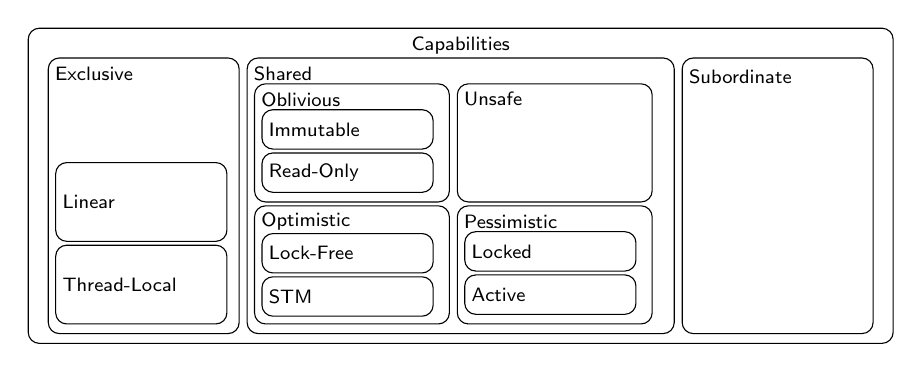
\begin{tikzpicture}[font=\sf\scriptsize,align=center,rounded corners]
  \node[draw,text width=10.75cm] {Capabilities\\%
    \mbox{\tikz{\node[draw,text width=2.25cm,minimum height=3.5cm] {Exclusive\\[1cm]
          \mbox{\tikz{\node[draw,text width=2cm,minimum height=1cm] {Linear};}}
          \mbox{\tikz{\node[draw,text width=2cm,minimum height=1cm] {Thread-Local};}}
        };}}
    \mbox{\tikz{\node[draw,text width=5.25cm,minimum height=3.5cm] {Shared\\
          \mbox{\tikz{\node[draw,text width=2.3cm,minimum height=1.5cm] {Oblivious\\
                \mbox{\tikz{\node[draw,text width=2cm,minimum height=.5cm] {Immutable};}}
                \mbox{\tikz{\node[draw,text width=2cm,minimum height=.5cm] {Read-Only};}}
              };}}
          \mbox{\tikz{\node[draw,text width=2.3cm,minimum height=1.5cm] {Unsafe\\[.85cm] \mbox{}
              };}}\\
          \mbox{\tikz{\node[draw,text width=2.3cm,minimum height=1.5cm] {Optimistic\\
                \mbox{\tikz{\node[draw,text width=2cm,minimum height=.5cm] {Lock-Free};}}
                \mbox{\tikz{\node[draw,text width=2cm,minimum height=.5cm] {STM};}}
              };}}
          \mbox{\tikz{\node[draw,text width=2.3cm,minimum height=1.5cm] {Pessimistic\\
                \mbox{\tikz{\node[draw,text width=2cm,minimum height=.5cm] {Locked};}}
                \mbox{\tikz{\node[draw,text width=2cm,minimum height=.5cm] {Active};}}
              };}}
        };}}
    \mbox{\tikz{\node[draw,text width=2.25cm,minimum height=3.5cm] {Subordinate\\[2.75cm] \mbox{}};}}
  };
\end{tikzpicture}
%  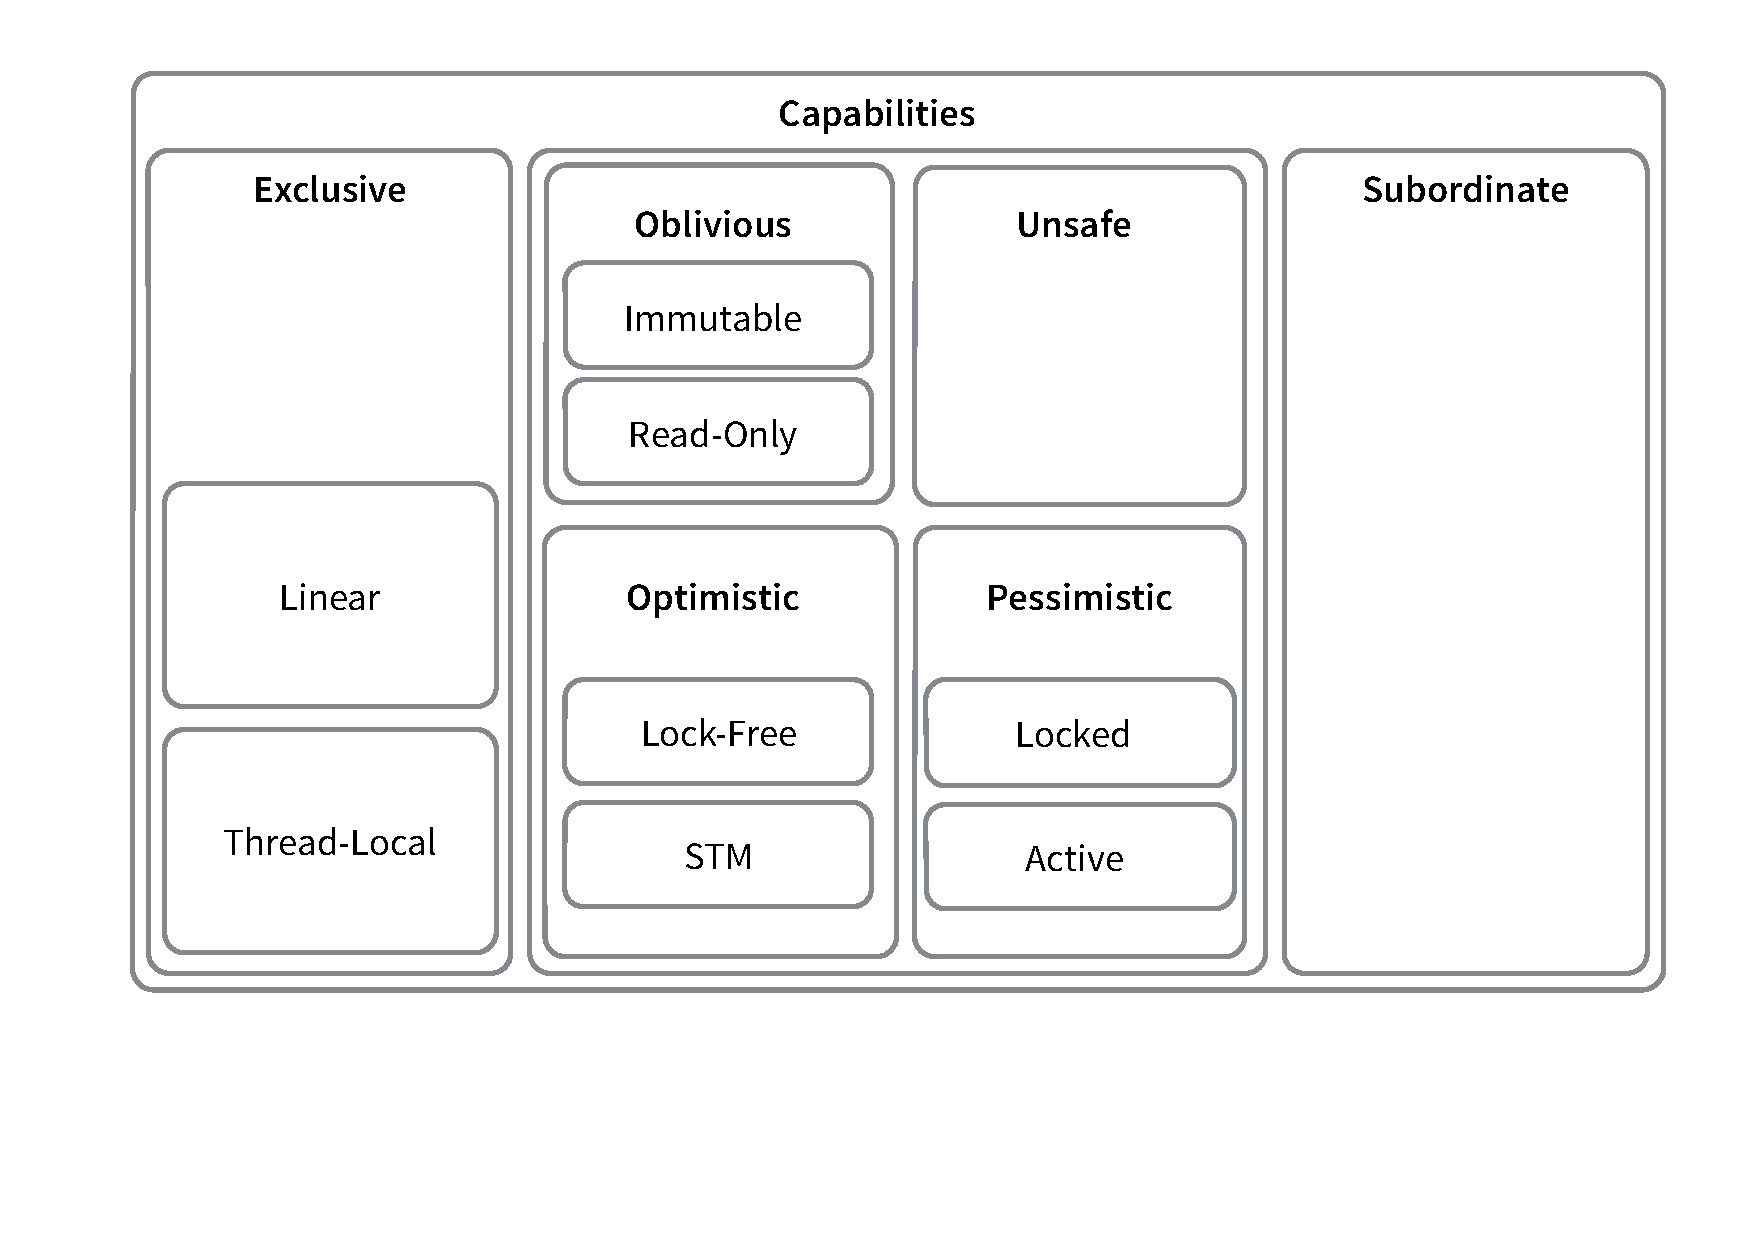
\includegraphics[scale=.25]{pictures/capabilities}
  \caption{Encore capability hierarchy}
  \label{fig:capa-tree}
\end{figure}

\paragraph{Formal semantics}
The Encore concurrency model is formalized \cite{ref:encore} using a
small step operational semantics. Parallel combinators are formalized
as well, including a soundness proof with the implicit task
parallelism model
\cite{encore:parallel-combinators-thesis,party-coordination}.  The
capability type system is formalized with proofs of soundness and data
race-freedom \cite{encore:kappa}.

\paragraph{Implementation and tooling support}
Encore is a relatively new programming language and there is limited
tooling support. However, the Encore compiler can emit readable C code
which can be analyzed and debugged using any available tool that works
with the C11 standard.  The currently supported Encore tools are:

\begin{itemize}
\item Emacs and Atom editors with syntax highlighting and compiler error support
\item Support for the GDB/LLDB interactive debugger
\item Vagrant support for rapid installation of Encore in a virtual machine
\end{itemize}

\section{Implementation of Active Objects}\label{sec-implementation}

This section describes the implementation of the active object
programming models introduced above.  Active object languages claim to
support more intuitive, easier-to-use concurrent programming models
than traditional programming languages, while retaining the latter's
efficiency (or even improve upon it). Hence, implementation aspects of
active object languages are as important as their design. Their
discussion exhibits a number of difficult, partially unsolved,
research questions. They constitute an essential part of this survey.

The implementation of a programming language can be done in a standalone manner with
a full compiler tool chain or it can be implemented as an API inside
an established language. A third way to implement an active object
language is to cross-translate it to another language with a code
generation backend, i.e., a translator that captures the semantics of
the source language. The advantage of the latter solution is that
several backends can be supported, targeting different execution
platforms, optimized for different needs.

Analogous to Section~\ref{AOlanguages}, in the following subsection we
establish the dimensions of comparison regarding the runtime system
and efficient implementation of the language semantics. In subsequent
sections we use these dimensions to compare different active object
implementations.
% , and say whether they rely on a translation to another language, or
% have their own runtime, or are implemented as a middleware layer,
Whenever meaningful, we show experiments illustrating under which
conditions an implementation outperforms existing solutions.

%
%\TODO{Do all languages have support for distribution? I would expect this to have a
%large
%impact on the implementation and definitely be a very relevant dimension along which the
%different languages can be classified.\\
%--> VLAD (also check what was there ; not sure this should be cited as a new dimension
%but it could be part of data sharing and object referencing)\\
%To the best of my knowledge : Encore and Rebeca has no support for distribution ;
%ProActive has ; ABS is a bit more complicated depending on the backend}

\subsection{Dimensions of Comparison between Implementations}

The fact that an implementation has support for distribution or not has a strong
influence on the different dimensions, for example concerning the possibility to share
data between active objects, but also concerning garbage collection. An active object
being an independent entity  from the point of view of thread existence and scheduling,
it is in several language considered as the unit of distribution. Among the languages
presented here, ASP is clearly targeting distributed implementations, and some
distributed implementations of ABS exist. Rebeca and Encore implementations do not
support distribution for the moment.


\paragraph{Thread creation and scheduling}

Active object languages implemented on top of an existing programming
language (or runtime system) must comply with the constraints given by
the underlying platform.  In the case of multi-threading, some
underlying platforms feature light threads, whereas in some frameworks
(e.g., Java) each thread is a physical one (i.e. a thread of the operating system). In
that case, one can
consider implementing light threads on top of physical threads. Having
light threads is crucial when the goal of an active object language is
to scale to a large number of active objects located on the same
machine, or to cope with cooperative multi-threading when tasks can be
interrupted.  It becomes a challenge to implement this behavior in
programming languages that do not support thread serialization, like
Java.  Concerning this dimension, the following questions are raised
in general: how are active objects and requests mapped to threads?
Should the thread be a physical thread or a virtual one?

\paragraph{Data sharing and object referencing}

This aspect addresses the question whether objects are shared between
active objects and, if so, how.  Active objects encapsulate their
state such that they are independent from each other.  In general,
active objects prevent race conditions by allowing a single entity (an
ABS COG or an active object) access to each object. This principle
partitions the memory which limits or prevents data races.
In practice, this requires to distinguish between objects that can be
remotely accessed (by asynchronous invocations), objects that have to
be copied when exchanged between active objects, and objects that can
be shared safely (e.g., immutable objects).  Accessing objects in
another activity might cause communication overhead and delay the
treatment of requests. Copying objects might lengthen the initial
request invocation, because of the serialization time, but accelerates the
request treatment. Handling copied objects also involves coherency
issues.
% Different languages take different choices on which objects are
% copied and how the copy and the referencing of objects is handled.
% Some implementation also create a pool of immutable objects that are
% easier to share without risk of data-race-condition.
To communicate, objects must have a way to reference each other.
% In particular, to send a request to an active object, one must have
% a reference to it and be able to access it.  In distributed
% settings, an efficient active object implementation cannot rely on a
% global shared memory, because it would be too costly.
The ability to reference and interact with remote objects raises even
more questions in a distributed setting where a global address space
is generally too costly.  How to efficiently and safely share
information between active objects is an open challenge and different
kinds of data sharing strategies have been proposed in active object
implementations.


\paragraph{Error handling}

% Among non-functional features an active object implementation can
% provide, we can mention how errors are handled.
The handling of errors is easier in a sequential program where the
context of an operation is known. In a concurrent setting, if a task
raises an error, this will have to be reported to another task. When
the second task is informed of the error it is difficult to react
properly as the conditions that raised the error are not fully
known. In distributed implementations exception handling is even more
complex, because an exception might reveal node or communication
failures.  Additionally, active object implementations can offer
recovery mechanisms to allow systems to recover after one or more
active objects have failed.

\paragraph{Garbage collection}

Garbage collection is important for active object applications to
scale and to be perennial. In most cases, the garbage collecting
strategy must be implemented to fit a particular active object
language. Even for active object languages built upon a host language
with garbage collection, that language can only provide partial
garbage collection. The central question for active object
implementations is when \emph{active} objects are no longer needed,
i.e., when they cease having to serve new requests.  Again, the
question is even more complex in the case of distributed
implementations, because reference counting is scattered.

\subsection{Java 8 Backend for ABS}
\label{sec:implem-java-8}

The ABS language allows several programming paradigms and design
patterns offering both a functional model as well as an
object-oriented model.  Annotations allow  defining custom schedulers
to ease the development of batch systems and workflows. The main goal
of the Java~8 backend for ABS \footnote{Available at \url{https://github.com/vlad-serbanescu/abs-api-cwi/tree/LocalOnly}} is to translate these models into
production code to be executed in a parallel or distributed
environment. The challenge is to generate real memory structures and
execution instances, while being aware of the possible resource
limitations, communication bottlenecks, latencies and performance
issues, as these issues are not easily observable at a modeling level. The version of the
Java 8 backend for ABS presented below does not support distributed execution.


\paragraph{Thread creation and scheduling}

ABS contains constructs for the two finest levels of granularity in
parallel computing, scheduling method calls within an object and
scheduling object execution within a task. Cooperative scheduling used
to be a major implementation challenge before Java~8, because a
straightforward implementation would match a Java thread to each
method call and a thread pool to each object. Hence, an asynchronous
method call caused the creation of a new thread inside a thread pool
along with the start of this thread executing the method. There is a
mismatch because a Java object is a thread pool containing the
threads originating from the methods invoked by that object. In ABS,
however, at most one method executes on an object at any time, so
creating a new thread for each fine-grained ABS method call is
wasteful. It scaled badly due to the huge number of threads that
occupy a large portion of the heap and seriously compromised the
performance of previous Java backends for ABS.

\paragraph{Cooperative scheduling of active objects using Java 8}

%\TODO{The comparison between the Java 8 backend and the old Java backend feels out of
%place. From the text I gather that the Java 8 backend seems to be a strict upgrade to
%the
%old Java backend. The performance comparison between both does not seem relevant to this
%article.\\
%	The comparison between the Java 8 and ProActive backend for ABS seems much more
%	relevant as it highlights another design trade-off.\\
%	-->> VLAD\\
%	Note: I would rather  explain why the old Java backend is representative of a
%	significant set of implementations of Active objects (you can include local ProActive
%	here)
%	\\
%%	Error handling and garbage collection are two dimensions that are not discussed for
%%	the Java 8 backend.\\
%%	-->> VLAD\\
%}

New features of Java 8 allow method calls to be wrapped into
lightweight lambda expressions such that they can be put into a
scheduling queue of an \texttt{ExecutorService} to which the running
objects are mapped, significantly reducing the number of idle threads
at runtime. The current implementation, illustrated in Fig.~\ref{abs8:coop}
shows active objects having a demand-driven approach
and only creating a physical thread once they have a method to execute inside their queue
and
the \texttt{ExecutorService} has a thread available in its pool. Finally, when all messages are
blocked or the active object's queue is empty the thread is ended and released back to the pool
of the \texttt{ExecutorService}. The impact of this approach will be evaluated in an ABS example that will compare the
performance of the Java 8 bcakend with the ProActive backend for ABS discussed in Section \ref{subsec:proactive-backend-abs}.
The only drawback is that if a method call contains a
recursive stack of synchronous calls, this stack needs to be saved
upon encountering an \texttt{await} statement, which cannot be realized with lambda
expressions. To solve this problem, such a call stack would be modeled as continuation
functions
and then be saved as lambda expressions. These lambda expressions would be ordered, such that,
once released, the continuations would execute and maintain the correct logic of the program.

%% Note (RH): this is not the place for a detailed discussion of alternatives
%
% To solve this issue we focused our research in two directions:
% \begin{itemize}
% \item On every preemption, we calculate the continuation and enqueue
%   the rest of the call into the message queue.
% \item On every preemption, we try to optimally suspend the message
%   thread until the continuation of the call is released.
% \end{itemize}
% The first direction is still in progress, as we have a fundamental
% technical limitation in the JVM/compiler. Forcing the JVM to turn the
% rest of a method into another method call in the object's message
% queue is a major challenge. The second direction however offers the
% following possible scenario that is illustrated in Figure
% \ref{abs8:coop}:

\begin{figure}
  \centering
  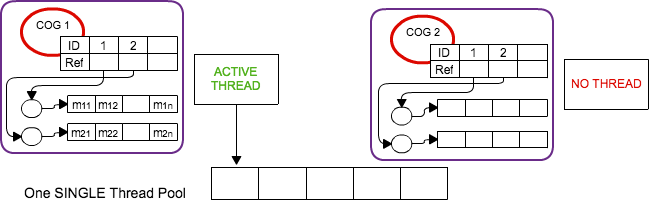
\includegraphics[scale=0.45]{./pictures/ABS8dd.png}
  \caption{Thread Creation and Scheduling}
  \label{abs8:coop}
\end{figure}



%that on every preemption we try to optimize
%the suspension of the message thread until the call is released for
%continuation. In this scenario each asynchronous call is a message
%delivered to the callee's queue and all objects in the same COG
%compete for one thread. A sweeper thread decides which task from the
%existing queues is instantiated and becomes available for execution.
%A \emph{single} global thread pool executes available tasks based on a
%work stealing mechanism.

%\RH{Please replace cog B in Fig. 8 with vertical dots to save
%  space. Replace cog with COG. Repace cog/Sweeper A with cog/sweeper
 % 1. Use different indices for each m.}

%%% Note (RH): I don't understand this, should be left out, too detailed
% The remaining problem is the situation when an execution of multiple
% synchronous calls is preempted. This results in a call stack and
% context that must be saved within a thread. To do this the executing
% thread from the pool is suspended and will compete again, upon
% release, with the other available tasks in the COG for selection by
% the Sweeper Thread to be made available to the thread pool. However
% the Sweeper Thread gives priority to live threads ready for execution
% against new messages that have not yet become threads.

\paragraph{Data sharing and object referencing}

In the Java 8 backend for ABS objects are organized into COGs, each
running on one thread. When objects are created, they are assigned to a
new or existing COG. All invocations on the object are executed on
the thread of the COG to which the object is assigned.
Data that is shared among distributed objects is passed through lambda
expressions that are sent as serialized messages between the objects,
hence all data passed in a distributed system must be
serializable. With COGs residing on the same machine, for example
applications that run on a multi-core machine, all data is passed as
arguments to lambda expressions or synchronous method calls in
Java~8. Objects can keep references to any other object in any COG as
inner fields. Similar to data sharing, objects must be serializable to
be transferred between distributed objects. Furthermore, the generated
classes will be automatically loaded on all machines that require an
object of a particular type, such that remote objects can invoke
methods on serialized references they receive.

\paragraph{Error handling}
In the Java 8 backend, all software errors are handled by Java's exception
handling mechanism. All the exception definitions that ABS provides
can directly be translated into extensions of the Exception class in Java.
Furthermore the error handling syntax that ABS provides to
pattern matching exceptions can directly be translated to Java's
try-catch mechanisms at compile time.

\paragraph{Garbage Collection}
Garbage collection in the Java 8 backend requires only bookkeeping futures
that lock messages on actors from separate COG's, such that an actor
responsible for completing a future can notify the awaiting actors to resume execution.
Once this notification is completed these references are deleted and
the process of freeing memory is handled completely by
the Java's garbage collector.


%\paragraph{Example and experiments}

%To measure the improvement provided by Java 8 features, we benchmark a
%simple example that is illustrated in Fig.~\ref{abs8:sf}. In the
%example we have one COG containing an object which receives a large
%number of messages stored in its queue. This message recursively calls
%a function that creates a large stack frame after which a message is
%sent to a different COG to run in parallel a CPU-intensive
%trigonometric function. The object is then suspended to await the
%result of this function, resulting in a large stack frame that needs
%to be saved in order to allow the next message from the queue to run
%on the COG.  We varied the number of recursive calls, the total number
%of messages in the object's queue, and the complexity of the function
%to compare performance with the previous Java backend that mapped each
%ABS method call to a separate Java thread. The results are shown in
%Fig.~\ref{abs8:ex}. The performance figures presented are for one
%object that is running 10--10000 method invocations, each with a
%varying stack frame (1--1000 recursive calls) and awaits the
%completion of a trigonometric function that reiterates a random number
%(1--1000 times) before completing. Finally we tested the backend in terms of scalability
%and performance using a Map Reduce example which will be presented in Section \ref{sec:implem-proactive},
%together with the ProActive backend for ABS.

%\begin{figure}
%\centering
%\begin{minipage}{.53\textwidth}
%  \centering
%	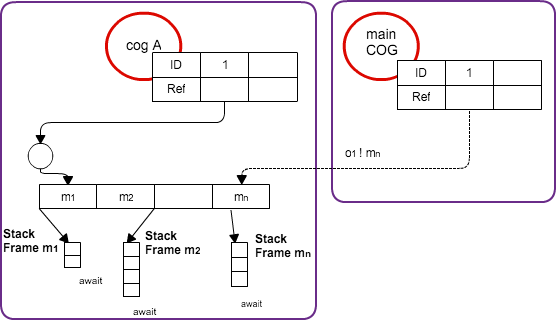
\includegraphics[scale=0.35]{pictures/scenarioj8.png}
%	\caption{Cooperative Scheduling Test Scenario}
%	\label{abs8:sf}
%\end{minipage}
%\begin{minipage}{.46\textwidth}
%  \centering
%   	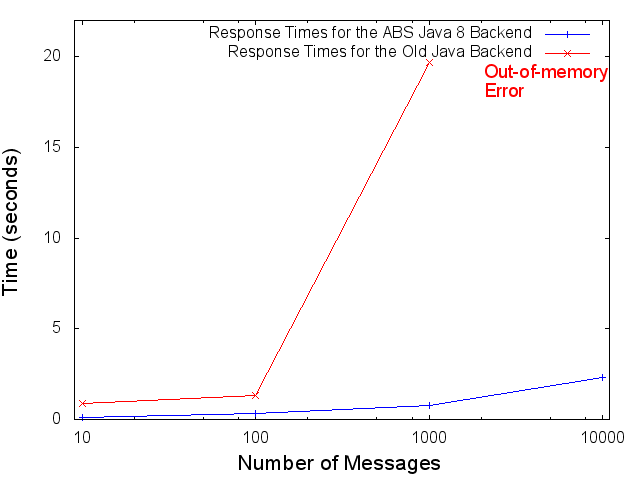
\includegraphics[scale=0.40]{./pictures/absj8t.png}
%	\caption{Old vs Java 8 Backend for ABS}
%	\label{abs8:ex}
%\end{minipage}
%\end{figure}

%\RH{Please get rid of white space in Fig.~\ref{abs8:ex} and reduce
%  distance between data points to shrink it horizontally, and also
%  vertically, so it fits in the minipage.}

%\begin{figure}[t]
%	\centering
%	\begin{subfigure}[b]{0.43\linewidth}
%		\label{abs8:cd}
%		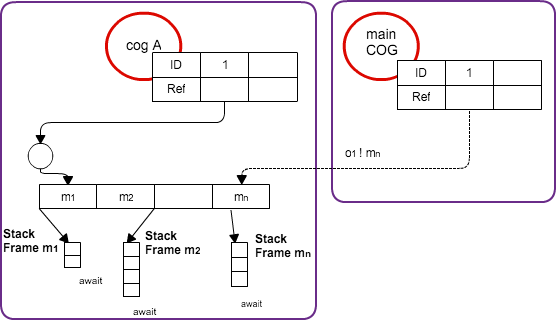
\includegraphics[scale=0.1]{./pictures/scenarioj8.png}
%		\caption{Scenario }
%	\end{{subfigure}
%	\begin{subfigure}[b]{0.50\linewidth}
%		\label{abs8:ex}
%		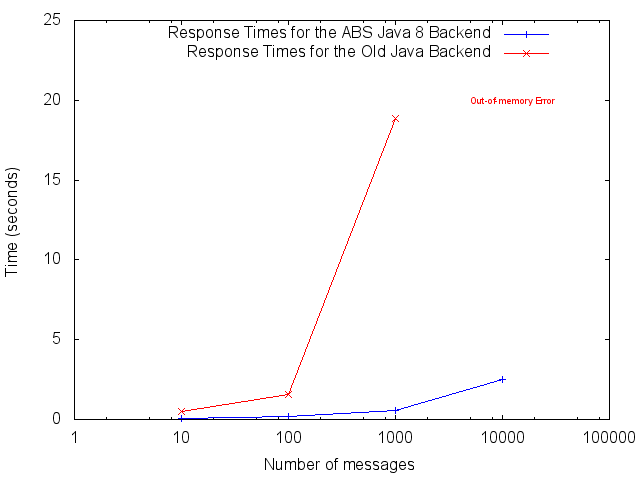
\includegraphics[scale=0.1]{./pictures/absj8ex.png}
%		\caption{Perfomance figures}
%	\end{subfigure}
% \caption{ABS Cooperative Scheduling Scenario and results}
 %\label{abs:comp}
%\end{figure}


%\begin{figure}
%	\label{abs8:cd}
%	\centering
%	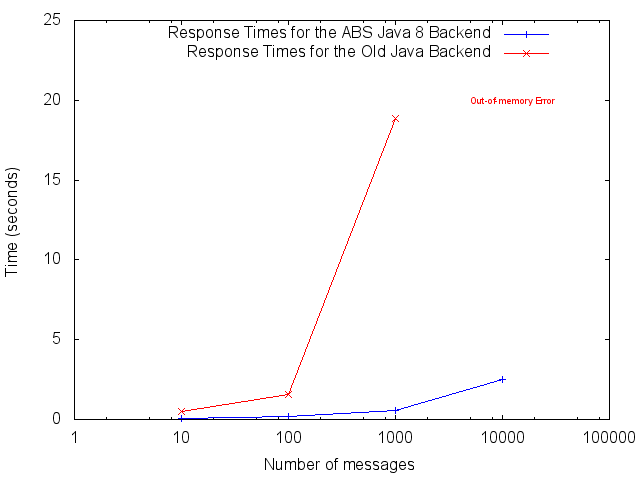
\includegraphics[scale=0.6]{./pictures/absj8ex.png}
%	\caption{Perfomance figures of the Two Java Backends for Cooperative Scheduling}
%\end{figure}

%When running on the previous Java backend, a series of 10000 calls on
%the same object requires immediate creation of a corresponding number
%of threads, resulting in the program running out of memory. This makes
%ABS unusable for HPC and Big Data applications that want to benefit
%from cooperative scheduling. While the Java 8 backend clearly performs
%better by minimizing the number of live threads at runtime, the
%challenge to handle cooperative scheduling of a large number of
%messages that are suspended and \emph{not} released remains an open
%research question.

\subsection{ProActive}
\label{sec:implem-proactive}

The ProActive library\footnote{Available at \url{https://github.com/scale-proactive}} is
completely written in standard Java and provides an
implementation for the ASP programming model targeting distributed applications.  By
default, it uses
 Java's remote method invocation package to implement the communication
layer between active objects, although other communication protocols
are possible.  This fact accounts for most of the implementation
specifics mentioned below.

\paragraph{Thread creation and scheduling}

In ProActive, an active object with no defined compatibility rule will
be associated with a single Java thread to process the requests.
Furthermore, there is a Java thread to handle request reception in
each active object.  Java threads are mapped to operating system
threads, thus ProActive uses at least two threads per active object.
But as ProActive features multi-active objects, this number can be
higher, as the active object scheduler can create Java threads on the
fly to process a compatible request.  Since Java threads are rather
heavy, the ProActive scheduler implementation makes a particular
effort in optimizing thread usage.  First, a thread pool is
instantiated at active object startup to ensure a basic thread reuse
policy.  Second, when the number of threads is limited at the
application level (through multi-active object annotations), that
limit literally maps to Java threads, such that fine performance
tuning can be achieved at the application level.  In addition, threads
waiting for a future can be temporarily reused to process the request
that will indirectly resolve the awaited future. This can be done
during wait-by-necessity.  To summarize, in ProActive thread creation
and thread scheduling are almost completely exposed to the programmer,
allowing him to have far ranging control over the performance of
ProActive applications.

\paragraph{Data sharing and object referencing}

Like ASP, ProActive differentiates between active and passive objects
in a way that is mostly transparent to the programmer, except that
passive objects are passed by copy when communicated between active
objects, while references between active objects can be shared and
accessed from anywhere.  The first reason for this behavior is that
ProActive is based on Java RMI, which in turn is based on parameter
copy.  The second reason is distribution: provision of a consistent
distributed memory is too costly for HPC, which is the primary target
of ProActive.  Of course, data is shared between the several threads
of a multi-active objects.

This sharing pattern is thus naturally implemented using RMI and Java
serialization performing a deep copy of the parameters transmitted
between objects. Future and active objects are implemented by a proxy
that can be passed by reference and is serialized as a reference
(without any copy of other referenced objects). The serialization
mechanism is also used to track multiple references to the same future
and to implement efficient future update
strategies~\cite{HKRZ:Coregrid:2010}.

Remote objects in RMI are globally referenced in what is known as the
RMI registry: a mapping from remote object names to remote object
stubs that can be copied and used anywhere to access the remote
object.  Networking communication is ensured by the RMI-JRMP protocol.
Consequently, all active objects in ProActive are referenced in an RMI
registry and can be accessed in this way from any other object through
the adapted protocol.  For non-active objects, traditional Java object
references are used as they are only referenced within the same active
object.  To summarize, two types of object references exist in
ProActive: global references, retrievable from the RMI registry, and
local references, acting like standard reference types.

\paragraph{Error handling}

Distributed environments are prone to failures.  Since ProActive
targets distributed environments, a particular effort was made in
producing robust ProActive applications by design.  To this end, the
ProActive library includes two error handling mechanisms.  First, an
exception chaining mechanism was developed on top of
\texttt{RemoteException}, the basic RMI exception, in order to obtain
readable feedback when ProActive applications crash. Second, a
specific API has been developed to compensate for the difficulty of
dealing with asynchronous exceptions and the lack of control over the
Java exception mechanism~\cite{CC-ECOOPWS2005}.

A further aspect of the ProActive library concerns continuing to
execute an application in presence of failed active objects, for
example, when a machine hosting an active object of the application
crashes.  For this purpose ProActive implements a fault tolerant
protocol specific to the active object semantics. It enables a set of
failed active objects to restart from the latest checkpoint.
Checkpoints are recorded per active object, based on the
communications between them.  This strategy is coupled with the
logging of events received by the active object to ensure a
deterministic reexecution.  The fault tolerant protocol is complete
for applications that only feature mono-threaded active objects.  It
is under development for applications that feature multi-active
objects.

\paragraph{Garbage collection}

Handling garbage collection in ProActive is deeply linked with how
objects are referenced.  No particular mechanism is needed to ensure the
garbage collection of regular objects, because the Java garbage
collector will take care of that.  Since a regular object cannot be
referenced by more than one active object, it is guaranteed that no
reference to this object exists in another JVM, hence, standard
garbage collection suffices.  However, for an active object, we cannot
directly know whether a reference to it still exists, because many
proxies to it can be disseminated throughout the network.  An adapted
algorithm to garbage collect active objects was developed in
ProActive.  It is based on the detection of useless active objects
(those that are idle and only referenced by idle active objects). This
is detected as a form of common agreement based on the reference graph
between active objects~\cite{CCH:Middleware07}.

\subsection{ProActive Backend for ABS}
\label{subsec:proactive-backend-abs}

The ProActive backend for ABS\footnote{Available at:
\url{https://bitbucket.org/justinerochas/absfrontend-to-proactive}} generates ProActive
code corresponding
to an ABS program~\cite{rochas:hal-01065072}. The goal of the
ProActive backend is to provide a fully working execution of ABS
models in distributed environments, with less optimization than
necessary for the Java 8 backend. Since the two languages are based on
different active object models, the main challenges in the translation
are (i) how to efficiently support object groups in ProActive where
only active and passive objects are available, (ii) how to handle
objects in the translation since objects are passed by reference in
ABS and by copy in ProActive, and (iii) how to simulate cooperative
scheduling with multi-threading controlled through annotations. We
first present object referencing aspects, because the scheduling depends
on the set of objects classified as active.

\paragraph{Data sharing and object referencing}

All objects in ABS are accessible from all others (via suitable
getter/setter methods); thus, one could implement each ABS object with
a ProActive active object. In practice, this is infeasible: a
ProActive active object has an associated plain Java thread. So this
solution would inevitably lead to substantial memory consumption and
context switch overhead.  Instead, in the code generated by the
ProActive backend only COGs are active objects and serve as the entry
point to all objects they contain.  This hierarchy implies that other
objects than COGs are passive, preserving the performance of the
ProActive backend.  Thus, on the first level of the index hierarchy we
have network-wide accessible COG objects. That mechanism is integrated
in ProActive, as it is based on RMI.  At the second index level we
have locally accessible objects. That mechanism is implemented in the
COG class with a map from object identifiers to object references.
The translation introduces indirection through COGs that are
accessible by remote reference.  This configuration of objects is
illustrated in Fig.~\ref{fig:ABS-to-PA-new}, where a COG 2 is created
through a new \code{Server} object.

\begin{figure}[t]
		\begin{subfigure}[b]{0.43\linewidth}
                 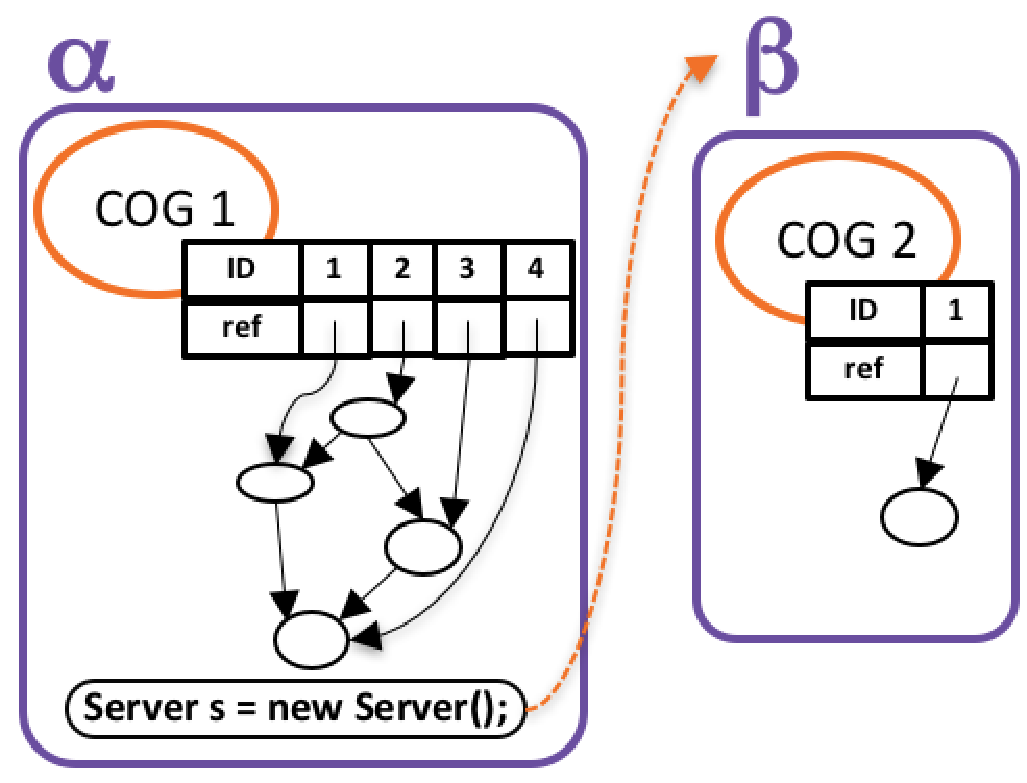
\includegraphics[scale=0.3]{pictures/ABS-to-PA-new.pdf}
                \caption{ABS new in ProActive}
                \label{fig:ABS-to-PA-new}
        \end{subfigure}
        \begin{subfigure}[b]{0.50\linewidth}
                  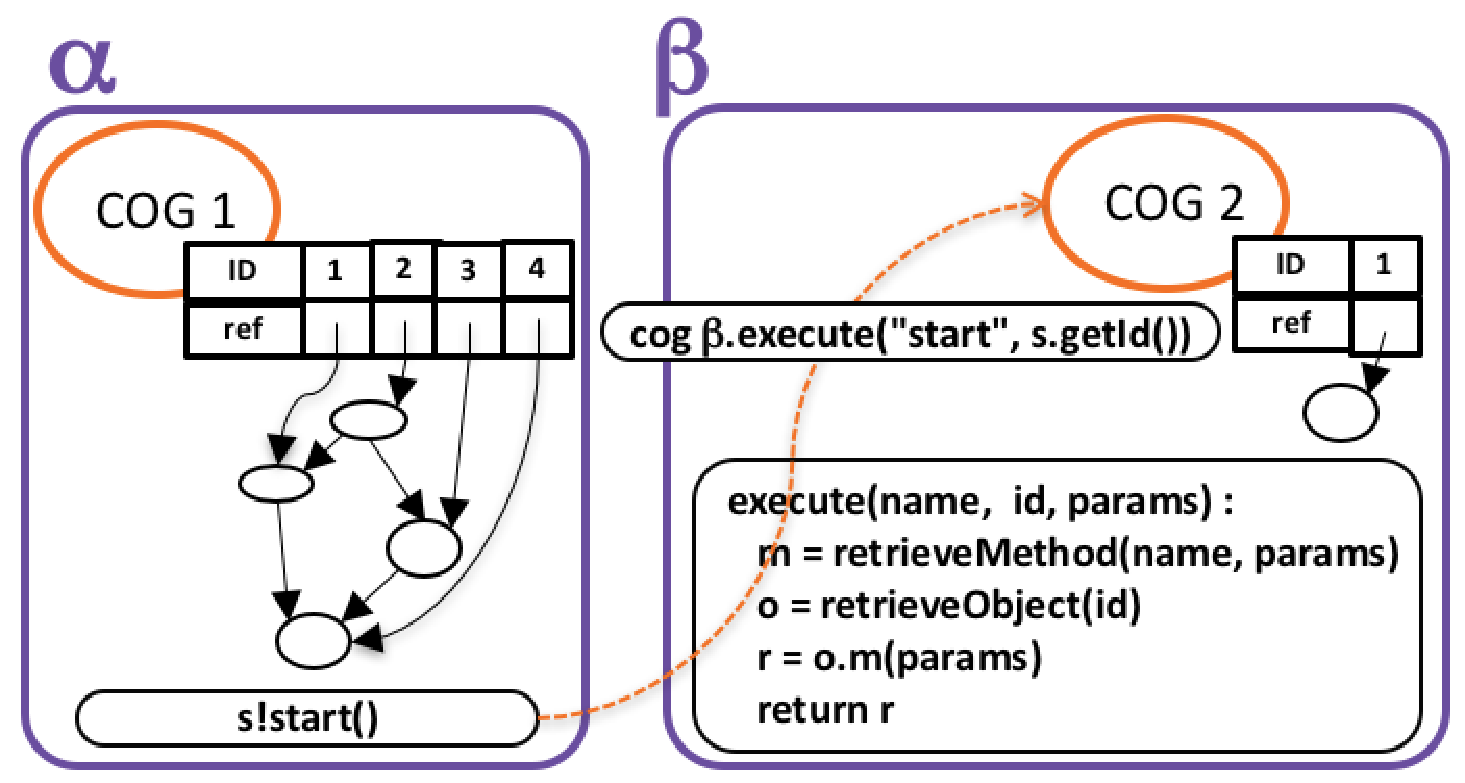
\includegraphics[scale=0.3]{pictures/ABS-to-PA-call.pdf}
                \caption{ABS asynchronous method call in ProActive}
                \label{fig:ABS-to-PA-call}
        \end{subfigure}
 \caption{Representation of ABS objects and calls in ProActive}
\label{fig:graph}
\end{figure}

%\begin{figure}
%	\centering
%	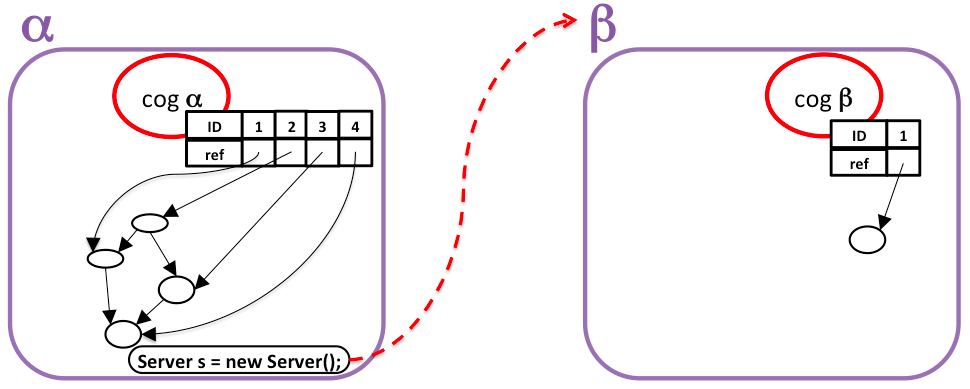
\includegraphics[scale=0.3]{pictures/ABS-to-PA-new.png}
%	\caption{Object organization given by the ProActive backend for ABS when a new COG is created}
%	\label{fig:ABS-to-PA-new}
%\end{figure}

An  asynchronous  call in ABS is
translated into a generic asynchronous method call on the COG serving as the index to the targeted
object. Then a generic caller method of the COG  retrieves the targeted object
via a unique
identifier and runs the desired method on it using reflection, see
Fig.~\ref{fig:ABS-to-PA-call}.
%\begin{figure}
%	\centering
%	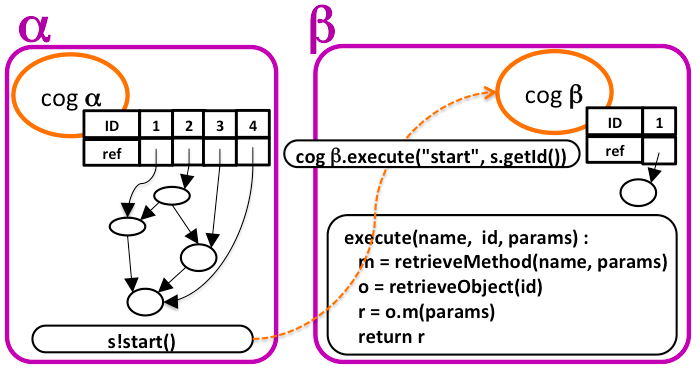
\includegraphics[scale=0.3]{pictures/ABS-to-PA-call.png}
%	\caption{Translation of an ABS asynchronous method call in ProActive}
%	\label{fig:ABS-to-PA-call}
%\end{figure}
In ProActive passive objects are not shared between active
objects. Therefore, a passive object is copied when it is a parameter
of a remote method call, whereas parameters of method calls in ABS are
passed by reference.  When the translation performs a remote method
call on a COG, all parameters get copied. This is not a problem for
the identifier of the targeted object, the name of the method to run,
and the primitive values, because they are immutable. For the
reference type parameters the differing parameter passing semantics is
still safe, but for a different reason.

While any access to an object is via an asynchronous method call on
the copy of method parameters, those invocations end up calling the
unique original version of the created object and their hosting
COG. Thanks to this mechanism, data sharing in ABS is correctly
simulated under the no-sharing philosophy of ProActive, because the
copied data is only used as a reference to the original object.  This
means that, when we copy an object from one node to another, we only
need the object's identifier plus a reference to its COG to retrieve
it in the right memory space. Its other attributes can be omitted.
This observation allows to optimize object copying and saves
bandwidth. Consequently, the ProActive backend generates programs that
copy less data but incur more communication than native ProActive
applications. Compared to the Java 8 backend for ABS, the ProActive
backend does not distinguish whether COGs are located on the same
machine to optimize communication, however, this is not a problem
since only references are copied.  Also, in the ProActive backend
class loading is handled by RMI, whereas it is implemented from
scratch in the Java~8 backend.

\paragraph{Thread creation and scheduling}

Multi-active objects provide several mechanisms to control the
scheduling of requests. Their proper tuning allows the ProActive
backend to simulate the behavior of ABS cooperative scheduling.  When
comparing the ProActive backend and the Java 8 backend
(Section~\ref{sec:implem-java-8}), we can state that both deliver one
message per asynchronous invocation, but in ProActive a single request
queue exists for all objects in a same COG, whereas in the Java 8
backend, there is one request queue per object.  The Java 8 backend
ensures that all objects in the same COG compete for one single
thread, whereas the ProActive backend creates one thread per executing
(and paused) request: it is the scheduling derived from compatibility
annotations that ensures at most one request is progressing at a
time. This strategy avoids continuations which are difficult to
implement in Java, because of JVM restrictions. Finally, the Java 8
backend shares a thread pool for many COGs whereas in the ProActive
backend each COG has its own thread pool.  To summarize, the ProActive
backend has to handle more idle threads than the Java 8 backend.

% We explain below in more details how we implement ABS preemption
% constructs in ProActive.

% More precisely, we can compare the ProActive backend and the Java 8 backend  on the four
% points explained in Section~\ref{sec:implem-java-8}. On points 1 and 3, the ProActive
% backend also delivers a message per asynchronous invocation, but a single request queue
% exists for all objects in a same COG, whereas in the Java 8 backend, there is a request
% queue per object. Concerning point 2, the Java 8 backend ensures that all objects in the
% same COG compete for one single thread, whereas the ProActive backend creates one thread
% per executing (and paused) requests: it is actually the scheduling associated to
% compatibility annotations that ensures that only one request is progressing at a time;
% this strategy avoids implementing continuations in Java which is difficult because of JVM
% constraints. Finally, on point 4 the Java 8 backend shares a thread pool for many COGs
% whereas in the ProActive backend each COG has its own thread pool. In conclusion, the
% ProActive backend has to handle more idle threads than the Java 8 backend. We explain
% below in more details how we implement ABS preemption constructs in ProActive.
%\RH{I removed the references to points 1--4, because they don't appear
%  in Section~\ref{sec:implem-java-8}, which is confusing. Copy of
%  original text is preserved, but commented out.}

The central idea to implement ABS preemption in ProActive is to
exploit thread limits: a hard limit restricts the total number of
threads for a multi-active object instance, a soft limit merely
restricts the number of active threads.  Now we first declare the
generic caller method of a COG that executes all other methods to be
compatible with itself, i.e., many activations of such methods are
allowed to run in parallel. Then we impose on this set of methods a
soft thread limit of one.  Hence, there is at most one active thread
at any time that serves requests in a COG multi-active object.
Requests do not run in parallel but interleave using
wait-by-necessity: \lstinline{await} on a future is translated into
access to a future, that frees the current active thread (soft limit).
Blocking \lstinline{get} statements are also translated to future
accesses, but the current active thread is not released (a hard limit
is ensured).

This work highlights the differences between the two languages,
especially regarding futures. In ProActive the synchronization is
\emph{data-flow oriented} as futures are transparently accessed and
updated, and wait-by-necessity can only be released upon access to
some data. In ABS synchronization on future is \emph{control-flow
  oriented}: a future access succeeds upon request
termination. However, in most programs a future access is used to
retrieve information and the control-flow synchronization of ABS
corresponds to a data-flow synchronization; however, syntactically,
there exist programs that do not behave the same.  We have formally
proven~\cite{rochas:hal-01065072} that all ABS programs are faithfully
simulated by the ProActive backend; the proof highlights the
differences between the future access semantics of the two languages.

% \smallskip
% $\bullet$ \textit{Translation of  \code{await} statement on futures.}
% %% RM
% With multiactive objects, a way to control what happens when a thread switches in
% wait-by-necessity is to specify the kind of thread limit: a hard limit restricts the
% total number of threads existing for a multiactive object instance whereas a soft limit
% only restricts the number of threads that are active (not in wait-by-necessity).
% To achieve the request scheduling of ABS, we  declare that the generic method of the COG
% that executes all methods by reflection is
% compatible with itself, which means that many of such methods are allowed run in
% parallel. Additionally, this set of methods has a thread limit of 1, with a soft limit.
% Thus, there is only one active thread at a time that
% serves requests in a COG multiactive object: requests do not run in
% parallel but interleave upon wait-by-necessity.
% %Consequently, this multiactive
% %configuration leads to a similar scheduling as ABS.

% \smallskip
% $\bullet$ \textit{Translation of  \code{get} statement.}
% %The translation of the ABS \code{get} statement would have been straightforward if we
% %had
% %not configured the COG class for the translation of the \code{await} statement. Indeed,
% %by doing so,
% The problem  is that
% we have disabled the blocking aspect of a ProActive wait-by-necessity to handle
%  cooperative thread release upon await statement.
% Consequently, to translate the \code{get} statement we temporarily go back to the initial
% behavior of a ProActive wait-by-necessity and switch the thread limit to a hard thread
% limit so that no
% other request can execute while the get statement is executed.
% %When the future is resolved,
% %we set back the soft limit restore the cooperative scheduling behavior.
% %% RM

% \smallskip
% $\bullet$ \textit{Translation of  \code{await} statement on conditions.}
% To handle an \code{await} statement on a condition we generate a  method and create an
% asynchronous request (of another compatible group) that checks the condition ane finishes
% when the condition is verified. It is then sufficient to perform an await on the future
% for this request as explained above.
% %Another usage of the ABS \code{await} statement is to use it followed by a condition.
% %For
% %translating this kind of \code{await} in ProActive, we wrap the condition evaluation in
% %a
% %method call that returns a future, and we synchronize on it afterwards. More precisely,
% %for each such condition, we generate a corresponding method. Then, we translate the
% %\code{await} statement by an asynchronous call to another generic method of the COG
% %class
% %that is specially devoted to execute waiting conditions, giving it all required
% %parameters to do that. Again, we configure this method with multiactive annotations in
% %order to allow several conditions to run in parallel.
% %We allocate many threads for the evaluation of conditions and reserve through
% %annotations
% %one thread for the generic method execution.
% %%% RM
% %This way, we have a clear separation between the single thread used by application
% %method, and the threads used by the condition execution method.
% %%% RM
% \smallskip

%\RH{I have shortened the explanation to the paragraph above, which to
%  me, seems detailed enough. Please check. Original text is just commented out.}


%%%% Without the figures, the text could be like the one below %%%%
%In addition, we have performed two experimental evaluations on an ABS
%application translated with the ProActive backend, that show that (i) the translated
%application run in a distributed environment indeed outperforms traditional ABS program
%execution, and (ii) that the overhead introduced by the translation is always kept under
%10\% compared to a native ProActive application.

\paragraph{Example and experiments}
We use a representative HPC application, pattern matching of a DNA
sequence programmed in the MapReduce
model~\cite{Dean:2008:MSD:1327452.1327492}. The case study is
computation-intensive and relies less on active object communication
than the experiment reported in Section~\ref{sec:implem-java-8}. As
ProActive relies on physical threads for active objects and data
copying occurs in each communication, ProActive is better suited for
computation-intensive scenarios than for communication-intensive ones.
We compared performance of the code generated with the ProActive
backend~\cite{rochas:hal-report} for ABS run in distributed mode, the
code generated with the Java 8 backend of ABS run on a single
machine, and native code written manually in ProActive for the same algorithm.
%
Map instances (workers) are created in their own COG.  We search a
pattern of 250 bytes inside a database of 5 MB. Each map searches for
the maximum matching sequence of a chunk and a reducer outputs the
global maximum matching sequence.  We report the global execution
time. When deploying with ProActive, we instantiate two workers on each machine (each
machine has two dual-core CPUs). In the generated
program, we manually replaced the translation of functional ABS types
(integers, booleans, lists, maps) with standard Java types, similar to
the code the Java 8 backend produces.
% All used machines have 2 dual core CPUs at 2.6GHz, and 8 GB of
% RAM\footnote{We use a cluster of Grid5000 platform:
% \url{http://grid5000.fr}}.

\begin{figure}[t]
		\begin{subfigure}[b]{0.50\linewidth}
                 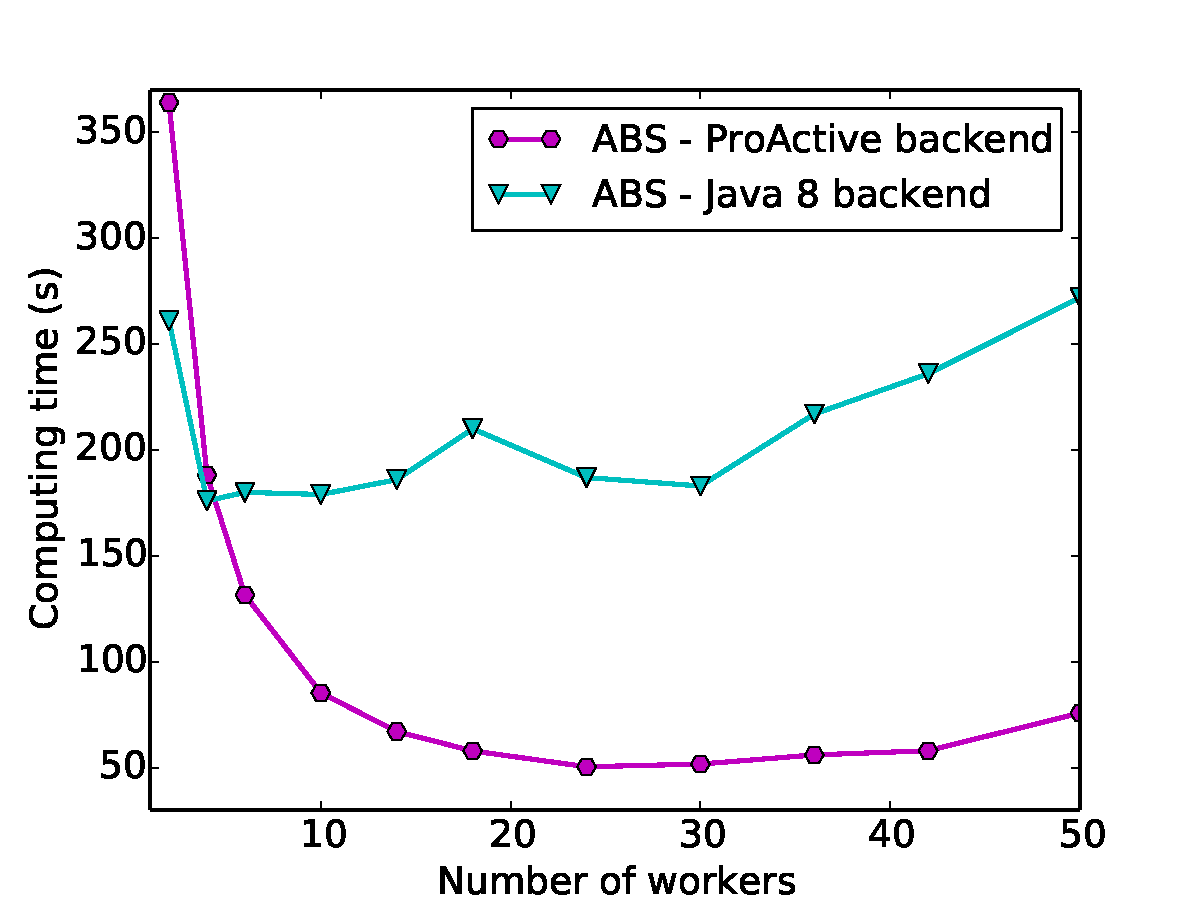
\includegraphics[scale=0.31]{pictures/usecase-pa-java-8.pdf}
                \caption{ProActive backend vs. Java 8 backend}
                \label{fig:bench-usecase}
        \end{subfigure}
        \begin{subfigure}[b]{0.50\linewidth}
                  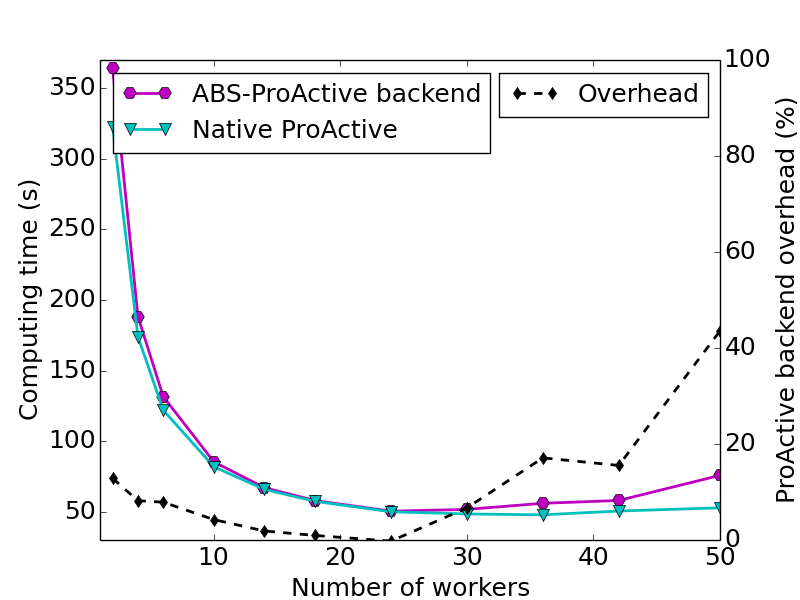
\includegraphics[scale=0.31]{pictures/native-finalV2.png}
                \caption{ProActive backend vs. native ProActive code}
                \label{fig:bench-native}
        \end{subfigure}
 \caption{Execution time of DNA-matching ABS application}
\end{figure}

Fig.~\ref{fig:bench-usecase} shows the execution times of both ABS
backends for the application ranging from 2 to 50 workers, using from
1 to 25 physical machines with ProActive.  The execution times of the
ProActive backend are sharply decreasing for the first few added
machines and then decrease at a slower rate. The first instance added in the Java 8
backend also improves significantly the performance of the program and the Java 8 backend
performs better with one or two workers. Then, thanks to the
efficient thread management of the Java 8 backend, the performance stays stable until 30
workers. Finally with a high number of instances the degree of parallelism becomes
harmful.  In contrast to
this, increasing the degree of parallelism for the ProActive backend
results in a linear speedup, because it balances the load between
machines and benefits from distribution.

Figure~\ref{fig:bench-native} compares the performance of the
generated ProActive code to a hand-written version.
% Indeed, our point here was to evaluate the additional communication
% cost of our translation, not the performance of ABS types compared
% to standard Java types.  \footnote{As can be noticed on the
% generated ProActive of Figures~\ref{fig:bench-usecase}
% and~\ref{fig:bench-native}, there is an order of magnitude of
% difference depending on the types used; fixing this is
% on-going~\cite{ref:ABS-Java-translate}.}
The overhead introduced by the translation performed by the ProActive
backend is very low ($<10$\%), except when many machines are involved
and the communication rate is high.
% At the biggest stage, the application translated with the ProActive
% backend starts to have a higher overhead because it involves too
% much communication.

\subsection{Encore}\label{encore-implem}

The Encore implementation \footnote{Available at \url{https://github.com/parapluu/encore}}  consists of two major components, a
source-to-source compiler (from Encore to C) implemented in Haskell,
and the runtime system, implemented in C. The runtime provides efficient parallel
execution but has no support for distribution.  The Encore runtime stack
(Fig.~\ref{fig:encore:stack}) is built around the runtime used by the
 Pony language
(PonyRT) \cite{ClebschDBM15}, which includes an actor library and garbage collection for
both active objects (actors)~\cite{DBLP:conf/oopsla/ClebschD13} and
passive objects~\cite{clebsch2015ownership}. The Encore runtime
(EncoreRT) extends the PonyRT with new features such as futures, the
\parT{} abstraction, a task library, and the notion of \emph{encore
threads} (explained below). These features are part of the runtime and
are therefore written in C.  On top of these libraries rests the
Encore Standard Library, which is written in Encore itself.

\begin{figure}[t]
  \centering
  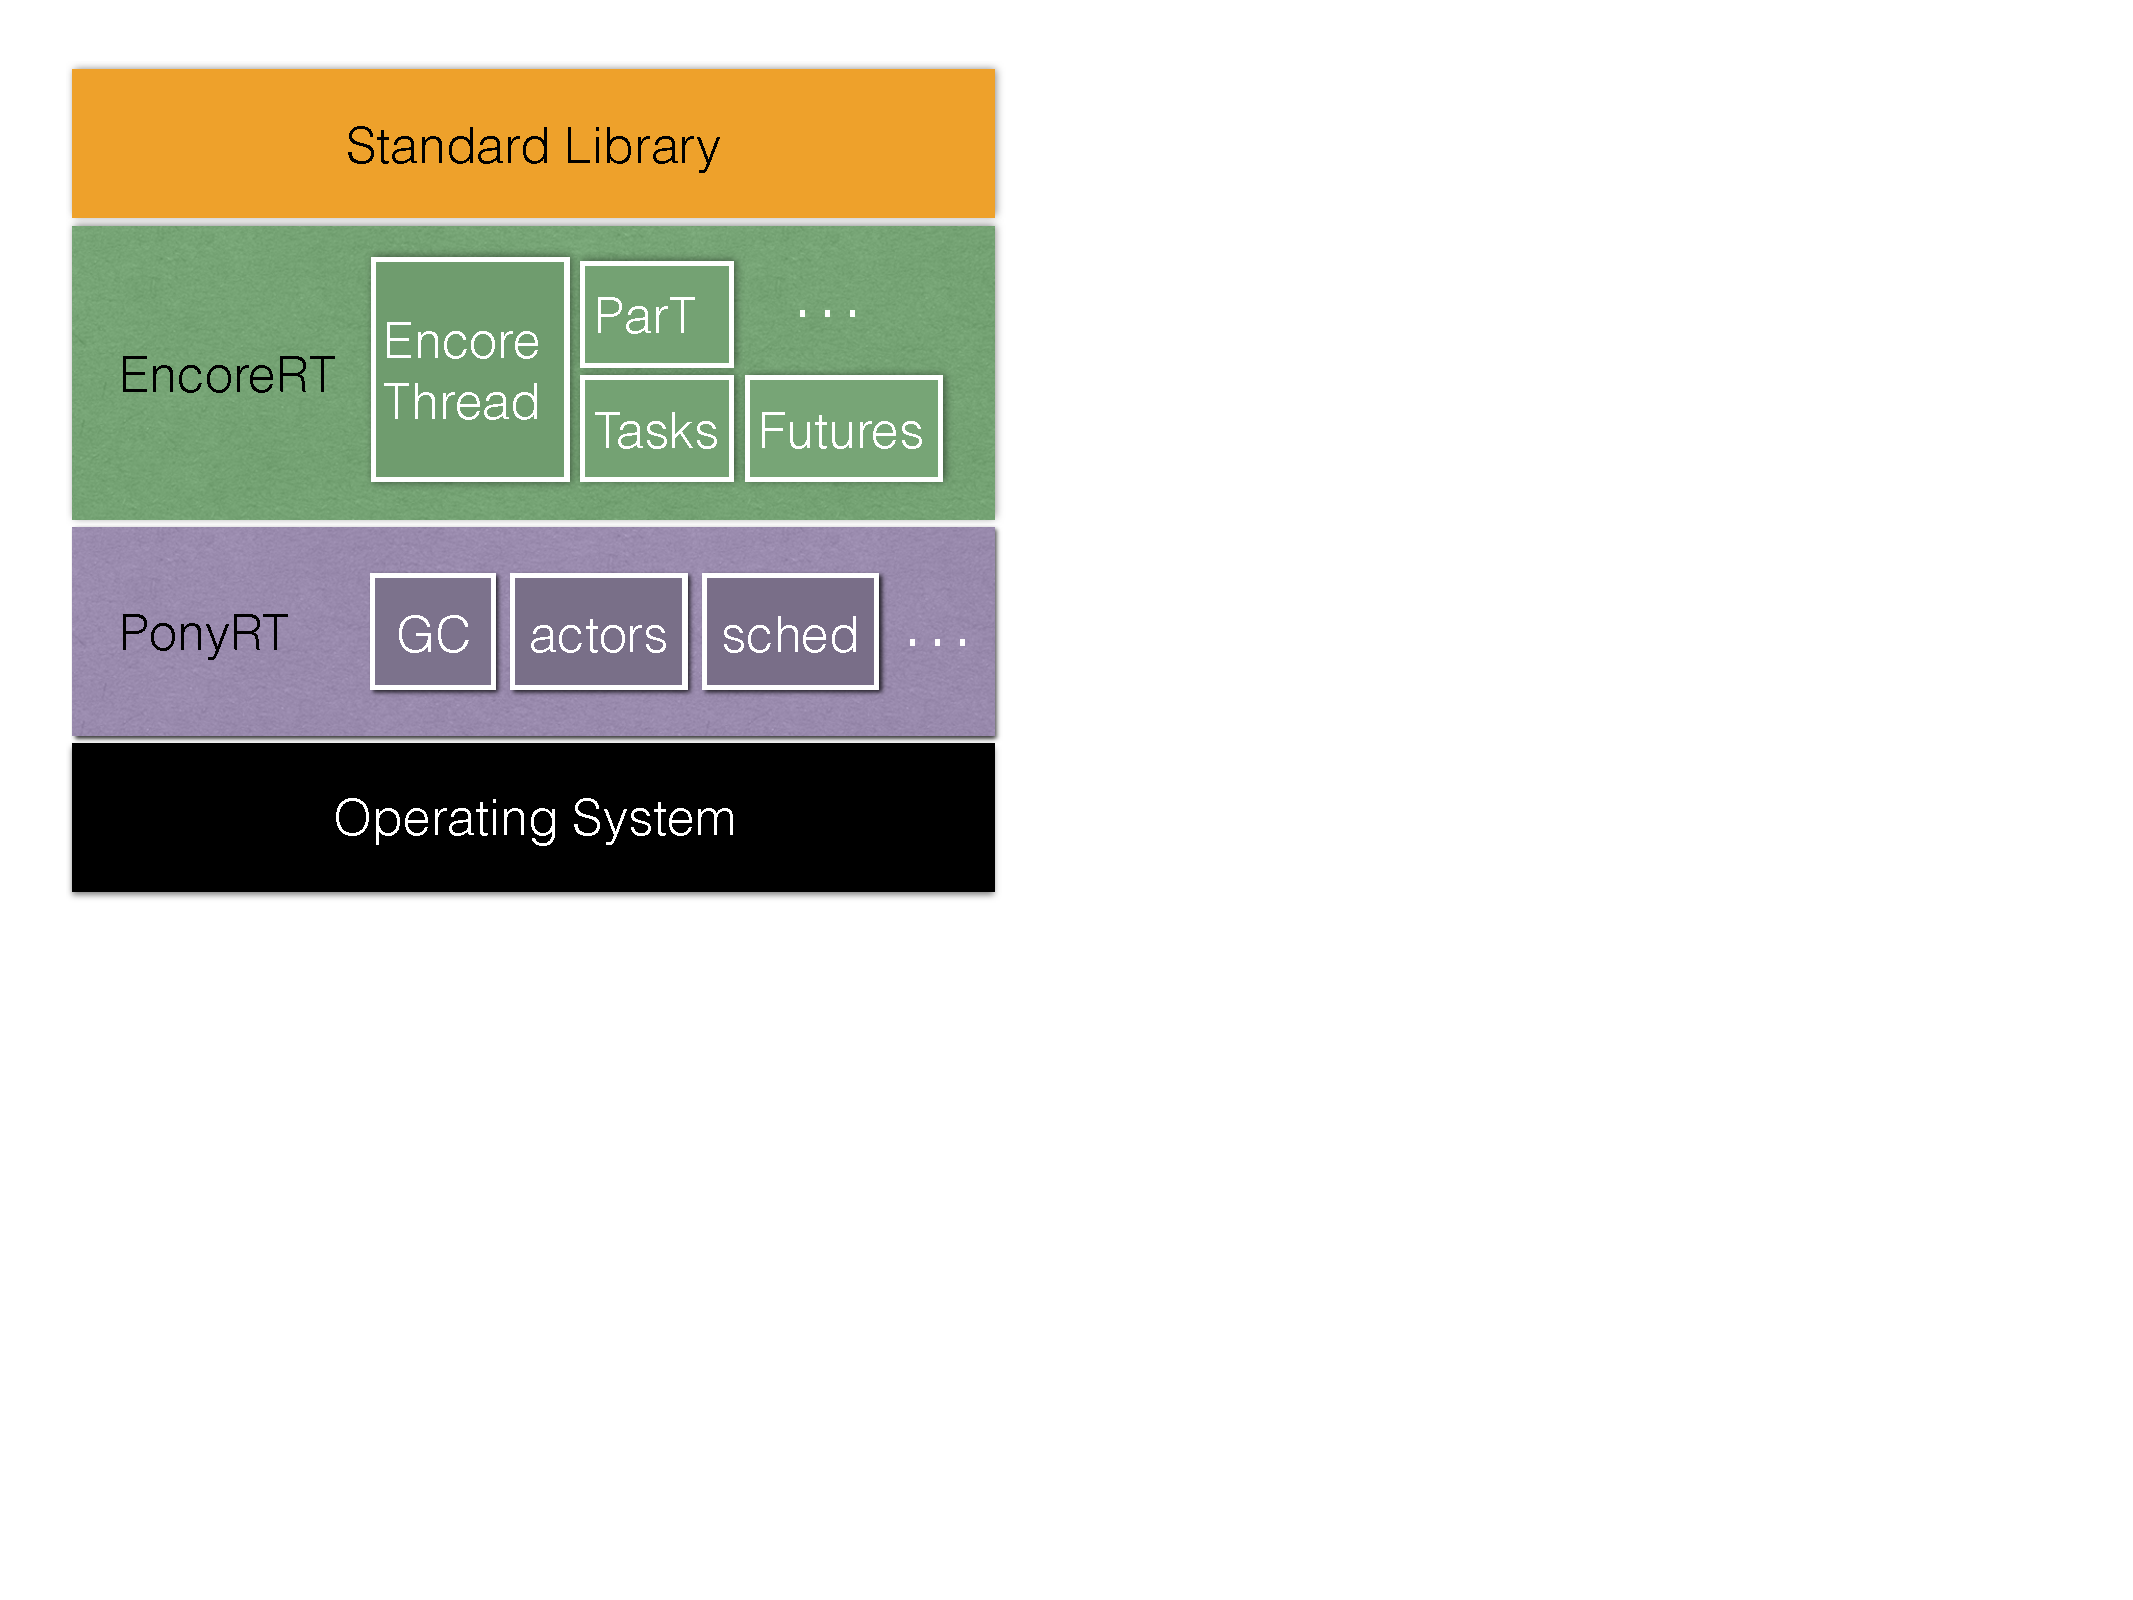
\includegraphics[width=2.5in, trim=0 4in 7in 0]{pictures/encore-stack}
  \caption{\label{fig:encore:stack} Encore Runtime stack}
\end{figure}


\paragraph{Thread creation and scheduling}

In Encore, the runtime has schedulers whose responsibility is to
schedule active objects. Each scheduler owns a queue of active objects
and each active object owns its own mailbox, which contains messages
to process.

On system start-up, the runtime maps physical cores to schedulers,
saving the overhead of creating and context switching over a large number
of threads, although this can be overridden if desired.
%
Each scheduler runs in a loop, scheduling active objects until the
whole program terminates. In each iteration of the loop, the scheduler
performs three procedures.  First, the scheduler pops an active object
from the beginning of the queue. Second, it hands over control to the
active object so that it can process messages in its mailbox. The
active object can only process one message at a time to ensure
fairness. Third, if a message is indeed processed in the previous
step, the active object is pushed to the end of the scheduler's queue;
otherwise, the active object is unscheduled due to having an empty
mailbox. Unscheduled active objects are rescheduled when other active
objects send messages to them. Furthermore, in the second step, new
active objects could be created, and they would be pushed to the end
of queue of the current scheduler.
%
Active objects can be migrated from one scheduler to another via work
stealing, which realizes a load balancer; this only happens when a
scheduler runs out of active objects.

Active objects in Encore are implemented by a lightweight abstraction
called \emph{encore thread}, which resembles green threads. Each
active object is assigned an \emph{encore thread} which provides a
thread-of-control to the active object, so that it can process
messages in its message queue.  This implementation detail makes
Encore capable of running thousands of active objects on the same
machine.

The semantics of \ec{suspend}, \ec{await}, and \ec{get} is illustrated
by Figs.~\ref{fig:enc-suspend} and \ref{fig:enc-get-await}, which show
how these operations involve \emph{descheduling} (removed from
round-robin scheduler queue) and \emph{blocking} (no processing of
other messages in the active object's queue) of an active object, and
whether a resuming message is prepended or appended to the active
object's message queue.

\begin{figure}[t]
	\centering
	\qquad
	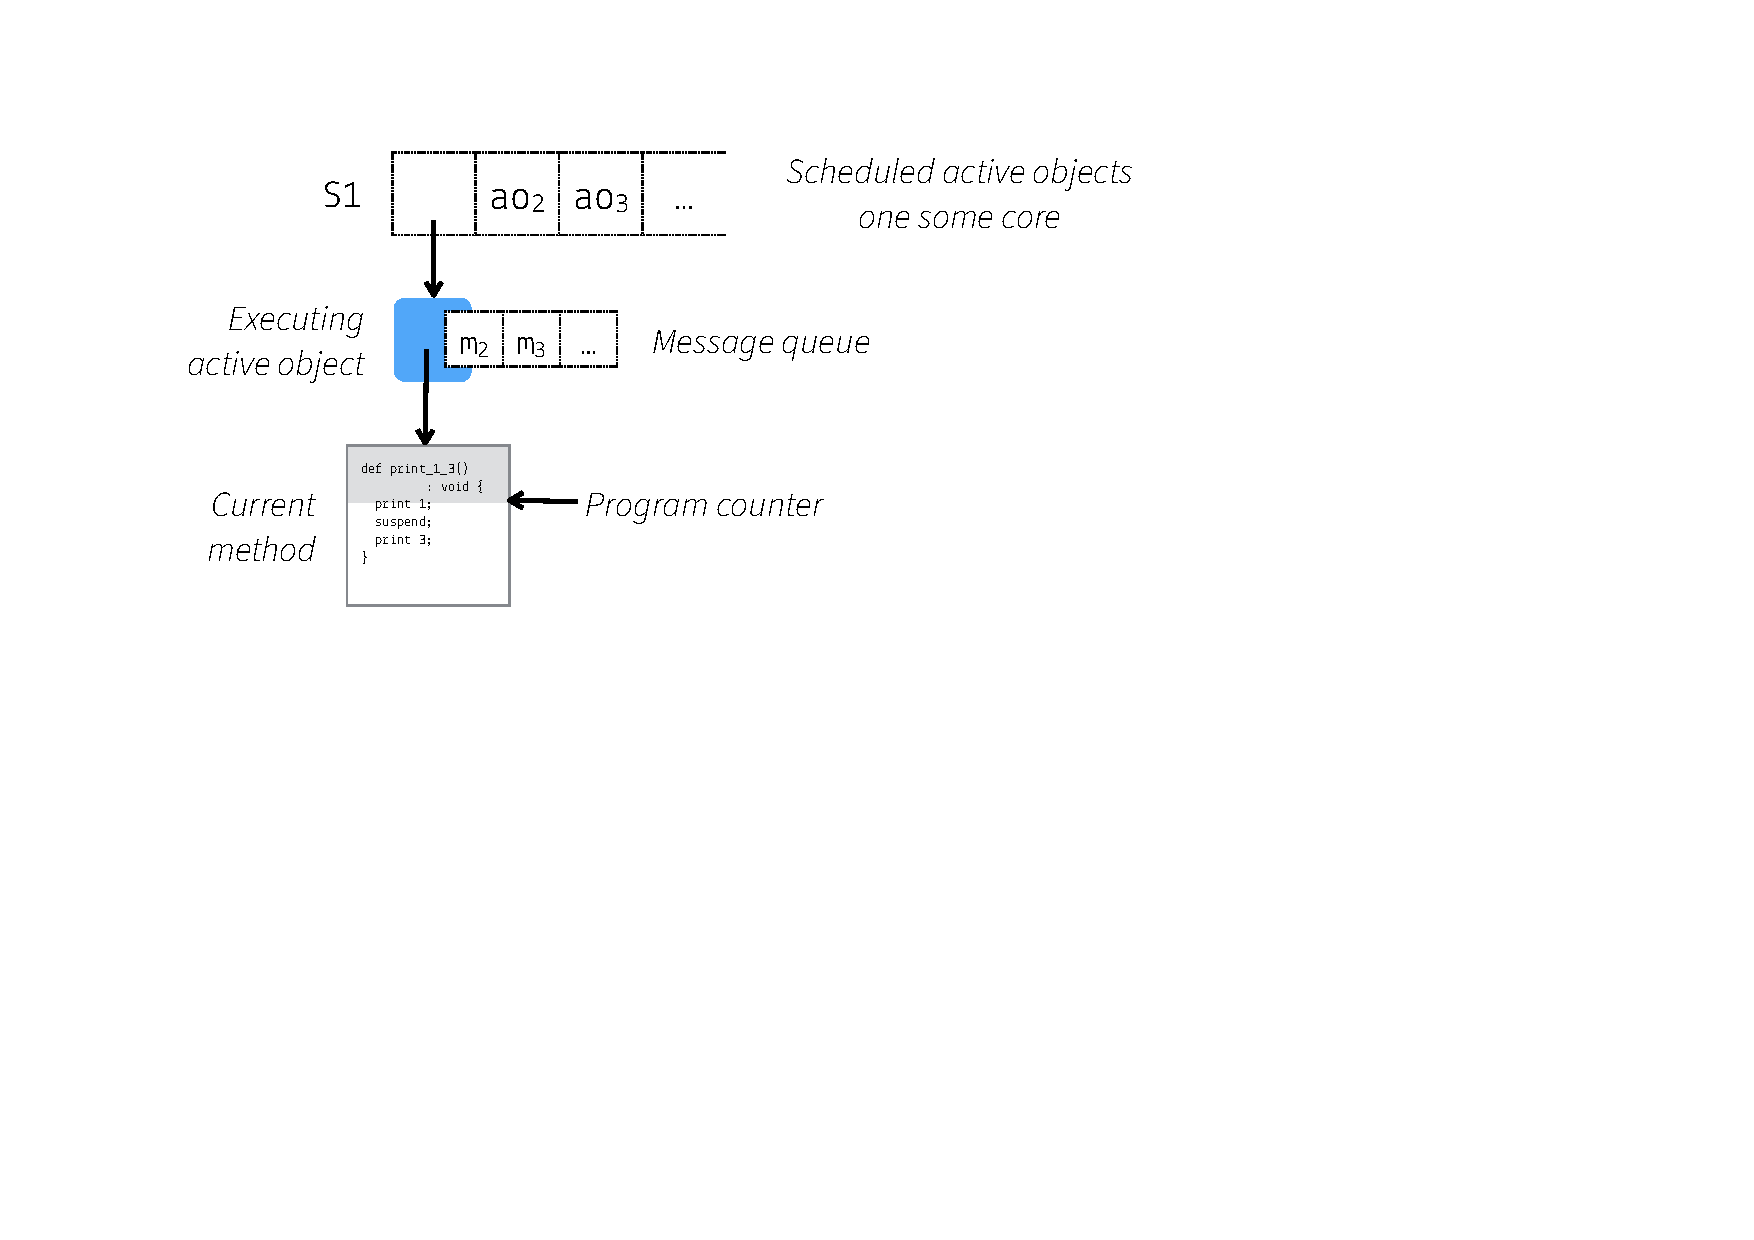
\includegraphics[scale=.45, trim=2in 4in 1in 4in]{pictures/enc-basic}
	\qquad
	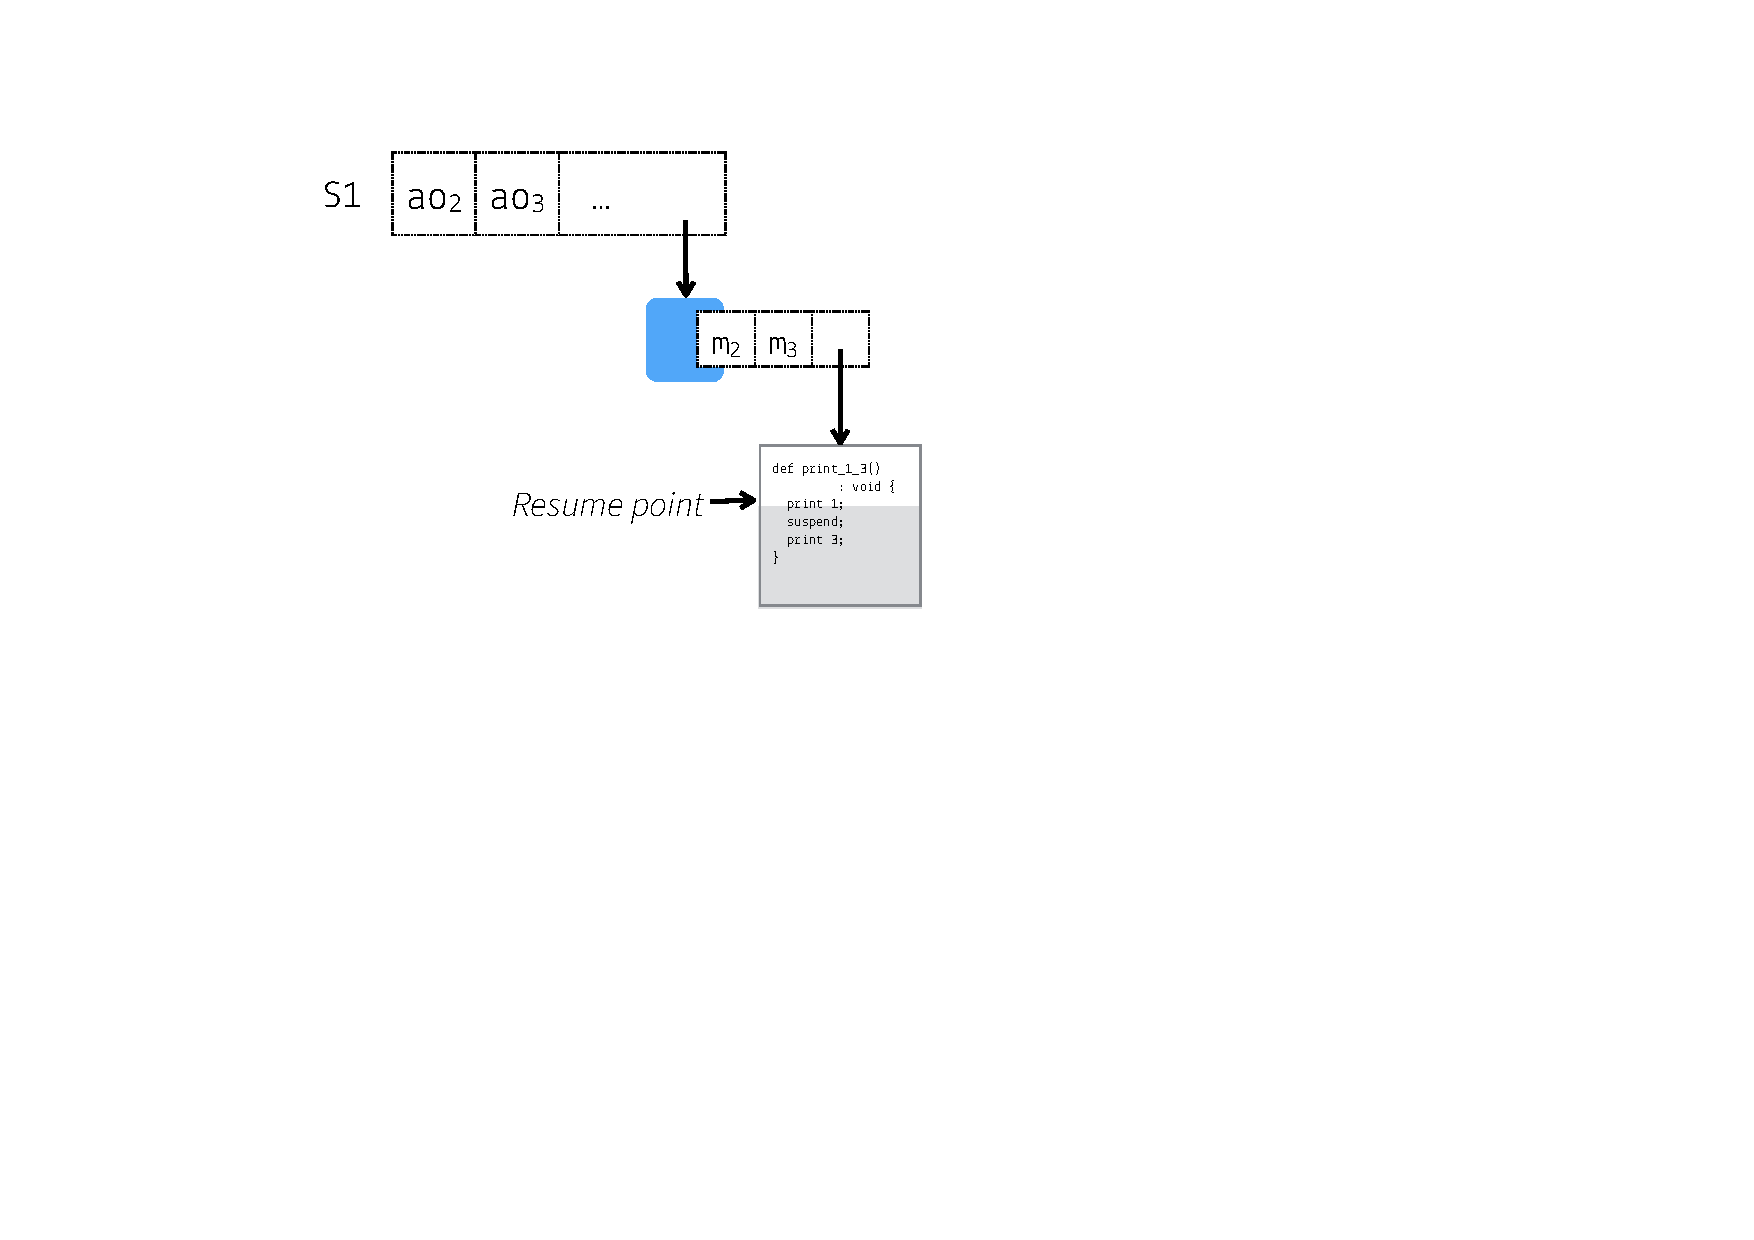
\includegraphics[scale=.45]{pictures/enc-resume}
	\caption{An Encore scheduler, local to one core. (\emph{Left})
          A scheduler has a queue of active objects with non-empty
          message queues. (\emph{Right}) The state after execution of
          \ec{suspend} in the left configuration.}
	\label{fig:enc-suspend}
\end{figure}

\begin{figure}[t]
	\centering
	%  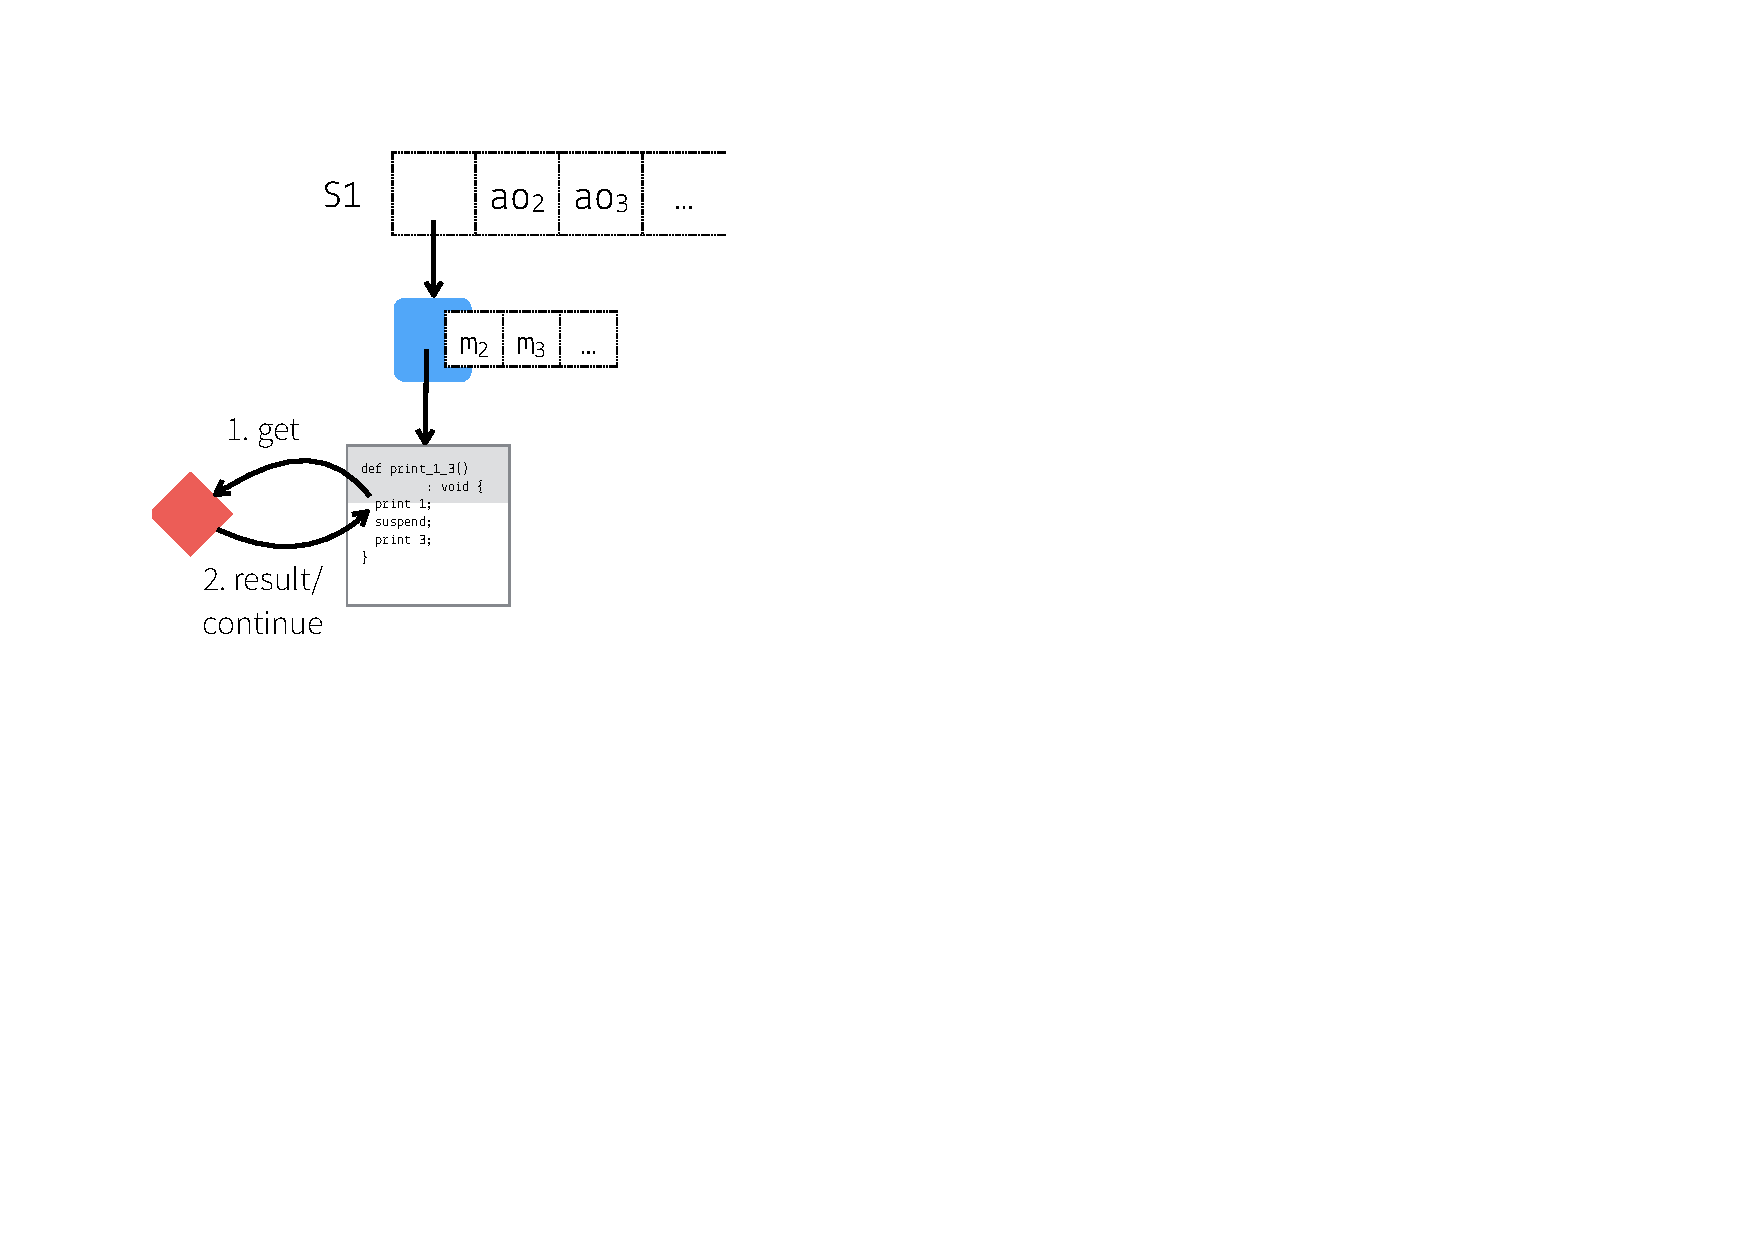
\includegraphics[scale=.4]{pictures/enc-get-await-fulfilled}
	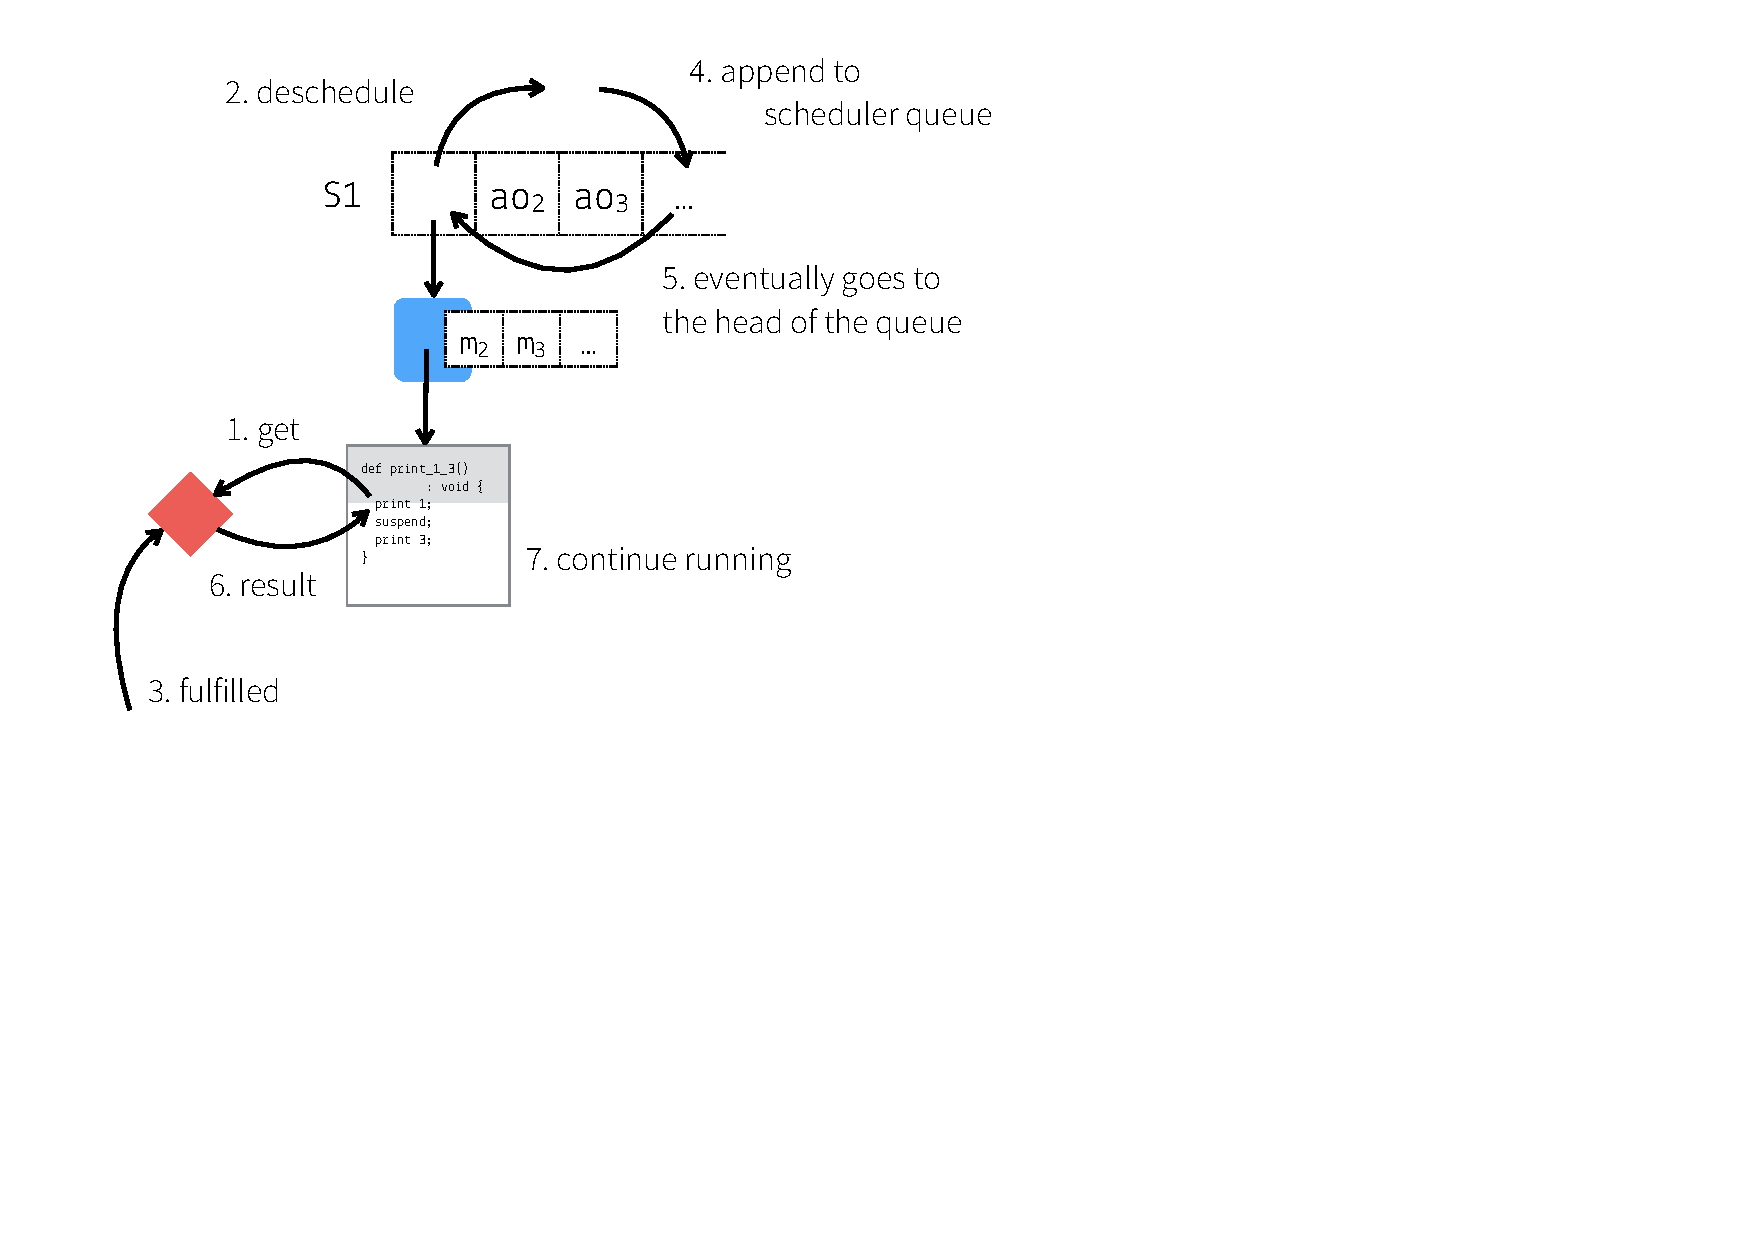
\includegraphics[scale=.42]{pictures/enc-get-unfulfilled}
%	\qquad
	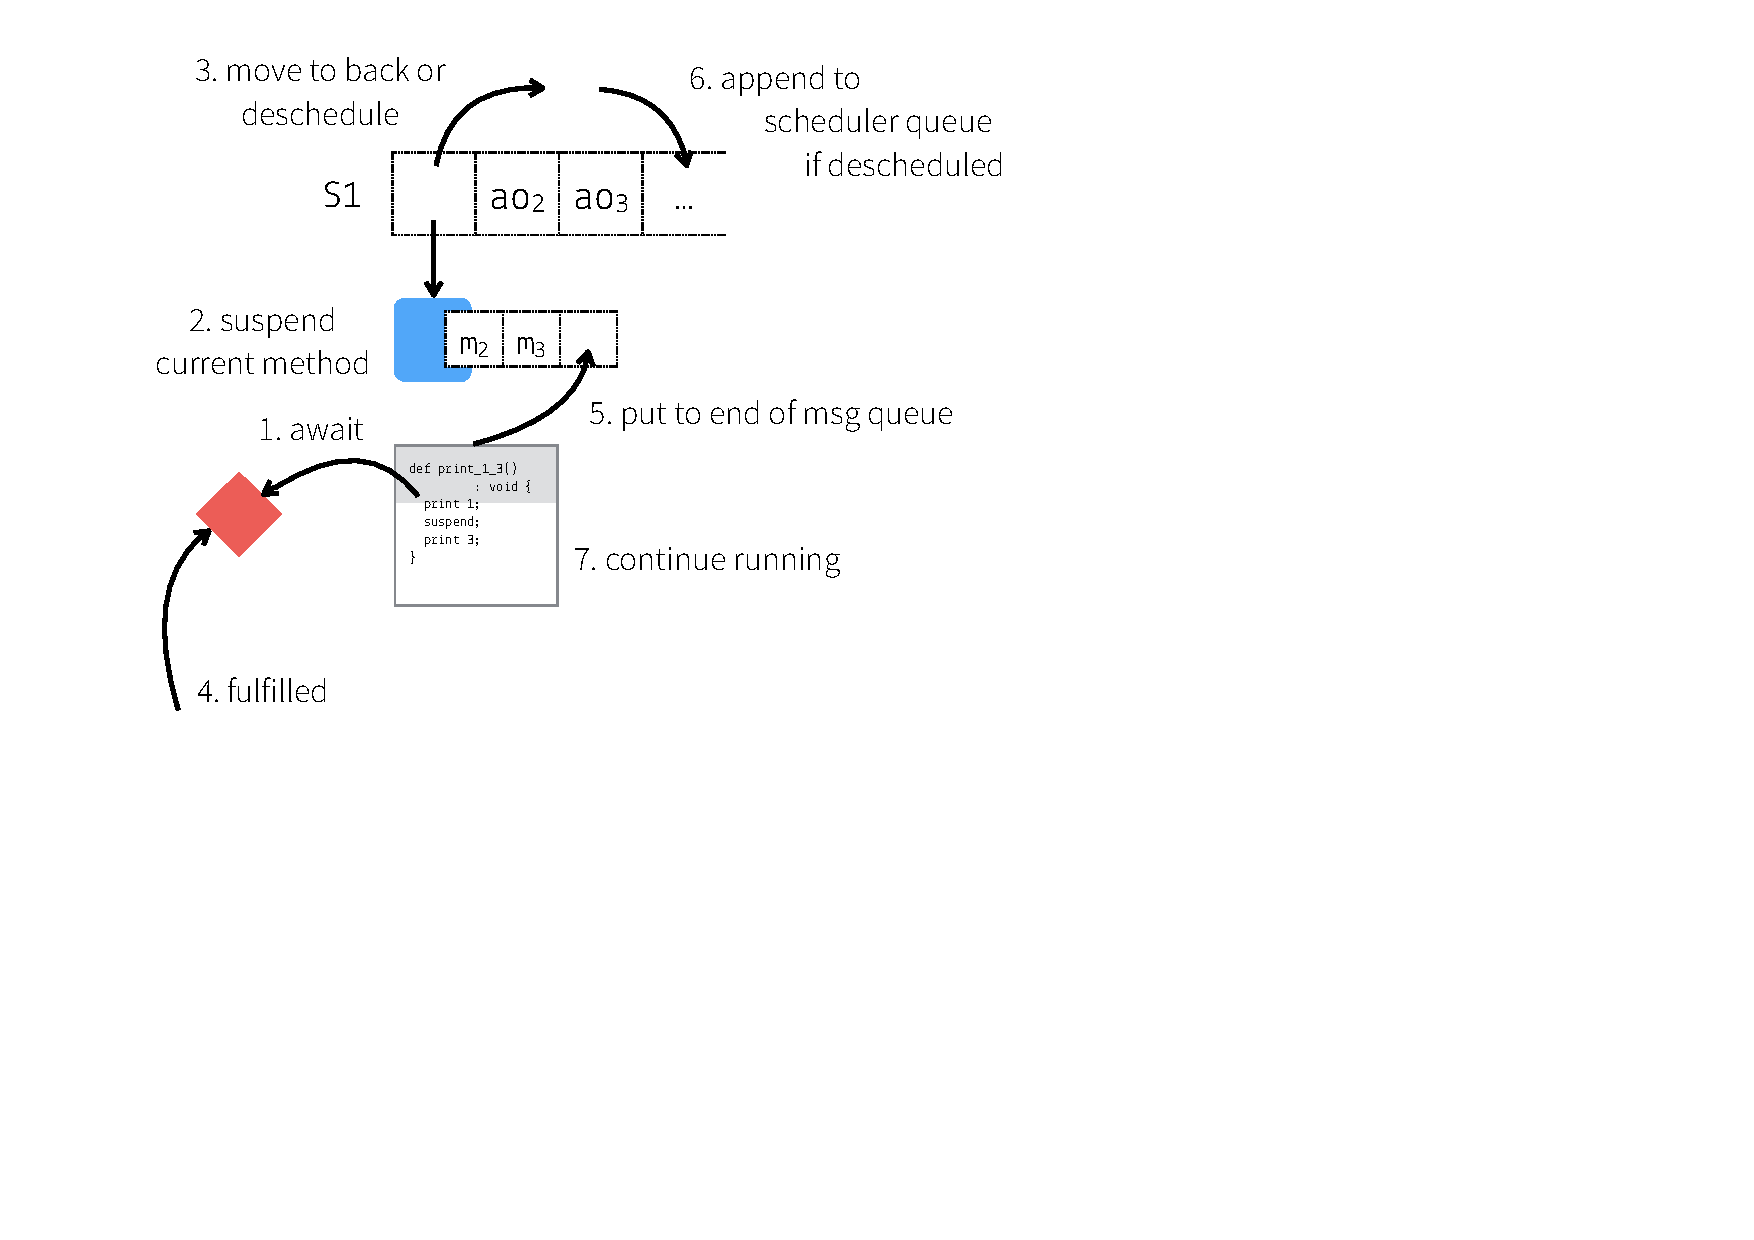
\includegraphics[scale=.42]{pictures/enc-await-unfulfilled}
	\caption{(Left) An Encore program executing a \ec{get} on an
          unresolved future. This causes the currently executing
          active object to be unscheduled, only to be rescheduled
          after the future has been resolved. Once the object gets to
          the head of the scheduling queue after this point, the
          \ec{get} operation returns and the program continues from
          this point.  with non-empty message queues. (Right) An
          Encore program executing an \ec{await} on an unresolved
          future. In contrast to \ec{get}, the active object is only
          unscheduled if it does not have any messages in its message
          queue, and once the future is resolved, the resuming method
          is placed at the end of the active object's queue.}
	\label{fig:enc-get-await}
\end{figure}
%As described in Section~\ref{sec:encore}, when the active object processes a message
%and a synchronization construct is involved, the running method may be paused
%until a future is fulfilled and resumed afterwards.

Unlike the ProActive backend for ABS that relies on creating new
threads, Encore opts for handling stacks, which can be attached to
\emph{encore threads}. Based on this idea, the current stack is put
aside and a new stack is given to the \emph{encore thread}, so that it
can continue running some other or the same active object using the
new stack.  To make this process more efficient, Encore has a stack
pool that allows reusing unused stacks.  Upon resolution of the
awaited future, the \emph{encore thread} can continue processing the
suspended execution and, when it has finished, the stack is collected
and returned to the stack pool for future reuse.

%could be paused in the middle, and be resumed when the request service is scheduled
%again. All information living on the stack must be preserved for message
%processing continuation. Currently, Encore runtime fetches a free stack page
%from the stack pool to process next active object, this new stack page is used
%until next pause happen. When message processing finished, the stack page is
%collected and returned to the stack pool for future reuse.

\paragraph{Data sharing and object referencing}

Active and passive objects in Encore are shared by reference, as
opposed to ProActive which performs deep copying of the object
(Section~\ref{sec:implem-proactive}).  In practice this means that
sharing large objects in Encore poses no performance issues.
%
On the other hand, care must be taken when sharing passive objects, as
these are mutable by default and, without the use of a proper
capability type, could introduce data races.
%
Active objects are not subject to this problem, they run in an
\emph{encore thread} which provides its own thread of control.
%
In terms of the capability system, immutable passive objects are
immune to this problem for obvious reasons.
%
Following this line, a locked mutable passive object provides locking
guarantees on the object, which prevents data races.
%
In a slightly more advanced usage scenario, we might share part of the
mutable passive object so that multiple active objects could work on
different parts of the same passive object, concurrently. This would
be safe as well.
%
However, the capability system is work in progress and not yet
available in the compiler.

\paragraph{Error handling}

Currently, Encore offers limited support for exception handling. Errors can be expressed
using option types, where \verb|Nothing| could represent the error, and programmers can
pattern match on it.

\paragraph{Garbage collection}

Encore borrows the garbage collector from PonyRT with the necessary
extension to accommodate future values. Garbage collection consists of
two parts, collecting active objects, which is covered by Clebsch and
Drossopoulou~\citeyear{DBLP:conf/oopsla/ClebschD13}, and collecting
passive objects.

\subsection{Erlang Backend for Rebeca}

Execution of Rebeca models is performed by translating Rebeca models to Erlang code.
% \cite{DBLP:journals/scp/ReynissonSACJIS14}.
Erlang is a dynamically-typed general-purpose programming language for
distributed, real-time and fault-tolerant applications with an
actor-based concurrency model. Having the same concurrency model,
translating Rebeca models to Erlang is realized by a direct mapping of
language constructs \cite{DBLP:journals/scp/ReynissonSACJIS14}.

\paragraph{Thread creation and scheduling}

Actors, as the only concurrent elements of Rebeca models, are mapped to processes in
Erlang, concurrently executing elements that are very much lighter than OS-level threads
(more than 100,000 of them can be run on a single computer) \cite{Erlang-book}. The
programming facilities of Erlang for developing concurrent applications (i.e., spawn,
``!'', and receive) allow processes to create new processes and to communicate through
asynchronous message passing. These capabilities are used to translate Rebeca models to
Erlang code without the need for modification. The generated processes are scheduled
by the default scheduler of Erlang, the so-called reduction-based scheduler.
%To model the actors scheduler of Rebeca, reduction-based scheduler of Erlang is used. Using reduction-based scheduler, an Erlang process is allowed to execute for a time slice of approximately 2000 reductions before a context switch occurs. A reduction corresponds to the execution of one of the Erlang's built-in functions.% So, a single reduction is not a constant value.

\paragraph{Data sharing and object referencing}

Reserving a dedicated memory space for each process in Erlang avoids the need for shared
objects among processes. When object communication happens, the sent message and its parameters must be
stored in the message bag of the receiver actor which is located in its dedicated memory
space. %So, a copy of the parameters is stored in the receiver's memory space. %This
%%mechanism is called copying message passing of Erlang.
%\LUDO{the end is not clear to me}
%Although, passing reference of actors using this mechanism does not result in sending
%the deep-copy of actors and only reference to actors are copied and are sent.
References to actors are permitted for the purpose of sending messages
(although not for sharing data among actors).

\paragraph{Error handling}

In the current version of Rebeca, there is no mechanism for exception handling; the
programmer must rely on traditional messages to deal with errors. %So, modelers have to
%handle exceptions manually. In other words, exception handling is not a special case in
%Rebeca models and they must be implemented the same as ordinary parts of message servers
%of actors.
%Currently, Rebeca doesn't have support for exception handling.
%Codes for handing errors must be implemented the same as ordinary parts of message
%servers of actors.


\paragraph{Garbage collection}

Rebeca borrows the default garbage collector of Erlang without any modification, which
runs one garbage collector for each process,  handling garbage collection internally within
each actor. %It uses general garbage collection
%algorithm (dividing memory to young and old generations) for each process.
%\LUDO{I do not understand the last two sentences}
%This way, as each Rebeca actor is mapped to one Erlang process, we can say that per
%actor garbage collection takes place in translated codes. %In addition, the intra
%%process
%%garbage collection only analyses large processes (i.e., processes which consumes more
%%than 20K of memory). So,
%In memory pressure, all of the Rebeca actors are analyzed to this aim as they are
%long-lived large processes.

% Einar
\section{Discussion}\label{sec-discussion}

\subsection{Design Trade-Offs in Active Object Languages}
\label{sec:design-trade-offs}

The four languages reviewed here start out from the same programming
model, the active object paradigm, but address different challenges,
motivated in the context of different design goals. We review the
different design trade-offs.

\noindent
{\small \sf
\begin{tabular}[t]{|@{\,\,}p{15mm}@{\,\,}|@{\,\,}p{27mm}@{\,\,}|@{\,\,}p{29mm}@{\,\,}|@{\,\,}p{29mm}@{\,\,}|@{\,\,}p{28.5mm}@{\,\,}|}
\hline
& \textbf{Rebeca} & \textbf{ABS} & \textbf{ASP/ProActive} & \textbf{Encore}\\\hline
\textbf{Objective}&$\bullet$ Actor-based  modeling  language\newline $\bullet$
           Simple compu\-tation and communication model\newline
           $\bullet$ No dynamic\newline object creation&$\bullet$ Active object\newline
                                                 modeling
                                                 language
                                                 \newline $\bullet$
                                                 COGs \newline
                                                 $\bullet$ Combines
                                                 functional and
                                                 imperative features
                                                 \newline $\bullet$
                                                 Advanced
                                                 communication
                                                 model&$\bullet$  Active object\newline
                                                        programming\newline
                                                        language\newline
                                                 $\bullet$ Multiactive objects \newline
                                                                                $\bullet$
  Designed for\newline  distribution&$\bullet$  Active object\newline
                                                        programming\newline
                                                        language
                                                                                \newline
                                                                                $\bullet$
  Designed for\newline  scalability\\\hline
\textbf{Degree of\newline synchro\-nization}&$\bullet$ Asynchronous \newline message
                           passing\newline $\bullet$ No
                           synchro-\newline nization\newline
                                                          $\bullet$
                           Single-threaded run-to-completion of
                           requests per\newline  actor&$\bullet$ Asynchronous \newline
                                            method calls with \newline first-class
                                            futures \newline
                                            $\bullet$ Advanced\newline
                                            synchronization\newline
                                            $\bullet$ Cooperative
                                            sche\-duling interleaves
                                               requests per COG &$\bullet$
                                                              Implicit
                                                              futures
                                                              \newline
                                                              $\bullet$
                                                              Wait by
                                                              necessity
                                                          synchronization\newline
                                                          $\bullet$
                                                              Multiactive
                                                          objects
                                                              allow
                                                              parallel
                                                          treat-
                                                                  \newline ment of
                                                          requests&$\bullet$
  ABS-like cooperative scheduling \newline $\bullet$ Future chaining
\newline $\bullet$ Multiactive\newline
                                                          objects
                                                                    using
                                                                    parallel
                                                                    combinators
                                                                    for\newline
                                                                    data parallelism
  \\\hline
\textbf{Degree of\newline transpa\-rency}&$\bullet$ Hides\newline
                                           asynchronous message
                        passing\newline $\bullet$ Hides\newline scheduling and\newline message queues&$\bullet$ Hides object\newline  representation,
                         scheduling, and\newline  message queues
                  \newline $\bullet$ Exposes
                         futures\newline and
                         release points&$\bullet$ Hides futures and\newline distribution
                                         \newline $\bullet$
                                         Exposes parallel\newline treatment of\newline
                                 requests&$\bullet$ Hides scheduling
                                           and low-level\newline
                                           parallelism \newline $\bullet$ Exposes
                         futures,
                         release  points, and parallel data flow\\\hline
\textbf{Degree of\newline data sharing}&$\bullet$ No shared values\newline $\bullet$
                        All arguments\newline  passed by copy,\newline  even actor
                        refer-\newline ences&$\bullet$ No
                                    shared values \newline $\bullet$ Objects
                                 passed by\newline reference\newline
                                              $\bullet$ Functional
                                              values\newline passed
                                    by  copy \newline $\bullet$
                                    Private fields&$\bullet$ No
                                                        shared
                                                        values\newline
                                                          $\bullet$ Active
                                                        objects pas\-sed
                                                          by
                                                        reference\newline
                                                        $\bullet$ Passive
                                                        objects\newline passed
                                                          by
                                                        copy&$\bullet$
                                                              Active
                                                              objects
                                                              pas\-sed
                                                              by
                                                              reference\newline
                                                              $\bullet$
  Capability types\newline control data sharing\newline for passive objects\\\hline
\textbf{Implemen\-tation and\newline tooling support}&$\bullet$ Model checking&$\bullet$
                                                             Simulation\newline
                                                             $\bullet$ Wide
                                                   range of\newline  analysis
                                                   tools\newline $\bullet$  Code generation&
                                                          $\bullet$
                                                        Implemented as
                                                          a\newline  Java
                                                                                             library\newline
                                                                                             $\bullet$
                                                          Supports
                                                                                             distri-\newline buted
                                                                                             architectures&$\bullet$
  Runtime system\newline  written in C\newline $\bullet$ Supports multi-\newline core architectures\\\hline
\end{tabular}}


\paragraph{Degree of synchronisation}
The degree of synchronisation is  a design choice that is central to the
design of parallel programming languages. The original actor model has a  semantics
where  communications are purely asynchronous and no strict
synchronisation exists. This resembles the principles of Rebeca. However in Rebeca, it
revealed useful to ensure FIFO message communication to provide some guarantees on
ordering of operations. From a global perspective, synchronisation hinders efficiency and
parallelism, but makes programming easier, and sometimes more efficient. The other
programming languages we presented allow the programs to synchronize on the result of a
method invocation through the use of futures. However, different synchronisation patterns
exist on futures: from strict synchronisation like the \texttt{get} operator if ABS to
asynchronous reaction to future fulfilment enabled by future chaining
in Encore. Two synchronisation patterns on futures presented in this article feature an
interesting compromise: the \texttt{await} operation of ABS and Encore enables
cooperative
multi-threading and let the program serve another request while the future is
awaited; and the wait-by-necessity synchronisation of ProActive that automatically waits
upon the
availability of useful data, wait-by-necessity allows the program to pass futures around
and never worry
about imbricated futures.
Different \emph{communication paradigms} also have been investigated in the proposed
languages,
the extreme cases being the causally ordered communications ensured by ASP which makes
programming easier because of the ordering guaranteed to the programmer, and the full
asynchronous communication as described in the semantics of ABS which allows more
parallelism and better overlapping between communication and computation. However it is
interesting to note that even with an asynchronous communication as the default
semantics, many implementations of ABS ensure FIFO ordering of messages.

\paragraph{Degree of transparency}
The degree of transparency is very much related to the syncronisation primitives.
In
practice there is for the moment mostly two extreme approaches: either everything is
very explicit and the user syntactically differentiates asynchronous invocations from
synchronous ones (e.g., $o!m()$ vs. $o.m()$ in ABS) or everything is hidden to the
programmer who programs active objects like if they were sequential objects and where
synchronisation on method results is hidden to the programmer. In Rebeca, explicitness is
even stronger as the remotely invokable methods are declared by a specific syntax and do
not
return a result.

\paragraph{Data sharing and data access}
By principle and according to the Actor programming paradigm, active objects do not share
memory; however, at least some objects can be accessed by any other object.
Data sharing plays especially an important role in relation to the implementation.
Indeed, ASP that was designed in close relation to Java RMI because of the implementation
of the ProActive library, features a non-uniform active object model where some objects
are
active and can be invoked from anywhere and others are transmitted by copy. From another
point of view, ABS was designed as a specification language where each object can be
invoked by any other object; the first implementations of ABS did not support
distribution, and the distributed implementations have to provide a hierarchical way of
addressing objects in order to scale. Encore has a particular role here as it
is  focused on efficient local parallelism where it is possible to have efficient
addressing of many objects; this allows an implementation of passive objects
where no data is copied and a better efficiency is provided.

It is interesting to notice that both ABS and Encore allow the programmer to depart from
the
pure actor model by providing local multi-threading to an actor,
either inside the treatment of a request (the parallel combinators of
Encore) or by running several requests in parallel (the multi-threaded
active objects of ASP). In each case, the extension of the language is
provided in such a way that it relies on the same programming
abstractions as classical active objects and for this reason, it is
still very easy to write safe and efficient programs. In both cases, multi-threading
allows the programs to gain efficiency by better using local concurrency, it also allows
the programmer to express some parallelism patterns that are difficult to write with
classical active objects. It is important to notice that, even if the strict
mono-threading policy of actors can be broken in those language, the programming language
still strictly guarantees that no data-race can exist between two different actors.


\paragraph{Formal semantics}
It is noteworthy that all four languages are equipped with a \emph{formal
semantics}, which is the basis for unambiguous implementations and for
far reaching tool support in terms of static analysis tools, test
generators, optimizers, etc. For several of the languages discussed
here meta properties of the formal semantics were proven, such as type
safety or data race-freedom.

\paragraph{Tooling and execution support}
Both Rebeca and ABS started with a strong focus on tool-based formal
analysis and verification, but recently added fairly efficient
implementations. For this both languages rely on cross translation.
On the other hand, ProActive and Encore focused on efficient
implementation on distributed and many-core computer architectures,
respectively. Both come with ``native'' implementations based on
extensions of existing frameworks.

 Rebeca is probably the language that features the most variety in the
variants of the languages that can be checked and the different language semantics that
can be verified. ABS on the contrary comes with very different analyses based on the same
semantics. Both languages show the advantage of adopting an active object programming
paradigm compared to standard models of distribution and concurrency concerning
 verifiability of programs. On the other side, ASP and Encore mostly focused on the
execution support tools. While powerful verification tools also exist for those language,
significant efforts have been made on the efficiency of the local parallelism in Encore,
and on the support for effective large-scale distribution in ProActive. ProActive
programs targets HPC applications: setting up the program
environment is complex, but the distributed execution is efficient on
the whole; a few active objects co-exist in an application. The Java 8
backend for ABS provides light threads and enables instantiation of
many active objects on the same machine. It also permits active
objects to achieve faster communication than in ProActive. At a finer
granularity, Encore provides optimized constructs that allow safe and
efficient programming at a low level of abstraction.

Concerning implementation, the different execution environment provided in this paper
cover a wide range of the possible ways to implement an active object language.
Indeed, a language can be implemented from scratch with a whole compiler tool-chain	but
to offer a more efficient runtime support and to minimise the implementation effort all
the languages presented here rely on an existing widely adopted language. Encore is
probably the closest to a full implementation of a language and runtime support, as it
compiles to C and requires a dedicated runtime environment. It is also probably the most
efficient local implementation of active objects. Rebeca and ABS mostly rely on
compilation to high-level languages, sometimes augmented with a dedicated API. ProActive
takes a different approach and is implemented as a library of an existing language,
allowing the programmer to use almost all the functionalities of the host language,
modulo a few natural restrictions. Finally, this article also presented a ProActive
backend for ABS, illustrating the possibility to cross-translate an active object
language into another one.


\subsection{Other High-level Concurrent Languages}
\label{sec:other-high-level}

There are several other programming languages that introduce
high-level abstractions for concurrent programming that deviate from
the active object approach.  JAC~\cite{ref:jac} stands for Java
Annotations for Concurrency. It provides Java annotations that allow
the programmer to specify the kind of parallelism that can occur
inside a Java object from a relatively high-level perspective. It is
possible to encode versions of actors in JAC.
%
The concurrency model of
AmbientTalk~\cite{Dedecker:2006:APA:2171327.2171349} is based on the E
Programming Language~\cite{Miller05concurrencyamong} which implements
a communicating event-loop actor model with fully asynchronous futures
(called promises): calls on futures trigger an asynchronous invocation
that will be executed when the future is available and objects are
passed by eventual reference between actors rather than by copy. This
facilitates the creation of many small, object-level interfaces (each
eventual reference acts as a new entry point to the actor), rather
than a single large actor-level interface. AmbientTalk adds new
primitives to handle disconnecting and reconnecting nodes in a network
to support ambient-oriented programming.
%
In Panini \cite{LinRajan13} concurrent behavior is specified by
composing modules (called ``capsules'') that by themselves behave
sequentially. The granularity of concurrency is more coarse-grained
than in active object languages and there are no explicit
synchronization statements.

Akka~\cite{haller2009scala,AkkaBook} is a scalable library for
implementing actors on top of Java and Scala.  Akka Typed Actors is an
implementation of the Active Objects pattern.
%
%\subsubsection*{Active object languages with industrial support: Akka and Orleans}
%Based on the overview presented in this paper, it seems interesting
% to focus on two modern industrial languages based on the active
% object paradigm. We review the two frameworks Akka and Orleans, from
% the point of view of the languages presented here. The success of
% these two frameworks show the practical usability of the active
% object programming model and its adequacy to program large scale
% industrial software.
%
%\paragraph{Akka}
%Akka~\cite{haller2009scala,AkkaBook} is an actor-based message-driven
% runtime for managing concurrency, elasticity and resilience on the
% Java Virtual Machine with support for both Java and Scala.  It is an
% open core development platform for Akka distributed systems runtime,
% play web framework, lagom microservices framework, and Apache Spark
% in-memory compute engine for Java and Scala.
All interactions of actors in Akka use only message passing and all
communication is asynchronous.
% Programmers need to provide a pattern match for all messages that it
% can accept.  To be able to handle unknown messages, a default case
% is required.
Actors interact identically, regardless whether they are on the same
or separate hosts, communicating directly or through routing
facilities, running on a few threads or many threads, etc. Such
details may be altered at deployment time through a configuration
mechanism, allowing a program to make use of more (powerful) servers
without modification.  Akka is ideally suited for hybrid cloud
architectures and the elastic scaling of cloud platforms. In one
experiment it only took four minutes to start a 1000-node Akka cluster
on Google Compute Engine (GCE), including the time to start the GCE
instances.
% In Akka, actors form a tree with actors being parents to the actors
% they've created. As a parent, the actor is responsible for handling
% its children's failures (supervision), forming a chain of
% responsibility.  Accordingly, Besides, Akka supports error handling.
% It embraces the reality of unplanned errors and adopts a pragmatic
% ``Let It Crash'' philosophy using supervision and self-healing to
% ensure impacted components are reset to a stable state and restarted
% upon failure.

%\paragraph{Orleans}
Orleans~\cite{BykovGKLPT11,BernsteinB16} is an actor framework
developed at Microsoft research and used in several Microsoft
products, including online games relying on a cloud
infrastructure. Its strength is the runtime support for the creation,
execution, and state management of actors.
% From a language point of view, Orleans does not provide a publicly
% available formal semantics nor an exhaustive and precise description
% of the behaviour of the programming primitives.
Orleans relies on a non-uniform active object model with copies of
transmitted passive objects, like ASP. The semantics of futures is
based on continuations and relies on an \ec{await} statement similar
to that of ABS and Encore, however, there is no primitive for
cooperative scheduling. Consequently, the programmer has to take care
of possible modifications of the object state between the \ec{await}
and the future access. This semantics for future access is similar to
the way futures are handled in general in Akka.
%
There is extensive runtime support in the Orleans
framework. Importantly, it supports the efficient creation,
activation, and deactivation of active objects governed by the
requirements of an application. This is why Orleans is called a
\emph{virtual actor model}.  Orleans also focuses on efficient
execution of active objects, including optimized serialization for
inter-actor data transmission. Both, object management and data
transmission, scale in terms of distribution and in terms of the
number of active objects that can interact within a single
application.
% The Orleans runtime also supports the application in the management
% of resources, storage, errors, failures, and recovery.

\section{Lessons Learned and Conclusion}\label{sec-conclusion}

%\JS{There is an increased parallelism in new active object programming languages.
%
%}

%\KIKO{

With the advent of many-core computers and large-scale cloud
computing, the active object paradigm evolved out of actor-based
concurrency as one of the most promising candidates to model
asynchronously parallel and distributed computations in a safe manner.
%
We retraced the unfolding of the active object paradigm during the
past fifteen years by focusing on four representative active object
languages. We are convinced that active object concepts will
eventually make their way into mainstream programming languages (the
adoption of an actor system in Scala is a first indicator). Therefore,
it is essential to understand the trade-offs involved in their design
and implementation.



In Section~\ref{sec-implementation} it was shown how the semantics of
each language influenced its implementation, how different design
decisions create new challenges, how these have been addressed, and
which limitations remain.  One important dimension along which the
languages can be distinguished is how they handle efficient data
sharing, and how each language finds a balance between copying and
safe shared memory.



We hope that the trade-offs and options discussed in this survey can
serve as a future reference for designers and implementors of
programming languages that make use of the active object paradigm.



%\section{Introduction}\label{Introduction}
%
\section{Generalities about actors and active objects}
\emph{We should probably start by  a section giving the common principles of actor and 
active object languages, giving also the vocabulary}

The active object model is  derived from the Actors
model \cite{DBLP:conf/birthday/AghaT04,agha97foundation,Agha86-book}. Actors and active objects share
a lot of concerns and advantages. A great part of the mechanisms
designed for one programming paradigm can be applied, almost
straightforwardly, to the other.


The principle of active objects is very simple: An object is said to be
active if it can be deployed on a remote machine. As a consequence,
every call to such an object will be a remote method invocation; we
call such an invocation a \emph{request}. An active object is thus an
object that treats the requests it receives, it is an object together
with a thread.

To decouple the invocation object from the invoked object, contrarily
to a classical remote invocation, the invoker is not blocked waiting
for the result instead a future object is created and represents the
result of the remote invocation.

Futures, first introduced in Multilisp \cite{Halstead85} and ABCL/f~\cite{ABCL1994}
are used as constructs for concurrency and data
flow synchronisation. Futures are language constructs that improve
concurrency in a natural and transparent way. A future represents a
result that has not been computed yet. When the result is available it
can be retrieved (automatically or manually), we then say that the
future is \emph{resolved}.
Frameworks that make use
of explicit constructs for creating futures include
Multilisp~\cite{Halstead85}, $\lambda$-calculus \cite{jlambda-fut06}, Creol
\cite{Elinar2006}, SafeFuture API \cite{SafeFutures05}, and ABCL/f
\cite{ABCL1994}. In contrast, futures are created implicitly in
frameworks like  ASP \cite{CHS:POPL04}, \cite{CHS-IC2008},
\cite{CH-book},
AmbientTalk~\cite{DedeckerCMDM-ecoop06},
ProActive~\cite{CDD:CMST06}.  Usually, in those object-oriented languages,
implicit creation corresponds to asynchronous method invocation. A key
benefit of the implicit creation is that no distinction is made
between synchronous and asynchronous operations in the program.
This way, when a method invocation is local, usual method invocation
is performed, whether when the accessed object is remote, a future is
immediately obtained.

Additionally, the futures can be accessed explicitly or implicitly. In
case of explicit access, operations like \emph{claim} and \emph{get},
\emph{touch} are used to access the future \cite{Elinar2006,ABCL1994}.
For implicit access, operations that need the real value of an object
(\emph{blocking} operations) automatically trigger synchronisation
with the future update operation. We say that futures are \emph{first
	class} if future references can be transmitted between remote
entities without requiring the future to be resolved.



\section{Criteria for comparison}
\emph{Here we suggest to summarise the points of comparison between different active 
object languages}


The principle of active objects is to associate a thread to an object, or to a set of
objects. We call \emph{activity} this notion: a thread and the objects
managed by this thread.  Two objects in different activities 
communicate by remote method invocation: when an object invokes a
method on an object in another activity, this creates a
\emph{request}; the invoker continues its execution while the invoked
object will serve the request in an asynchronous manner. Requests wait for execution in a \emph{request queue}. Like in any
object-oriented language, method invocations can return results. In
order to allow the invoker to continue its execution, a placeholder
for the expected result must be created. \emph{Futures} play this
role: a future is an empty object that will later be filled by the
result of a request. We say that a future is \emph{resolved} when its
value is known.
Overall, the active object paradigm makes programming of distributed
applications more natural, especially when applications are made of
computational entities that may have a state like objects, and that
execute in a decoupled manner because they are distributed.
While all active object models rely on the previously introduced notions, their
detailed characteristics vary in practice, which we present below:

\subsubsection{How are objects associated to activities?}\label{sec:activity}
We distinguish three different ways to map objects to threads/activities: 
\begin{itemize}
	\item \textit{Uniform Object Model.}  All objects are active objects
	with their own request queue and their own private execution thread.
	In consequence, all communications between objects occur by posting
	a request. This model is simple to formalise but its implementation
	is more difficult as it must rely on the creation of logical thread
	to allow scalability.
	\item \textit{Non Uniform Object Model.}  Some of the objects are not
	active, in which case they are only accessible by a single active
	object, they are part of its state. 
	An activity contains one active and several passive objects. Non-uniform active object models
	are much more efficient as they require less communications and
	less concurrent threads than models where each object would be
	active. Reducing the number of activities also reduces the number of
	references that are globally accessible in the system, and thus enables the
	instantiation of a large number of objects.
	\item \textit{Object Group Model.}
	In this model, an activity is made of a set of objects sharing a
	request queue and an execution thread, but all
	objects can be invoked from another activity. This
	approach improves scalability as it reduces the number of threads, but
	it is still difficult to create a lot of objects as all of them must
	be registered so that they are accessible from any other activity.
\end{itemize}

\subsubsection{How are requests scheduled?}
We distinguish three  threading models in active object languages.
\begin{description}
	\item \textit{Single-threaded.} 
	Within an active object, requests are executed sequentially without
	interleaving possibilities. 
	\item \textit{Cooperative scheduling.}
	A running request can explicitly release the execution thread to let
	another request run. Requests are not processed in parallel but they
	might interleave. Data-races are avoided.
	\item \textit{Multi-threaded.}
	Within an active object, requests are executed in parallel using
	different threads, without pausing nor yielding.
	Some data-races inside the activity is possible. This is
	called a \emph{multiactive object} model.
\end{description}

\subsubsection{Is the programmer aware of distributed aspects?}
Some active object languages use a specific syntax for asynchronous
method calls: a different operator is used to distinguish them from
synchronous method calls. This makes the programmer aware of the
places where futures are created. Generally, when asynchronous
invocation is explicit, there exists a special type for future objects.
Additionally, the futures, when they are statically identified, can be
accessed explicitly or implicitly. In case of explicit access,
operations like \emph{claim}, \emph{get} and \emph{touch} are used to
access the future. This is particularly convenient for releasing the
current thread if a future is not available in case of cooperative
scheduling (\emph{await} statement). For implicit access, operations that need the real
value of an object (\emph{blocking} operations) automatically trigger
synchronisation with the future update operation.
Implicit future creation allows transparency of distributed aspects:
there is almost no difference between a distributed program and usual
objects, whereas explicit manipulation of futures allows the
programmer to better control its execution, but requires from him a
better expertise. We say that futures
are \emph{first class} if future references can be transmitted between
remote entities without requiring the future to be resolved.





\section{Active object and Actor languages}\label{sec:overview}
\emph{Here we suggest to have a list of active object languages referring to the 
preceding classification}

Several programming languages or models rely on some form of active
objects, we review the main ones below. Especially focusing on
languages which have a formalised semantics. But before focusing on
active objects, let us first review the main works on formalisation of
futures in the context of functional languages.
Indeed, Futures
were first introduced in Multilisp \cite{Halstead85}, and thus lead to
a lot of work on their formalisation in the context of 
functional languages. We will then review main active object languages
and finish by a couple of languages that are not pure active objects
but also strongly relate the notions of distribution and concurrency to
the notion of objects.



\subsection{Futures in functional languages}
To our knowledge, the first work on formalisation by semantic rules of
Futures appeared in \cite{FlanaganFelleisen99,FlanaganFelleisen1995} and was intended at
program optimisation. This work focuses on the futures  of MultiLisp,
that are explicitly created. The authors ``compile'' a program with
futures into a low-level program that does explicit touch operations
for resolving the future, and then optimise the number of necessary touch operations.

In a similar vein,
$\lambda(fut)$ is a concurrent lambda calculus with futures.
It features non determinism primitives (cells and handles). In
\cite{jlambda-fut06}, the authors define a semantics for this calculus,
and two type systems. They use
futures with explicit creation point in the context of $\lambda$-calculus; much in
the same spirit as in Multilisp. Alice~\cite{Niehren:Sabel:Schmidt-Schauss:Schwinghammer:06} is an
ML-like language that can be considered as an implementation of
$\lambda(fut)$.



\subsection{Asynchronous Sequential Processes}
The ASP calculus we have defined~\cite{CH-book} is a distributed active object calculus with futures;  the
ProActive library \cite{CDD:CMST06} can be considered as its reference
implementation.  The ASP calculus formalises the
following characteristics of active objects:
\begin{itemize}
	\item \emph{asynchronous communications}, by a request-reply mechanism;
	\item \emph{futures}; in ASP, futures are transparent
	objects: their creation and access is implicit, futures are also
	\emph{first-class}: they can replace
	transparently any other objects and can be communicated as 
	result or parameter of remote method invocations;
	\item \emph{sequential execution} within each process, each object
	is manipulated by a single thread;
	\item \emph{imperative objects}, i.e. each object has a state and
	there is an operation for updating it.
\end{itemize}

ASP's active objects are quite similar to actors and ensure the
absence of sharing: objects live in disjoint activities. An activity
is a set of objects managed by a unique process and a unique
active object.  Active objects are accessible through global/distant
references.  They communicate through asynchronous method calls with
futures. 
ASP is a non-uniform active object model: some of the objects are
not active, in which case they are only accessible by a single active
object, they are part of its state. Non-uniform active object models
are much more efficient as they require much less communications and
much less concurrent threads than models where each object would be
active.

Our main result consists in a confluence property and its
application to the identification of a set of programs behaving
deterministically.  This property can be summarised as follows:
\begin{itemize}
	\item 
	Future updates can occur at any time without any consequence on the
	result of the computation,
	\item Execution is only characterised by the order of requests, and
	even more precisely by the order of request senders: To characterise
	uniquely an execution,
	it is sufficient to consider, for each activity, the ordered list
	of identifiers of the activities that have sent a request to this activity.
	\item Consequently, programs communicating over trees are deterministic.
\end{itemize}


The code snippet shown in Figure~\ref{fig:pasniplet} gives a typical
example of a simple ProActive piece of code. It
creates a new active object of type \code{A} on the JVM identified
by \code{Node1}. All calls to that remote object will be
asynchronous, and the access to the result might be subject to \emph{wait-by-necessity}.
% \begin{small}
\begin{figure*}[t]
	\begin{lstlisting}[frame=single]
	A a = (A) ProActive.newActive("A", params, Node1); // active object creation
	v = a.bar (...);   // Asynchronous call, no wait, v gets a future
	o.gee (v);         // No wait, even if o is a remote active object and v is still awaited
	...
	v.f (...);        // Wait-by-necessity: wait until v gets its value
	\end{lstlisting}  % \end{verbatim}
	\caption{Typical ProActive code}
	\label{fig:pasniplet}
\end{figure*}% \end{small}

\smallskip

The main advantage of ASP is that most code can be written without
caring about distribution and concurrency.  Futures are automatically
and transparently created upon method invocation on an active object.
Synchronisation is due to wait-by-necessity that occurs
upon access to a future that has not been resolved yet.
This synchronisation is performed transparently, i.e. 
there is no  construct for explicitly waiting the result of
a request. Wait-by-necessity is always
performed at the last moment, i.e. when a value is really needed.
Futures are also transparently sent between activities. This
way simple programs can be written extremely easily and rapidly.


Recent works tend to introduce local concurrency either at the actor
level
\cite{Scholliers:2014:PAM:2563745.2564410,ref:spec-actors} or at the
active object level, in particular with multiactive objects
\cite{ref:mao}.
Multiactive objects avoid deadlocks that are likely to arise
%when doing reentrant calls 
with mono-threaded active objects, and take
advantage of multi-core architectures.  
%The principle of multiactive objects is to execute
%multiple requests of an active object in parallel, while controlling
%the concurrency.
%The multiactive object model has been implemented as an extension of ProActive. This 
%extension comes as a small metalanguage to allow 
In practice, a programmer declares which requests of an active object can safely be
executed in parallel, namely which requests are \emph{compatible}. An implementation of 
multiactive objects is available in the latest version of ProActive; 
%The
%metalanguage to do that in ProActive 
it is based on the Java annotation
mechanism:
% A programmer can use these annotations on top of a class so that all objects of this 
%class are automatically multiactive objects when instanciated with the \code{newActive} 
%ProActive primitive\footnote{if there is no annotation, then objects crerated with the 
%\code{newActive} primitive remain basic active objects}. 
%Request compatibility can be specified following three steps:
%\begin{itemize}
%\item A programmer first uses the \code{@Group} annotation on top of a class to define a 
%group of requests. A group is meant to gather requests that have the same concerns 
%and/or 
%the same compatibility requirements. 
%\item Then, a programmer uses the \code{@MemberOf} annotation on top of a method 
%definition to make this method belong to a particular group (previously defined).
%\item Finally a programmer uses the \code{@Compatible} annotation to specify which group 
%is compatible with which other group, so, in extension, to specify which requests can be 
%run in parallel safely. 
%\end{itemize}
%Below is an example of an annotated
%class \code{MyClass}:
%\ttfamily\scriptsize
\setlength\abovecaptionskip{0.25mm}
\lstset{
	morekeywords={@DefineGroups,@Compatible,@DefineRules,@Group,@MemberOf},
} 
\begin{lstlisting}
@Group(name="group1", selfCompatible=true)
@Group(name="group2", selfCompatible=false)
@Compatible({"group1", "group2"})
public class MyClass {
...
@MemberOf("group1")   public ... method1(...) { ... }
@MemberOf("group2")   public ... method2(...) { ... }
}
\end{lstlisting}
In this example, groups of requests are defined with \code{@Group} and filled with
\code{@MemberOf}. Group compatibilities are specified with
\code{@Compatible}. Parameter \code{selfCompatible} defines
whether two different requests of the same group are allowed to run in
parallel.  Upon execution, a ready request is executed if it is
compatible with requests that are executing and with older
requests in the queue to avoid starvation.  


It is also possible to set a limit on the number of threads running in
parallel~\cite{henrio:hal-00916293}.  The limit can be applied in two ways: a hard limit
restrains the overall number of threads whereas a soft limit only counts threads that are
not in wait-by-necessity.  Additionally, threads can be limited per group.

Multiactive objects enable high-level implementation of scheduling policies. We use their 
features to implement the ProActive backend for ABS.


\subsection{AmbientTalk}
In AmbientTalk \cite{DedeckerCMDM-ecoop06}, there is one major difference compared to the 
other active-object models presented above: in AmbientTalk the future access is a
non-blocking operation, it is an asynchronous call that returns
another future.  There is no wait-by-necessity upon a method call on a
future, instead the method call will be performed when the future
becomes available, in the meantime a future represents the result of
this method invocation.  This differs from the approach adopted in
other frameworks where access to a future is blocking.  This approach
avoids the possibility of a deadlock as there is no synchronisation,
but programming can become tricky.
Overall, two activities can only coordinate through  callbacks.  This
inversion of control has the advantage to avoid deadlocks but breaks the program into
independent procedures where sequences of instructions are difficult to enforce.



\subsection{Creol} Creol \cite{Johnsen2006a,Elinar2006} is an active object language
that executes several requests at the same time, with only one active at a given time.
This is some form of \emph{collaborative multi-threading} based on an \emph{await}
operation that releases the active thread so that another request can continue its
execution. Typically, one would do an \emph{await} when accessing a future so that if
the future is not yet available another thread can continue its execution. In Creol
\cite{Johnsen2006a} future creation and access is explicit, in particular a specific
syntax exists for asynchronous method invocation. Creol is a uniform active object model
where each object is an active one able to receive remote method invocations.  Creol
also ensures the absence of data races, even if request execution can be interleaved,
and the result of computation is less predictable than in pure mono-threaded active
object models.


De Boer et al.   \cite{SDE:BoerCJ07}  provided 
the semantics of an
object-oriented language based on Creol; it features
active objects, asynchronous method calls, and futures. This semantics
extends Creol in the sense that it
supports first-class futures, although the future access is  still
explicit (using \emph{get} and \emph{await}). 
In the same paper, the authors also provide a proof system for proving properties
related to concurrency. 

\smallskip


Overall, explicit future access,
explicit release points, and explicit asynchronous calls make the Creol
programming model rich, but also requires more expertise from the programmer than the 
languages featuring more transparency. 


\TODO{probably move next paragraph} The cooperative multithreading model has the
advantage of having less deadlocks than mono-threaded active objects, because in
mono-threaded models like ASP a request must be finished before addressing the next one.
Indeed, when the result of a request is necessary in order to finish another one, the
Creol programmer can release the service thread, which is impossible in mono-threaded
models. In particular, accessing futures can lead to deadlock in case of re-entrant
requests. While no data race condition is possible, interleaving of the different
request services triggered by the different release points makes the behaviour more
difficult to predict (in particular the determinism properties of ASP cannot be proven
in Creol).
 The partial solution proposed by ASP and ProActive is ``first-class
futures'': since futures are implicitly created and transparently
transmitted as method parameters and results, the deadlock only occurs
if the future is really needed.  Alternatively, Creol, ABS, and JCoBox
provide explicit futures and allow the active thread to suspend itself
until a result is returned. Multi-active objects also allow an object to serve a 
re-entrant request provided it is compatible with the other ones.

\subsection{JCoBox}
JCoBox \cite{schafer2010jcobox} is an active object programming model
implemented in a language based on Java.  It integrates asynchronous
and synchronous communications as different operators, and partitions the
object space into ``coboxes'', similar to ASP's
activities. Each cobox is responsible for controlling the local
concurrency and maintaining its invariants. 
%Like in Creol, in each cobox, a single
Similarly to Creol, in each cobox a single thread is active at a time, but this thread can be released and coboxes
support collaborative multi-threading.


In Creol \cite{Johnsen2006a} all objects are active, whereas ASP
and JCoBox are non-uniform active object models: some objects are active and are invoked by asynchronous
remote requests, other objects are passive and are accessible by a
single activity (or cobox), they are transmitted by value.  References
from a cobox to an active object of another cobox are called ``far
references''. Far references can only be used to perform asynchronous
calls (\code{reference!method()}), which return futures.  Futures are
explicitly created and explicitly accessed, just as in Creol.
\code{await} performs a cooperative wait on the future, whereas
\code{get} blocks until the value of the future is received.  In
JCoBox,  a cobox may contain multiple active objects.

Cooperative multi-threading is similar and leads to the same
advantages and drawbacks as  in Creol. 


 



\subsection{JAC}

JAC \cite{lohr2006jac}  is an extension of Java that introduces a
higher level of concurrency and separates thread synchronisation from
application logic in a declarative fashion. JAC relies on a custom
pre-compiler and declarative annotations, in the form of Javadoc
comments placed before method headers or inside the code. Objects are
annotated as \code{controlled} when their threads are managed and
synchronised according to JAC's annotations. JAC relies on
compatibility annotations stating whether two methods can be executed
at the same time; two methods should be compatible if they do not
access the same variables (or if the access to those variables has
been protected by some locking mechanism).  For example, the following
code states that \code{isEmpty} can be safely executed concurrently
with \code{lookup} and with itself:
\begin{lstlisting}
/** @compatible lookup(Object), isEmpty() */
public boolean isEmpty() {.....}
\end{lstlisting} 

This way methods that can safely be run concurrently will
automatically be. Additional annotations are given for finer grain or
easier control of concurrency and synchronisation (e.g. to wait for a
guard to be verified before executing a method).  Exhaustive case
study of annotation effect, in particular in relation with inheritance
is also described in \cite{lohr2006jac}.

JAC's \emph{async} annotation provides some form of
active object behaviour: an asynchronous method is executed
independently of others in a separate thread. The main difference with
classical active objects is that classical active objects act as a unit of
concurrency: they are manipulated with a single thread and enforce the
absence of shared memory between active objects. Stating that all
methods of a class are asynchronous and mutually exclusive would
create some form of active objects, but without the absence of shared
memory enforcement. For example, in ASP and JCoBox, non-active objects
are called passive and are deeply copied when passed between
activities in order to guarantee the absence of sharing.

\smallskip We think JAC is a well designed model for declaring simply
powerful concurrency rules, but unfortunately it is not particularly
adapted to a distributed environment. Classical active objects on the
contrary provide a better encapsulation of data and concurrency but do
not provide concurrency abstractions as powerful as JAC annotations.
This way to annotate programs for concurrency is quite similar to multi-active objects 
featured by ASP, but the fact that ASP annotations are restricted to compatibility of 
requests makes it much less expressive but much simpler to use.

% \begin{figure*}[t]
% \begin{lstlisting}[frame=single]
% public class Peer {
% ...
% /** @when !runningAdd
% */
% public JoinResponse join(Peer other) { 
%   runningJoin = true;
%   //do logic
%   runningJoin = false;
% }

% /** @compatible add(Key, Serializable), join(Peer)
%     @when !runningJoin || !inSplittingZone(k)
% */
% public void add(Key k, Serializable value) { 
%   runningAdd = true;
%   // do logic
%   runningAdd = false;
% }

% private boolean inSplittingZone(Key k){ ... }

% }
% \end{lstlisting}
%  \caption{The CAN Peer implemented in JAC \TODO{CHECK: what happens if
%    the setting of flags interleaves??? is this example even possible
%    in JAC without side effects in guards or scheduler?? hOW???}}
%  \label{jac_can_peer}
% \end{figure*}

% In  our opinion multi-active objects 
% offer a simpler annotation system and a higher synchronization logic encapsulation 
% for the  programmer. On the other hand, JAC's inheritance model is
% well designed and resembles the  way our
% annotations are inherited on from class to class.



\smallskip\noindent\textbf{ABS.}\label{abs}
ABS~\cite{ref:abs} is an object-oriented programming language based on active objects that targets
modelling of distributed applications. ABS syntax is based on classes.
ABS has an object group model
based on the notion of concurrent object
group (hereafter named COG). 
%Object fields can only be accessed within the object methods. 
Asynchronous method calls and futures are explicit as in the following example:
%, and there is not yet support for first class futures.
% The following example is an asynchronous call that returns a future of
%parametric type \code{V}:
\lstset{frame=single} 
\begin{lstlisting}
Fut<V> future = object!method();
\end{lstlisting}

Requests are scheduled in a cooperative manner once again thanks to the \code{await} keyword, used as follows:
% that can be followed by a future or a condition, as in the two following examples:
\lstset{frame=single,
	morekeywords={await}}
\begin{lstlisting}
await future?;
await a > 2 && b < 3;
\end{lstlisting}
In those examples, the execution thread is released if the future is not resolved or if the condition is not fulfilled. 
%In those cases, the execution thread is handed over to another ready request. 
%A paused request is ready to resume when the future is resolved (in \code{case ~1}) or when the condition is fulfilled (in \code{case ~2}).
ABS also features a \code{get} accessor to retrieve a future's value; it blocks the execution thread until the future
is resolved: 
\lstset{frame=single,
	morekeywords={get}}
\begin{lstlisting}
V v = future.get;
\end{lstlisting}	
%The \code{get} accessor  % (and does not release the execution thread until then).
The ABS tool
suite\footnote{http://tools.hats-project.eu/} provides a wide variety of static verification engines that help
designing safe distributed and concurrent applications. Those engines
include a deadlock analyser \cite{CGM:SoSym2014}, a resource and cost analyser for cloud environments 
\cite{SACO:TACAS14,ABSresourcescost}, and general program properties verification with the ABS-Key tool~\cite{ref:key,ref:noc-abs-key}.
The ABS tool suite also includes a frontend
compiler and several backend translators into various programming
languages (Java, Haskell, Maude). 
The Java backend for ABS translates ABS programs into Java programs but is not able to
generate code that runs in a distributed manner.
%, neither in the ABS language itself nor in any of the existing backend.



\subsection{X10} 
X10 \cite{charles2005x10} is a programming language that adopts a
fairly new model, called partitioned global address space (PGAS). In this model,
computations are performed in multiple places (possibly on various computational units)
simultaneously. Data in one place is accessible remotely, and is not movable once
created. Computations inside places are locally synchronous, but inter-place activities
are asynchronous. This decouples places and ensures global parallelism. While this model
seems fundamentally different from active objects, both can be used to express the same
kind of applications, but more importantly in X10 like in ProActive, a special care has
been put to offer to the programmer a wide set of so called \emph{technical services}.
Technical services are non-functional features that are crucial to deploy and run
large-scale applications, they typically include fault-tolerance, security, code
migration, deployment on a wide set of architectures, support for several communication
protocols, etc. 

\subsection{Encore}
To be written


\section{Comparing languages} 

\emph{Here we should speak about point-to-point comparisons and every point of
	comparison that was not mentioned in the preceding section. Translation from ABS to 
	ASP is a typical example of what we want to put in this section.}

\TODO{Perhaps also fit some usecases here especially if they have been implemented using 
different models}


\section{Lessons learned and Perspectives}
\emph{Here it would be interesting to have a higher view of lessons learned, on what AO 
language to use to do what. As a perspective perhaps give the characteristics of the 
ideal active object language (can we mix some of them to make a better one?)}
%\section{Conclusion}\label{conclusion}

% Appendix
%\appendix
%\section*{APPENDIX}
%\setcounter{section}{1}
%In this appendix,...

%\appendixhead{ZHOU}

% Acknowledgments
%\begin{acks}
%The authors would like to thank Dr. Maura Turolla of Telecom
%Italia for providing specifications about the application scenario.
%\end{acks}

% Bibliography
\bibliographystyle{ACM-Reference-Format-Journals}
\bibliography{envisage,2015-active-objects-survey,biblio,rebeca}
                             % Sample .bib file with references that match those in
                             % the 'Specifications Document (V1.5)' as well containing
                             % 'legacy' bibs and bibs with 'alternate codings'.
                             % Gerry Murray - March 2012

% History dates
%\received{February 2007}{March 2009}{June 2009}

% Electronic Appendix
%\elecappendix

%\medskip

%\section{This is an example of Appendix section head}

\end{document}
% End of v2-acmsmall-sample.tex (March 2012) - Gerry Murray, ACM



%%% Local Variables:
%%% mode: latex
%%% TeX-master: t
%%% End:
